% !TeX TXS-program:compile = txs:///pdflatex/[--shell-escape]
%
% acm templates v1.57 (sigconf template)
%
\documentclass[sigconf, screen, review, anonymous, natbib=false, dvipsnames, table]{acmart}
%\documentclass[sigconf, screen, natbib=false, dvipsnames, table]{acmart}
\settopmatter{printacmref=true}
% mandatory for CCS'19
\usepackage{balance}
\usepackage{mathtools}
% for creating a balanced last page (usually last page with references)

% % defining the \BibTeX command - from Oren Patashnik's original BibTeX documentation.
% \def\BibTeX{{\rm B\kern-.05em{\sc i\kern-.025em b}\kern-.08emT\kern-.1667em\lower.7ex\hbox{E}\kern-.125emX}}

% Rights management information.
% This information is sent to you when you complete the rights form.
% These commands have SAMPLE values in them; it is your responsibility as an author to replace
% the commands and values with those provided to you when you complete the rights form.
%
% These commands are for a PROCEEDINGS abstract or paper.

\copyrightyear{2019}
\acmYear{2019}
\setcopyright{acmcopyright}
\acmConference[CCS '19]{2019 ACM SIGSAC Conference on Computer and Communications Security}{November 11--15, 2019}{London, United Kingdom}
\acmBooktitle{2019 ACM SIGSAC Conference on Computer and Communications Security (CCS '19), November 11--15, 2019, London, United Kingdom}
\acmPrice{15.00}
\acmDOI{10.1145/3319535.3339818}
\acmISBN{978-1-4503-6747-9/19/11}

%
% These commands are for a JOURNAL article.
%\setcopyright{acmcopyright}
%\acmJournal{TOG}
%\acmYear{2018}\acmVolume{37}\acmNumber{4}\acmArticle{111}\acmMonth{8}
%\acmDOI{10.1145/1122445.1122456}

%
% Submission ID.
% Use this when submitting an article to a sponsored event. You'll receive a unique submission ID from the organizers
% of the event, and this ID should be used as the parameter to this command.
%\acmSubmissionID{123-A56-BU3}

%
% The majority of ACM publications use numbered citations and references. If you are preparing content for an event
% sponsored by ACM SIGGRAPH, you must use the "author year" style of citations and references. Uncommenting
% the next command will enable that style.
%\citestyle{acmauthoryear}


 \makeatletter
 % \renewcommand{\section}{\abovedisplayskip 10\p@ \@plus3\p@ \@minus1\p@%
 %                       \belowdisplayskip 5\p@ \@plus3\p@ \@minus1\p@%
 %                       \abovedisplayshortskip 0pt \@plus2\p@%
 %                       \belowdisplayshortskip 0pt \@plus2\p@ \@minus0\p@%
 %                       \@startsection{section}{1}{\z@}%
 %                        {-17\p@ \@plus -4\p@ \@minus -4\p@}%
 %                        {6\p@ \@plus 4\p@ \@minus 4\p@}%
 %                        {\normalfont\large\bfseries\boldmath
 %                         \rightskip=\z@ \@plus 8em\pretolerance=10000 }}
 \renewcommand{\subsection}{\@startsection{subsection}{2}{\z@}%
                        {-8\p@ \@plus -4\p@ \@minus -4\p@}%
                        {5\p@ \@plus 2\p@ \@minus 2\p@}%
                        {\normalfont\Large\bfseries\boldmath
                         \rightskip=\z@ \@plus 3em\pretolerance=10000 }}
  \renewcommand{\subsubsection}{\@startsection{subsubsection}{3}{\z@}%
                        {-6\p@ \@plus -4\p@ \@minus -4\p@}%
                        {1\p@ \@plus 1\p@ \@minus 0\p@}%
                        {\normalfont\normalsize\bfseries\boldmath}}
% \renewcommand{\paragraph}{\@startsection{paragraph}{4}{\z@}%
%                       {-8\p@ \@plus -4\p@ \@minus -4\p@}%
%                       {-2\p@ \@plus -0.22em \@minus -0.1em}%
%                       {\normalfont\normalsize\bfseries}}
 \makeatother



% *** GRAPHICS RELATED PACKAGES ***
\usepackage{graphicx}
\usepackage{comment}
\usepackage{amsmath,amssymb,amsfonts}
\usepackage{listings}
% declare the path(s) where your graphic files are
\graphicspath{{../figures/}{graphs/}{graphs/lan/}}
% and their extensions so you won't have to specify these with
% every instance of \includegraphics
\DeclareGraphicsExtensions{.pdf,.jpeg,.png, .eps}

% Minted is used for source code highlighting
%\usepackage[outputdir=/Volumes/ramdisk/]{minted}
% \usepackage{minted}
% *** MATH PACKAGES ***
\usepackage{amsmath}



% *** SPECIALIZED LIST PACKAGES ***
%\usepackage{algorithm2e}
\usepackage{algorithmic}



% *** ALIGNMENT PACKAGES ***
\usepackage{array}

\usepackage{url}

\usepackage[utf8]{inputenc}
\usepackage[american]{babel}
%\usepackage[backend=biber,style=ACM-Reference-Format]{biblatex}
%\addbibresource{./library.bib}
%\addbibresource{./cryptobib/abbrev2.bib}
%\addbibresource{./cryptobib/crypto_crossref.bib}

% Used for Theorems and Definitions
\usepackage{amsthm}
\newtheorem{definition}{Definition}
\newtheorem{theorem}{Theorem}
\newtheorem{lemma}{Lemma}
\theoremstyle{definition}
\newtheorem{remark}{Remark}
\newtheorem{assumption}{Assumption}

\usepackage{xcolor}
\usepackage{xspace}
\usepackage{xstring} % required by IfEqCase

\usepackage{booktabs} % better tables
\usepackage{algorithm}
\usepackage{algorithmic}

% for references, use it like this: \cref{some_label}
% it will automatically put Appendix, Figure, Section, etc before the reference
\usepackage[capitalise]{cleveref}

% ishaq: adding our macros

% the following commands require xcolor and xpace packages
\newcommand{\vassilis}[1]{{\color{blue} {\sc Vassilis:} \it #1}\xspace}
\newcommand{\vvassilis}[1]{{\color{blue} \footnote{\vassilis{#1}}}}
%\renewcommand{\vvassilis}[1]{\vassilis{#1}}

\newcommand{\ana}[1]{{\color{red} {\sc Ana:} \it #1}\xspace}
\newcommand{\aana}[1]{{\color{red} \footnote{\ana{#1}}}}
\newcommand{\ishaq}[1]{{\color{teal} {\sc Ishaq:} \it #1}\xspace}
\newcommand{\iishaq}[1]{{\color{teal} \footnote{\ishaq{#1}}}}
\newcommand{\ben}[1]{{\color{orange} {\sc Ben:} \it #1}\xspace}
\newcommand{\bben}[1]{{\color{orange} \footnote{\ben{#1}}}}
\newcommand{\benjamin}[1]{{\color{green} {\sc Benjamin:} \it #1}\xspace}

\newcommand{\revised}[1]{#1}
\newcommand{\brevised}[1]{{\color{blue} #1}}

\newcommand{\rrefer}[2]{%
    \IfEqCase{#1}{%
        {proceedings}{\revised{See full version for details.}}%
        {full}{\revised{See appendix~\ref{#2} for details.}}%
        % you can add more cases here as desired
    }[\PackageError{rrefer}{Undefined option for arg1 #1}]%
}
\newcommand{\refer}[1]{\rreferx{proceedings}{#1}}

\newcommand{\rrefr}[3]{%
    \IfEqCase{#1}{%
        {proceedings}{\revised{#2}}%
        {full}{\revised{#3}}%
        % you can add more cases here as desired
    }[\PackageError{rrefr}{Undefined option for arg1 #1}]%
}
\newcommand{\refr}[2]{\rrefr{proceedings}{#1}{#2}}

\newcommand{\para}[1]{\ensuremath{{\textsf{Parallel} (#1)}\xspace}}

% macros for notation
%\newcommand{\G}{\ensuremath{\mathcal{G}}\xspace}
\newcommand{\PA}{\ensuremath{\mathsf{PA}}\xspace}
%\newcommand{\C}{\ensuremath{\mathcal{C}}\xspace}
\newcommand{\mG}{\ensuremath{\bar{\mathcal{G}}}\xspace}
\newcommand{\scheduler}{\ensuremath{\tt S}\xspace}
\newcommand{\PPI}{\ensuremath{\Pi}\xspace}
\newcommand{\pcost}{\ensuremath{c}\xspace}
\newcommand{\fcost}{\ensuremath{\text{Cost}}\xspace}
\newcommand{\scost}{\ensuremath{c}\xspace}
\newcommand{\BB}{\ensuremath{B}\xspace}
\newcommand{\bb}{\ensuremath{B}\xspace}
\newcommand{\sss}{\ensuremath{\sigma}\xspace}
\newcommand{\SSS}{\ensuremath{\Sigma}\xspace}
\newcommand{\pibgw}{\ensuremath{\pi^{A}}\xspace}
\newcommand{\piyao}{\ensuremath{\pi^{Y}}\xspace}


% Ana's macros
\newcommand{\f}{{\sf f}\xspace}
\newcommand{\m}{{\sf m}\xspace}
\newcommand{\n}{{\sf n}\xspace}
\newcommand{\p}{{\sf p}\xspace}
\newcommand{\w}{{\sf {w}}\xspace}
\newcommand{\x}{{\sf {x}}\xspace}
\newcommand{\y}{{\sf y}\xspace}
\newcommand{\z}{{\sf z}\xspace}
\renewcommand{\varv}{{\sf v}\xspace}
\newcommand{\D}{{\sf D}\xspace}
\newcommand{\new}{{\sf new}\xspace}
\newcommand{\this}{{\sf this}\xspace}
\newcommand{\unit}{{\sf unit}\xspace}
\newcommand{\ret}{{\sf ret}\xspace}
% macros for reference (ana)
\newcommand\secref[1]{\S\ref{#1}}
\newcommand\figref[1]{Fig.~\ref{#1}}


\newcommand{\op}{{\sf aop}\xspace}
\newcommand{\cop}{{\sf bop}\xspace}
\newcommand{\ol}[1]{\overline{#1}}
\newcommand{\code}[1]{{\sf #1}\xspace}
\newcommand{\squad}{\;\;\;}
\newcommand{\trule}[1]{\textsc{\scriptsize ({#1})}}

\lstset{% general command to set parameter(s)
    basicstyle=\linespread{0.8}\sffamily\small,
    numbers=left,
    xleftmargin=16pt,
    escapechar=@,
    tabsize=2,
    columns=fullflexible
}

  \newcommand{\vnote}[1]{\stepcounter{notecount}\todo[inline,bordercolor=borderamber,linecolor=borderamber,color=lightamber]{\footnotesize{\sc \bf Vassilis:} #1}{}}

\newcommand{\A}{\ensuremath{\pi^\mathtt{A}}\xspace}
\newcommand{\B}{\ensuremath{\pi^\mathtt{B}}\xspace}
\newcommand{\Y}{\ensuremath{\pi^\mathtt{Y}}\xspace}
\newcommand{\tA}{\ensuremath{\mathtt{A}}\xspace}
\newcommand{\tB}{\ensuremath{\mathtt{B}}\xspace}
\newcommand{\tY}{\ensuremath{\mathtt{Y}}\xspace}
\newcommand{\sh}[1]{\ensuremath{\langle #1\rangle}\xspace}
\newcommand{\sconv}[1]{\ensuremath{\tt #1}\xspace}

\newcommand{\impmpc}{\text{IMP-MPC}\xspace}
\newcommand{\source}{\ensuremath{S}\xspace}
\newcommand{\cmpc}[1]{\ensuremath{C_{\text{\tiny MPC}} (#1)}\xspace}
\newcommand{\cssa}[1]{\ensuremath{C_{\text{\tiny SSA}} (#1)}\xspace}
\newcommand{\linear}[1]{\ensuremath{{\textsf{Linear} (#1)}\xspace}}
\newcommand{\sst}{\ensuremath{\texttt{st}}\xspace}


\newlength{\saveparindent}
\setlength{\saveparindent}{\parindent}
\newlength{\saveparskip}
\setlength{\saveparskip}{\parskip}


\newcounter{ctr}
\newcounter{savectr}
\newcounter{ectr}

\newenvironment{tiret}{%
\begin{list}{\hspace{1pt}\rule[0.5ex]{6pt}{1pt}\hfill}{\labelwidth=15pt%
\labelsep=3pt \leftmargin=18pt \topsep=1pt%
\setlength{\listparindent}{\saveparindent}%
\setlength{\parsep}{\saveparskip}%
\setlength{\itemsep}{1pt}}}{\end{list}}

\newenvironment{eenum}{%
\begin{list}{{\rm (\arabic{ctr}.\arabic{ectr})}\hfill}{\usecounter{ectr}%
\labelwidth=28pt\labelsep=6pt \leftmargin=34pt \topsep=0pt%
\setlength{\listparindent}{\saveparindent}%
\setlength{\parsep}{\saveparskip}%
\setlength{\itemsep}{2pt} }}{\end{list}}

\newenvironment{newenum}{%
\begin{list}{{\rm \arabic{ctr}.}\hfill}{\usecounter{ctr}\labelwidth=5pt%
\labelsep=6pt \leftmargin=11pt \topsep=.5pt%
\setlength{\listparindent}{\saveparindent}%
\setlength{\parsep}{\saveparskip}%
\setlength{\itemsep}{5pt} }}{\end{list}}

\newenvironment{neweenum}{%
\begin{list}{{\rm \arabic{ctr}.\arabic{ectr}}\hfill}{\usecounter{ectr}%
\labelwidth=28pt\labelsep=4pt \leftmargin=34pt \topsep=0pt%
\setlength{\listparindent}{\saveparindent}%
\setlength{\parsep}{\saveparskip}%
\setlength{\itemsep}{2pt} }}{\end{list}}

\newenvironment{parenum}{%
\begin{list}{{\rm (\arabic{ctr})}\hfill}{\usecounter{ctr}\labelwidth=17pt%
\labelsep=6pt \leftmargin=23pt \topsep=.5pt%
\setlength{\listparindent}{\saveparindent}%
\setlength{\parsep}{\saveparskip}%
\setlength{\itemsep}{5pt} }}{\end{list}}


%PYTHON and CODE MACROS

\definecolor{keyword}{HTML}{37AC4A}
\definecolor{operator}{HTML}{A51DFF}
\definecolor{string}{HTML}{C03333}
\definecolor{background}{HTML}{F7F7F7}


\lstdefinelanguage{python}{
  xleftmargin=4mm,
  numbers=left,
  numbersep=2mm,
  numberstyle=\tiny\color{gray},
  basicstyle=\fontsize{10}{11}\ttfamily,
  columns=flexible,
  basewidth=0.45em,
  morestring=[b]',
  morestring=[b]",
  morestring=[b]""",
  stringstyle=\textcolor{string},
  showstringspaces=false,
  morecomment=[l]\#,
  morekeywords={and,as,assert,break,class,continue,def,del,elif,else,except,False,finally,for,from,global,if,import,in,is,lambda,None,nonlocal,not,or,pass,raise,return,True,try,while,with,yield,delete,self},
  keywordstyle=\color{keyword}\bf\ttfamily,
  otherkeywords={|,>>,\&,=,<,>,**},
  morekeywords=[2]{|,>>,\&,=,<,>,**},
  keywordstyle=[2]\color{operator}\bf\ttfamily,
}

\newcommand{\python}[1]{\lstinline[language=python]{#1}}

\lstset{basicstyle=\ttfamily,
  showstringspaces=false,
  commentstyle=\color{darkgray},
  keywordstyle=\color{blue}
}

\lstnewenvironment{pythonn}
{\lstset{language=python,
  basicstyle=\small\sffamily,
  tabsize=2,
  xleftmargin=10pt,
  numbers=left,
  numberstyle=\tiny,
  numbersep=2mm,
  columns=fullflexible,
  captionpos=b,
  escapechar=\%}}  {}

\lstdefinelanguage{cpp}{
  xleftmargin=4mm,
  numbers=left,
  numbersep=2mm,
  numberstyle=\tiny\color{gray},
  basicstyle=\fontsize{10}{11}\ttfamily,
  columns=flexible,
  basewidth=0.45em,
  morestring=[b]',
  morestring=[b]",
  morestring=[b]""",
  stringstyle=\textcolor{string},
  showstringspaces=false,
  morecomment=[l]\\\\,
  morekeywords={for,if,true,false},
  keywordstyle=\color{keyword}\bf\ttfamily,
  otherkeywords={|,>>,\&,=,<,>,*},
  morekeywords=[2]{|,>>,\&,=,<,>,*},
  keywordstyle=[2]\color{operator}\bf\ttfamily,
}

\newcommand{\cpp}[1]{\lstinline[language=cpp]{#1}}

\lstset{basicstyle=\ttfamily,
  showstringspaces=false,
  commentstyle=\color{darkgray},
  keywordstyle=\color{blue}
}

\lstnewenvironment{cppp}
{\lstset{language=C++, %cppp,
  basicstyle=\small\sffamily,
  tabsize=2,
  xleftmargin=10pt,
  numbers=left,
  numberstyle=\tiny,
  numbersep=2mm,
  columns=fullflexible,
  captionpos=b,
  escapechar=\%}}  {}

%\newcommand{\trule}[1]{\textsc{\scriptsize ({#1})}}

\newenvironment{semantics}{
  \begin{displaymath}}{
  \end{displaymath}
}
\newcommand{\ntyperule}[3]{
  \begin{array}{c}
    \textsc{\scriptsize ({#1})} \\
    #2 \\[1mm]
    \hline
    \raisebox{0pt}[12pt][0pt]{\ensuremath{#3}}
  \end{array}}



\sloppy
\begin{document}
\fancyhead{}
% do not delete this code.

%
% paper title
% Titles are generally capitalized except for words such as a, an, and, as,
% at, but, by, for, in, nor, of, on, or, the, to and up, which are usually
% not capitalized unless they are the first or last word of the title.
% Linebreaks \\ can be used within to get better formatting as desired.
% Do not put math or special symbols in the title.
\title[Compilation and Backend-Independent Vectorization for Multi-Party Computation]{Compilation and Backend-Independent Vectorization for Multi-Party Computation}

%
% The "author" command and its associated commands are used to define the authors and their affiliations.
% Of note is the shared affiliation of the first two authors, and the "authornote" and "authornotemark" commands
% used to denote shared contribution to the research.

\author{Benjamin Levy}
\email{levyb3@rpi.edu}
\affiliation{%
    \institution{Rensselaer Polytechnic Institute}
    %\streetaddress{1 Th{\o}rv{\"a}ld Circle}
    \city{Troy}
    \state{New York}
    %\country{Iceland}
}

\author{Benjamin Sherman}
\email{shermb@rpi.edu}
\affiliation{%
    \institution{Rensselaer Polytechnic Institute}
    %\streetaddress{1 Th{\o}rv{\"a}ld Circle}
    \city{Troy}
    \state{New York}
    %\country{Iceland}
}

\author{Muhammad Ishaq}
%\authornote{This work was done in part while the author was at RPI.}
\email{ishaqm@purdue.edu}
%\orcid{1234-5678-9012}
%\author{G.K.M. Tobin}
%\authornotemark[1]
%\email{webmaster@marysville-ohio.com}
\affiliation{%
    \institution{Purdue University}
    %\streetaddress{P.O. Box 1212}
    \city{West Lafayette}
    \state{Indiana}
%    \postcode{43017-6221}
}

\author{Lindsey Kennard}
\email{fireelemental.ne@gmail.com}
\affiliation{%
    \institution{STR}
    %\streetaddress{1 Th{\o}rv{\"a}ld Circle}
    \city{Boston}
    \state{Massachusets}
    %\country{Iceland}
}

\author{Ana Milanova}
\email{milanova@cs.rpi.edu}
\affiliation{%
    \institution{Rensselaer Polytechnic Institute}
    %\streetaddress{1 Th{\o}rv{\"a}ld Circle}
    \city{Troy}
    \state{New York}
    %\country{Iceland}
}

\author{Vassilis Zikas}
%\authornote{This work was done in part while the author was visiting UCLA and supported in part by DARPA and SPAWAR under contract N66001-15-C-4065 and by a SICSA Cyber Nexus Research Exchanges grant.}
\email{vzikas@purdue.edu}
%\orcid{1234-5678-9012}
%\author{G.K.M. Tobin}
%\authornotemark[1]
%\email{webmaster@marysville-ohio.com}
\affiliation{%
    \institution{Purdue University}
    %\streetaddress{P.O. Box 1212}
    \city{West Lafayette}
    \state{Indiana}
    %    \postcode{43017-6221}
}


%
% By default, the full list of authors will be used in the page headers. Often, this list is too long, and will overlap
% other information printed in the page headers. This command allows the author to define a more concise list
% of authors' names for this purpose.
%\renewcommand{\shortauthors}{Trovato and Tobin, et al.}

\renewcommand{\A}{{\sf A}}
\renewcommand{\B}{{\sf B}}
\renewcommand{\C}{{\sf C}}
\renewcommand{\D}{{\sf D}}


% As a general rule, do not put math, special symbols or citations
% in the abstract
\begin{abstract}

\ana{We need an abstract.}

\end{abstract}


%
% The code below is generated by the tool at http://dl.acm.org/ccs.cfm.
% Please copy and paste the code instead of the example below.
%
\begin{CCSXML}
<ccs2012>
<concept>
<concept_id>10003752.10010124.10010138.10010143</concept_id>
<concept_desc>Theory of computation~Program analysis</concept_desc>
<concept_significance>500</concept_significance>
</concept>
<concept>
<concept_id>10003752.10003777.10003789</concept_id>
<concept_desc>Theory of computation~Cryptographic protocols</concept_desc>
<concept_significance>500</concept_significance>
</concept>
<concept>
<concept_id>10002978.10002979</concept_id>
<concept_desc>Security and privacy~Cryptography</concept_desc>
<concept_significance>300</concept_significance>
</concept>
</ccs2012>
\end{CCSXML}

\ccsdesc[500]{Theory of computation~Program analysis}
\ccsdesc[500]{Theory of computation~Cryptographic protocols}
\ccsdesc[300]{Security and privacy~Cryptography}

%
% Keywords. The author(s) should pick words that accurately describe the work being
% presented. Separate the keywords with commas.
\keywords{multiparty computation; compilers; cryptography}


\begin{comment}
%
% A "teaser" image appears between the author and affiliation information and the body
% of the document, and typically spans the page.
\begin{teaserfigure}
    \includegraphics[width=\textwidth]{sampleteaser}
    \caption{Seattle Mariners at Spring Training, 2010.}
    \Description{Enjoying the baseball game from the third-base seats. Ichiro Suzuki preparing to bat.}
    \label{fig:teaser}
\end{teaserfigure}
\end{comment}
%
% This command processes the author and affiliation and title information and builds
% the first part of the formatted document.
\maketitle

% Intro Section
\section{Introduction}
\label{sec:intro}

%\ana{Lindsey, look at the figures to format some of them and put the period at the end of the caption if it's missing.}

As the demand for cloud computation has increased so has the demand for secure solutions 
for cloud platforms. In the last decade cloud serves have become an almost \$100 billion industry. 
\cite{Synergy2019}. This high consumer demand, as well as the need for high security within these
frameworks has fueled research into varying cryptographic concepts like Multiparty Computation and 
Homomorphic Encryption. 

Researchers have proposed different encryption schemes to support 
a variety of operations, allowing for larger and larger subsets of
programs to be run this way. Again, Fully Homomorphic Encryption (FHE) \cite{Gentry:2010},\cite{Gentry:20102}  
can perform arbitrary operations on encrypted data, but in its current state FHE
is still prohibitively expensive \cite{Gentry:2011}. An alternative to FHE 
is Partially Homomorphic Encryption (PHE), which scales substantially better, but cannot 
perform arbitrary operations, and requires the conversions. %that were discussed in \chapref{chapter:chapterthree}.

As we discussed earlier, Multiparty Computation (MPC) describe groups of protocols that can be used in secure collaborative
computation. MPC benefits from having high security stemming from extensive theoretical guarantees. 
%without having to resort to expensive
%solutions (like FHE) or solutions with lower security (PHE conversion). 

Within MPC certain optimizations can be made in the evaluation of loops bodies. Due to the transformation of problems into an 
intermediate representation, similar operations within an MPC problem can be amortized. %, or performed in parallel, 
%with little drawbacks as long as certain assumptions hold. 
We present a technique for automatically locating opportunities for amortization to improve performance in compiled MPC programs. 

The rests of this chapter is organized as follows: \secref{sec:mpcoverview}, provides a brief over view of our work. 
\secref{sec:language} shows our language specification.
\secref{sec:parallelization} briefly outlines outlines dependenceies, and describes HPC Parallelizion as well as 
MPC Amortization in \secref{sec:hpcparallelization} and \secref{sec:mpcamortization}. 
\secref{sec:loopbodyanalysis} and \secref{sec:analysis} show our analysis. \secref{sec:loopscheduling} 
presents our scheduling algorithms. \secref{sec:results} presents our empirical results. 
% Finally, \secref{sec:conclusions} concludes. 
%\ana{Broken links again here. I think this needs to be rewritten as we moved stuff into Chapter 2.} \lindsey{fixed!}

% Overview Section
\section{Overview}
\label{sec:overview}


\begin{table*}
\begin{tabular}{ccc}
\begin{minipage}{0.275\textwidth}
{\small
\begin{pythonn}
def biometric(C: shared[list[int]], D: int,
      S: shared[list[int]], N: int) ->
      shared[tuple[int,int]]:
   min_sum : int = MAX_INT
   min_idx : int = 0
   for i in range(N):
      sum : int = 0
      for j in range(D):
         # d = S[i,j] - C[j]
         d : int = S[i * D + j] - C[j]
         p : int = d * d
         sum = sum + p
      if sum < min_sum:
         min_sum : int = sum
         min_idx : int = i
   return (min_sum, min_idx)
\end{pythonn}
}
\end{minipage}

&

\begin{minipage}{0.33\textwidth}
{\tiny
\begin{pythonn}
min_sum!1 = MAX_INT
min_idx!1 = 0
for i in range(0, N):
   min_sum!2 = PHI(min_sum!1, min_sum!4)
   min_idx!2 = PHI(min_idx!1, min_idx!4)
   sum!2 = 0
   for j in range(0, D):
      sum!3 = PHI(sum!2, sum!4)
      d = SUB(S[((i * D) + j)],C[j])
      p = MUL(d,d)
      sum!4 = ADD(sum!3,p)
   t = CMP(sum!3,min_sum!2)
   min_sum!3 = sum!3
   min_idx!3 = i
   min_sum!4 = MUX(t, min_sum!3, min_sum!2)
   min_idx!4 = MUX(t, min_idx!3, min_idx!2)
return (min_sum!2, min_idx!2)
\end{pythonn}
}
\end{minipage}

&

\begin{minipage}{0.33\textwidth}
{\small
\begin{pythonn}
min_sum!1 = MAX_INT
min_idx!1 = 0
# S^ is same as S. C^ replicates C N times:
S^ = raise_dim(S, ((i * D) + j), (i:N,j:D)) #S^[i,j] = S[i,j]
C^ = raise_dim(C, j, (i:N,j:D)) #C^[i,j] = C[j]

sum!2[I] = [0,..,0]
# computes _all_  "at once"
d[I,J] = SUB_SIMD(S^[I,J],C^[I,J])
p[I,J] = MUL_SIMD(d[I,J],d[I,J])

for j in range(0, D):
   # sum!2[I], sum!3[I], sum!4[I] are size-N vectors
   # computes N intermediate sums "at once"
   sum!3[I] = PHI(sum!2[I], sum!4[I])
   sum!4[I] = ADD_SIMD(sum!3[I],p[I,j])

min_idx!3[I] = [0,1,...N-1]
for i in range(0, N):
   min_sum!2 = PHI(min_sum!1, min_sum!4)
   t[i] = CMP(sum!3[i],min_sum!2)
   min_sum!4 = MUX(t[i], sum!3[i], min_sum!2)
for i in range(0, N):
   min_idx!2 = PHI(min_idx!1, min_idx!4)
   min_idx!4 = MUX(t[i], min_idx!3[i], min_idx!2)
return (min_sum!2, min_idx!2)
\end{pythonn}
}
\end{minipage}

\\

(a) IMP Source & (b) MPC Source & (c) Optimized MPC Source
\end{tabular}
\caption{Biometric Matching: ==== From (a) IMP Source to (b) MPC Source: 
First, MPC Source is an SSA form.
Second, it is linear. The conditional in lines 13-14 in IMP Source turns into the linear code in lines 12-16 in MPC Source.
The test turns into the CMP operation {\sf t = CMP(sum!3,min\_sum!2)}, followed by the
true-branch sequence, followed by the MUX operations. The first MUX operation selects the value
of {\sf min\_sum}: if {\sf t} is true, then {\sf min\_sum} gets the value of the second multiplexer
argument,  {\sf min\_sum!3}, otherwise it takes the value of the third argument, {\sf min\_sum!2}.
Third, MPC Source is a special form of SSA. The SSA $\phi$-nodes at the if-then-else (lines 13-15) turn into
MUX operations, while the $\phi$-nodes at for-loops turn into \emph{pseudo} PHI nodes with a straightforward semantics.
==== From (b) MPC Source to (c) Optimized MPC Source: 
The compiler determines that SUB and MUL in ``naive'' MPC Source (lines 9 and 10 in (b))
can be fully vectorized into the SIMD SUB and MUL in optimized MPC Source (lines 9 and 10 in (c)).
Notation {\sf p[I,J]} denotes a 2-dimensional array with fully vectorized dimensions.
The computation of sum (line 11 in (b))
is sequential across the $j$-dimension, but it is parallel across the $i$-dimension.
The loop in lines 12-16 in (c) illustrates; here {\sf p[I,j]} refers to the $j$-th column in {\sf p}.
Unfortunately, CMP and MUX remain sequential.
% \ana{Add explanation to caption, this is hard to see.}
}
\label{tab:source_and_MPC_source_and_optimized_MPC_source}
\end{table*}


\subsection{Source}

As a running example, consider Biometric matching, a standard MPC benchmark.
An intuitive (and naive) implementation is as shown in Listing~\ref{tab:source_and_MPC_source_and_optimized_MPC_source}(a).
Array {\sf C} is the feature vector of {\sf D} features that we wish to match and {\sf S}
is the database of {\sf N} size-{\sf D} vectors that we match against.

Our compiler takes essentially standard IMP~\cite{Nipkow2014}
syntax and imposes certain semantic restrictions. %(We detail the restrictions in the following sections.)
The programmer writes an iterative program and annotates certain inputs
and outputs as \emph{shared}. In the example arrays {\sf C} and {\sf S}
are \texttt{shared}, meaning that they store shares, however, the array sizes {\sf D} and
{\sf N} respectively are plaintext. 
%The code iterates over the entries in the
%database and computes the Euclidean distance of the current
%entry ${\sf S}[i]$ and {\sf C} (its square actually). The program returns the index of the vector that gives
%the best match plus the corresponding sum of squares.

\subsection{MPC Source and Cost of Schedule}

Our compiler generates an intermediate representation, MPC Source. 
MPC Source is a \emph{linear} SSA form.
MPC Source for Biometric Matching is shown and described in detail in
Listing~\ref{tab:source_and_MPC_source_and_optimized_MPC_source}(b). 


\begin{comment}
First, MPC Source is an SSA form.
Second, it is linear. The conditional in lines 13-14 in IMP Source turns into the linear code in lines 12-16 in MPC Source.
The test turns into the CMP operation {\sf t = CMP(sum!3,min\_sum!2)}, followed by the
true-branch sequence, followed by the MUX operations. The first MUX operation selects the value
of {\sf min\_sum}: if {\sf t} is true, then {\sf min\_sum} gets the value of the second multiplexer
argument,  {\sf min\_sum!3}, otherwise it takes the value of the third argument, {\sf min\_sum!2}.
Third, MPC Source is a special form of SSA. The SSA $\phi$-nodes at the if-then-else (lines 13-15) turn into
MUX operations, while the $\phi$-nodes at for-loops turn into \emph{pseudo} PHI nodes with a straightforward semantics.
\end{comment}

We turn to our analytical model to compute the \emph{cost} of the iterative program. Assume
cost $\beta$ for a local MPC operation (e.g., ADD in Arithmetic sharing) and cost $\alpha$ for a remote
MPC operation (e.g., MUX, CMP, etc.). Assuming that ADD is $\beta$ and SUB, CMP and MUX are $\alpha$, 
the MPC Source in Listing~\ref{tab:source_and_MPC_source_and_optimized_MPC_source}(b) gives 
rise to an iterative schedule with cost $ND(2\alpha+\beta) + N(3\alpha$).

A key contribution is the vectorizing transformation. We can compute all $N*D$
subtractions (line 9 in (b)) in a single SIMD instruction; similarly we can compute
all multiplications (line 10) in a single SIMD instruction. And while computation
of an individual sum remains sequential, we can compute the $N$ sums in parallel.
%Our compiler \emph{automatically detects these opportunities and transforms the program}.
%It is standard that MPC researchers write vectorized versions of the Biometric
%program by hand; we are the first (to the best of our knowledge) to automatically
%transform a naive, iterative MPC program into an unintuitive vectorized one.

\subsection{Vectorized MPC Source and Cost of Schedule}

Our compiler produces the vectorized program shown and described in 
Listing~\ref{tab:source_and_MPC_source_and_optimized_MPC_source}(c).
Note that this is still our intermediate representation, Optimized MPC Source. Subsequently,
the compiler turns this code into MOTION variables, loops and SIMD primitives, which MOTION then
uses to generate the circuit.
\begin{comment}
The compiler determines that SUB and MUL in ``naive'' MPC Source (lines 9 and 10 in (b))
can be fully vectorized into the SIMD SUB and MUL in optimized MPC Source (lines 9 and 10 in (c)).
Notation {\sf p[I,J]} denotes a 2-dimensional array with fully vectorized dimensions.
The computation of sum (line 11 in (b))
is sequential across the $j$-dimension, but it is parallel across the $i$-dimension.
The loop in lines 12-16 in (c) illustrates; here {\sf p[I,j]} refers to the $j$-th column in {\sf p}.
Unfortunately, CMP and MUX remain sequential.
\end{comment}

In MPC back ends, executing $n$ operations ``at once'' in a single SIMD operation costs a lot less than executing those $n$ operations one by one.
This is particularly important when there is communication (i.e., in remote), since many 1-bit values are sent at once rather than sequentially.
%In MPC compilers a vectorized operation that computing M operations "at once" costs
%essentially the same ($\alpha$ or $\beta$) as an individual operation.
We elaborate on the cost model in Section~\secref{sec:model} but for now consider that
each operation has a \emph{fixed} portion (does benefits from amortization) and
a \emph{variable} portion (does not benefit from amortization): $\alpha = \alpha_\mathit{fix} + \alpha_\mathit{var}$.
This gives rise to the following formula for amortized cost: $f(n) = \alpha_\mathit{fix} + n\alpha_\mathit{var}$,
as opposed to unamortized cost $g(n) = n\alpha_\mathit{fix} + n\alpha_\mathit{var}$. We extend the same reasoning to
$\beta$-instructions.

Thus, the fixed cost of the vectorized program amounts to
$2\alpha_\mathit{fix}$ + $D \beta_\mathit{fix} + N(3\alpha_\mathit{fix})$. (The variable cost is the same in both the vectorized and non-vectorized programs.)
The first term in the sum corresponds to the vectorized
subtraction and multiplication (lines 9-10 in (c)), the second term corresponds to the for-loop on $j$ (lines 12-16) and the third
one corresponds to the remaining for-loops on $i$ (lines 19-25). 
Clearly, $2\alpha_\mathit{fix} + D\beta_\mathit{fix} + N(3\alpha_\mathit{fix}) << ND(2\alpha_\mathit{fix}+\beta_\mathit{fix}) + N3\alpha_\mathit{fix}$.
Empirically, we observe that (1) $\alpha_\mathit{var} \approx 0$ and (2) there is orders of magnitude improvement in running time and memory. 
E.g., we see about 12x improvement in online time in GMW for $N=128$. Additionally, the non-vectorized version runs out of memory for $N=256$, 
while the vectorized one runs with the standard maximal input size $N=4,096$.
%\ana{Edit numbers with final experiments.}

% Analytical Model Section
\section{Analytical Model}
\label{sec:model}

%\ana{We need an intro to section here.}
%\ana{Terminology: "operation" or "instruction" or "gate"?}

This section presents a model to reason about the cost of execution of MPC programs, including accounting for amortization.
We define the assumptions and setting in~\secref{sec:mpc}. We proceed to define the scheduling problem in~\secref{sec:problem}, 
which we expected to be able to solve optimally. \secref{sec:np} shows that the problem is NP-hard via a reduction to the 
Shortest Common Supersequence (SCS) problem. Despite the negative general result, we expect the formulation in terms of SCS to 
be useful as sequences are short and few in practice.



\subsection{Scheduling in MPC}
\label{sec:mpc}

%\ana{Here we need more on MPC before jumping to scheduling. MPC-source, basic assumptions about static loop bounds, etc.}

For this treatment we make the following simplifying assumptions:

\begin{enumerate}
\item All statements in the program execute using the same protocol (sharing). That is, there is no share conversion.
%\ishaq{This is not an assumption, this is our setting. We work in the single protocol world.}
\item There are two tiers of MPC instructions, local and remote. A local instruction (e.g., ADD in Arithmetic, XOR in Boolean) 
has cost $\beta$ and a remote instruction (e.g., MUX, MUL, SHL, etc.) has cost $\alpha$, where $\alpha >> \beta$. We assume that all remote
instructions have the same cost.
%\ishaq{Don't we need to distinguish between local (cheap) vs. interactive (expensive) instructions? I don't see how we could assume this. -- Past suggestion from Vassilis: Ideally we should assume cost to be a convex function.}\ana{After discussion 1/12: replace single costs 1 with two levels of costs: $\alpha$ for non-local operations, e.g., MUL, and $\beta$ for local ops, e.g., ADD.}
\item  In MPC frameworks, executing $n$ operations ``at once'' in a single SIMD operation costs a lot less than executing those $n$ operations one by one.
Following Amdahl's law, we write $\alpha = \frac{1}{s}p\alpha + (1-p)\alpha$, where $p$ is the fraction of execution time that benefits from amortization and $(1-p)$
is the fraction that does not, and $s$ is the available resource. Thus, $n\alpha = \frac{n}{s}p\alpha + n(1-p)\alpha$.
For the purpose of the model we assume that $s$ is large enough and the term $\frac{n}{s}p\alpha$ amounts to a \emph{fixed cost} incurred regardless of
whether $n$ is $10,000$ or just $1$. (This models the cost of preparing and sending a packet from party A to party B for example.) Therefore, amortized execution
of $n$ operations is $f(n) = \alpha_\mathit{fix} + n\alpha_{var}$ in contrast to unamortized execution $g(n) = n\alpha_\mathit{fix} + n\alpha_{var}$.
We have $\alpha_\mathit{fix} << n\alpha_\mathit{fix}$ and since fixed cost dominates variable cost (particularly for remote operations), we have $f(n) << g(n)$.
%We assume infinite parallel capacity---i.e., a single MPC-instruction costs as much as $N$ amortized instructions, namely $\alpha$ or $\beta$.
%This is a standard assumption in Cryptographic Parallel RAM. ABY presents empirical support for this assumption~\ana{Add citations. PRAM, ABY.}
%\ishaq{Comment from Vassilis: We assume there are infinite parallel capacities, this is the standard assumption in PRAM (Cryptographic Parallel RAM).}\ana{PRAM assumption stays. We have to replace the unit cost of 1 with a suitable amortization function $f(n)$, which I don't think changes much in the cost modeling and analysis.}
\item MPC instructions scheduled in parallel benefit from amortization \emph{only if} they are the same instruction. Given our previous assumption,
2 MUL instructions can be amortized in a single SIMD instruction that costs $\alpha_\mathit{fix} + 2\alpha_\mathit{var}$, however a MUL and a MUX instruction
still cost $2\alpha_\mathit{fix} + 2\alpha_\mathit{var}$ even when scheduled ``in parallel''.\footnote{This is not strictly true, but assuming it, e.g. as in 
\cite{Ishaq:2019, Demmler:2015, Mohassel:2018}, helps simplify the problem.}
%MPC instructions scheduled in parallel benefit from amortization \emph{only if} they are the same instruction. Given our previous assumption,
%2 MUL instructions scheduled in parallel benefit from amortization and cost $\alpha$, however a MUL and a MUX instructions scheduled
%in parallel still cost $2\alpha$.
%\ishaq{We need to reword this assumption to something like "$K$ parallel MUL costs much less than $K$ (because they get amortized), but any mix of $K$  MUL and MUX still cost roughly $K$. Specifically, we should take away the low constants (2 and 1) because we know for low constants this is not true.} \ana{Again, core assumption that MUL and MUX don't benefit from amortization stays. We have to replace constant costs with functions, as in (3).}
\end{enumerate}

\subsection{Problem Statement}
\label{sec:problem}

\ana{Ishaq? Basically, define sequential schedule, then define an equivalent parallel schedule. A parallel schedule is equivalent if it preserves def-use relations in sequential schedule, or in other words, schedules def ahead of the use. Problem is to minimize cost of Parallel schedule.}

At the lowest level, we have two types of MPC instructions (also called \emph{gates} in similar works) 1) local/non-interactive instruction (i.e. an addition instruction $A$) and 2) remote/interactive instruction (i.e. a multiplication instruction $M$). Each instruction in the program is either an $A$-instruction or an $M$-instruction.

In order to benefit from parallelization/amortization, we must schedule two or more $A$-instructions in the same parallel node (or two or more $M$-instructions in the same parallel node). We also assume that scheduling $A$-instructions in parallel with $M$-instruction does not benefit from amortization\footnote{this is not strictly true, but assuming it, e.g. as in \cite{Ishaq2019, Demmler2015ABYA, Mohassel2018}, helps with the exposition.}. It incurs the exact same cost as scheduling the $A$-instructions in a node $P_A$, scheduling the $M$-instructions in a node $P_M$, and having $P_A$ precede $P_M$ in the parallel schedule. We use the following cost model:

\begin{enumerate}
    \item $A$ costs $\alpha$ units and $M$ costs $\beta$ unites.
    \item There is unlimited bandwidth i.e. a single $A$-instruction (or $M$-instruction) costs as much as $N$ amortized $A$-instructions (or $M$-instructions), concretely either $\alpha$ unites or $\beta$ units.
\end{enumerate}

% Let the cost of a single \add ~instruction be given by a monotonically decreasing $f(n)$, where the argument $n$ is the number of \add ~instructions being executed in parallel. Similarly the cost of a single \mul ~is given by a monotonically decreasing function $g(n)$.

% Given a serial schedule (a linear graph) of an MPC program i.e. a sequence of instructions $\mathcal{S}:=(S_1, \dots, S_n)$, where $S_i \in \{A, M\}, 1 \leq i \leq n$, and a def-use dependency graph $G(V, E)$ corresponding to $\mathcal{S}$, our task is to construct a parallel schedule (another linear graph) $\mathcal{P} := (P_1, \dots, P_n)$ observing the following conditions:

% \begin{enumerate}
%     \item Multiple, not necessarily continuous instructions of the same type (i.e. either $A$ or $M$) from $\mathcal{S}$ can be grouped into a single $P_i$.
%     \item Def-use dependencies of the graph $G(V, E)$ should be preserved i.e. if instructions $S_i, S_j, i < j$ are a def-use (an edge exists from $S_i$ to $S_j$ in $G$), then they can only be mapped to $P_{i'}, P_{j'}, i' < j'$.
% \end{enumerate}

% Our goal is to construct minimize the height of the graph $\mathcal{P}$. Indeed, a graph $\mathcal{P}$ with minimum height will maximize parallelization.

\ishaq{Should be better to model this as a tree, and the branches (before they merge) can be executed in parallel, Right now it is too imprecise. Ideas please?}
Consider an MPC program as a set of $n$ sequences: $\{S_1, \dots, S_n\}$. Each $S_i$ is a tuple of $A$ and $M$ instructions.\footnote{Every MPC program can be transformed into such a set of sequences.} All elements of the set $\{S_1, \dots, S_n\}$ can execute in parallel, however, all instructions within an element (i.e. sequence) must execute sequentially. For example, consider the three sequences, right arrow indicates a \emph{dependence}, meaning that the source node must execute before the target node: 

\begin{enumerate}
    \item $A \rightarrow M \rightarrow A$
    \item $A \rightarrow A \rightarrow A$
    \item $M \rightarrow A \rightarrow M$
\end{enumerate} 

A \emph{schedule} $P: P_1 \rightarrow P_2 \dots \rightarrow P_k$ is such that for each sequence $S_i$ in the set, if $S_i[j]$ precedes $S_i[j']$ in $S_i$ then $S_i[j]$ is scheduled in node $P_\ell$, $S_i[j']$ is scheduled in node $P_{\ell'}$, and $P_\ell$ precedes $P_{\ell'}$ in $P$. 

The cost of a schedule $P$ is 

\begin{equation}
    \mathit{cost}(P) = \sum_{i=1}^k \mathit{cost}(P_i)
\end{equation}

where $\mathit{cost}(P_i) = \alpha$ if $P_i$ consists of $A$-instructions only, it is $\beta$ if $P_i$ consists of $M$-instructions only, and it is $(\alpha + \beta)$ if $P_i$ mixes $A$-instructions and $M$-instructions. 

The problem is to find a schedule $P$ with \emph{minimal cost}. For example, a schedule with minimal cost for the sequences above is 

$$ 
A(1), A(2) \rightarrow M(1), A(2), M(3) \rightarrow A(1), A(2), A(3) \rightarrow M(3)
$$

The parentheses above indicate the sequence where the instruction comes from: (1), (2), or (3). The cost of this schedule is $3\alpha + 2\beta$.

\paragraph{Correctness} Correctness of $\mathcal{P}$ is guaranteed by definition. Since \emph{dependencies} are preserved, the computed function remains the same.

% \paragraph{Cost Comparison} For the sequential schedule $\mathcal{S}$ consisting of $L$ local and $R$ remote instructions, the total cost is $\mathit{cost}(\mathcal{S}) = L \cdot f(1) + R \cdot g(1)$. In the extreme case where all $L$ and all $R$ instructions can be parallelized, the cost of $\mathcal{P}$ is $\mathit{cost}(\mathcal{P}) = L \cdot f(L) + R \cdot g(R)$. Since both $f$ and $g$ are monotonically decreasing, $\mathit{cost}(\mathcal{P}) < \mathit{cost}(\mathcal{S})$. Cost of all other parallel schedules lies between the extremes of $\mathit{cost}(\mathcal{S})$ and $\mathit{cost}(\mathcal{P})$.

% Note that we use an MPC-Source control flow graph (CFG) $G'(V', E')$ along with def-use graph $G(V,E)$ to construct $\mathcal{P}$. We consider a linearized MPC schedule $\mathcal{S}$ above for ease of exposition. The argument becomes slightly more involved when dealing with a graph $G'$ that may contain cycles.

\subsection{Scheduling is NP-hard}
\label{sec:np}

\ishaq{TODO: rather than multiple amortized instructions costing the same as a single non-amortized instruction, Assume a function monotonically decreasing function for costs and prove the theorem using that function.}

The problem of finding a schedule $P$ with a minimal $cost(P)$ for a given loop body has been shown to be an NP-Hard problem, as it can be reduced to the problem of finding a \emph{shortest common supersequence}, a known NP-Hard problem\cite{Maier1978},\cite{Vazirani2010}. The shortest common supersequence problem is as follows: {\it given two or more sequences find the the shortest sequence that contains all of the original sequences.} This can be solved in $O(n^k)$ time, where $n$ is the cardinality of the longest sequence and $k$ is the number of sequences. For our problem $n$ is the maximum length of a node and $k$ is the number of total number of nodes.

To see the reduction, suppose $P$ is a schedule with minimal cost (computed by a black-box algorithm). We can derive a schedule $P'$ with the same cost as $P$, by mapping each mixed node $P_i \in P$ to two consecutive nodes in $P'$: an $A$-instruction node followed by an $M$-instruction node. Clearly, $P'$, which now is a sequence of $A$'s and $M$'s, is a supersequence of each sequence $S_i$, i.e., $P'$ is a common supersequence of $S_1 \dots S_n$. It is also a shortest common supersequence. To see this, let $X$ and $Y$ denote, respectively, the number of $A$ and $M$ nodes in $P'$. The cost of $P'$, and $P$, is $X \cdot \alpha + Y \cdot \beta$. Now suppose, there exists a shorter common supersequence, $P''$ that consists of $X'$ nodes of type $A$-instructions $Y'$ nodes of type $M$-instructions. Since $P''$ is shorter than $P'$, therefore $X' + Y' < X + Y$, and $X' \cdot \alpha + Y' \cdot \beta < X \cdot \alpha + Y \cdot \beta$ i.e. $\mathit{cost}(P'') < \mathit{cost}(P')$. But $\mathit{cost}(P') = \mathit{cost}(P)$ and $\mathit{cost}(P)$ is the optimal cost.  Therefore $\mathit{cost}(P'') < \mathit{cost}(P')$ is contradiction and no such $P''$ exists.




% Compiler Front End


\section{\bf Compiler Front End}
\label{sec:compiler}

%\ana{Convention: use \texttt{shared, plain}, {\sf code}, $i$ and $I$ for counters outside of code.}

%We assume arbitrarily nested loops in the MPC-source IR and read-only arrays. We assume that loops range from 0 to some constant N. Arrays are linearized (row-major order as in MOTION) and accesses are via functions of the induction variables of the enclosing loops.

\begin{figure*}
  \includegraphics[width=0.9\linewidth]{figs_paper_SIMD/compiler_framework.png}
  \caption{Compiler Framework.}
  \label{fig:compiler_framework}
\end{figure*}

\figref{fig:compiler_framework} presents an overview of our compiler.
We start the section with a brief description of the top-level syntax and semantic restrictions in~\secref{sec:syntax}.
We proceed to describe the front end of the compiler:~\secref{sec:imp_to_ssa}
describes translation from IMP Source to SSA, and~\secref{sec:ssa_to_MPC_Source}
describes translation form SSA into MPC Source.

We describe analysis on MPC Source and backend-independent vectorization in~\secref{sec:vectorization}
and translation into MOTION code in~\secref{sec:backend}.
%\ana{Need to state this more precisely.}

\subsection{Syntax and Semantic Restrictions}
\label{sec:syntax}

Source syntax is essentially standard IMP syntax but with for-loops:
%\begin{figure}[t]
{\small
\[
\begin{array}{l@{~~~~~}l}
  \begin{array}{l@{~}l@{~~~}l}
 e & ::= e \; \mathit{op} \; e \mid \x \mid  \texttt{const} \mid \texttt{A[$e$]} & \mathit{expression} \\
 % s &::= t \;\f & \mathit{field} \\
 %\md &::= t\;{\m}(t \;{\this}, \; t\;\x) \; \{\; \ol{t\;\y}\;\s;\;\return\;\y \; \}
 %                 & \mathit{method} \\
  s & ::= s;s \mid  & \mathit{sequence} \\
  & \x = e \mid \texttt{A[$e$]} = e \mid & \mathit{assignment \; stmt} \\
  & \texttt{for $i$ in range($I$)}: s \mid & \mathit{for \; stmt} \\
  & \texttt{if $e$: $s$ else: $s$} & \mathit{if \; stmt} \\
%   t &::= q \; {\sf C} & \mathit{qualified \; type}\\
%   q &::= \high \mid \poly \mid \low & \mathit{FlowCFL \; qualifier}\\
%    t' &::= q' \; \C & \mathit{field \; qualified \; type}\\
%   q' &::= \tainted \mid \poly & \mathit{field \; qualifier}\\

  \end{array}
\end{array}
\]
}
%\end{figure}

The syntax allows for array accesses, arbitrarily nested loops, and if-then-else control flow.
Expressions are typed $\langle q \; \tau\rangle$, where qualifier $q$ and type $\tau$ are:

{\small
\[
\begin{array}{l@{~~~~~}l}
  \begin{array}{l@{~}l@{~~~}l}
 \tau & ::= \texttt{int}  \mid \texttt{bool} \mid \texttt{list[int]} \mid  \texttt{list[bool]} & \mathit{base \; types} \\
  q & ::= \texttt{shared} \mid \texttt{plain} & \mathit{qualifiers} \\
  \end{array}
\end{array}
\]
}

The type system is mostly standard, and in our experience, a sweet spot between readability and expressivity.
The \texttt{shared} qualifier denotes shared values, i.e., ones shared among the parties and computed upon
under secure computation protocols; the \texttt{plain} qualifier denotes plaintext values.
Subtyping is $\texttt{plain} <: \texttt{shared}$, meaning that we can convert a plaintext value into a shared one,
but not vice versa. Subtyping on qualified types is again as expected, it is covariant in the qualifier
and invariant in the type: $\langle q_1 \; \tau_1 \rangle <: \langle q_2 \; \tau_2 \rangle$
iff $q_1 <: q_2$ and  $\tau_1 = \tau_2$.

Our compiler imposes certain semantic restrictions that it enforces throughout the various
phases of compilation. We note that in some cases, the restrictions
can be easily lifted and we plan to do so in future iterations of the work.

\begin{enumerate}
\item Loops are of the form $0 <= i < I$ and bounds are fixed at compile time.
It is a standard restriction in MPC that the bounds must be known at circuit-generation time.
\item Arrays are one-dimensional. $N$-dimensional arrays are linearized and accessed
in row-major order and at this point the programmer is responsible for linearization
and access. (This restriction can be easily lifted.)
\item Array subscrpts are plaintext values as specified by the rule:
\begin{semantics}
    \ntyperule{Array Access}{
%  \Gamma(\y) =  q_\y   \quad\quad \sigma(\f) = q_\f  \quad\quad \Gamma(\x) = q_\x \\
  \Gamma \vdash e : \langle \texttt{plain int} \rangle \quad \Gamma \vdash \texttt{A} : \langle q \; \texttt{list}[\tau] \rangle \quad \tau \in \{ \texttt{int}, \texttt{bool} \}
}{
  \Gamma \vdash \texttt{A[$e$]} : \langle q \; \tau \rangle
}
\end{semantics}
The subscript $e$ is a function of the indices of the enclosing loops.
For read access, the compiler allows an arbitrary such function.
However, it restricts write access to \emph{canonical writes}, i.e., {\sf A[$i,j,k$] = ...}
where $i$, $j$ and $k$ loop over the three dimensions of {\sf A}.
Write access such as for example {\sf A[$i,j+2$] = ...} is not allowed. (This is again a restriction we imposed for convenience in our current implementation; we plan to extend the compiler with arbitrary write access.)
%\item \ana{Add rules for logical ops}
%\item \ana{Add rules for arithmetic ops}
\item The final restriction involves MUX as expressed by the rule:
\begin{semantics}
    \ntyperule{MUX}{
%  \Gamma(\y) =  q_\y   \quad\quad \sigma(\f) = q_\f  \quad\quad \Gamma(\x) = q_\x \\
  \Gamma \vdash e_1 : \langle q_1 \; \texttt{bool} \rangle \quad \Gamma \vdash e_2 : \langle q_2 \; \tau \rangle \quad \Gamma \vdash e_2 : \langle q_2 \; \tau \rangle \quad \tau \in \{ \texttt{int}, \texttt{bool} \}
}{
  \Gamma \vdash \texttt{MUX($e_1$,$e_2$,$e_3$)} : \langle q_1 \vee q_2 \vee q_3  \; \tau \rangle
}
\end{semantics}
\end{enumerate}
The arguments of MUX are restricted to base types. 
(Again, this is just a restriction of our current implementation that will be lifted.)
This causes an inconvenience as we could not write
\begin{pythonn}
if e: A[i] = val
\end{pythonn}
Instead we had to write
\begin{pythonn}
if not(e): val = A[i]
A[i] = val
\end{pythonn}

We note that while the programmer writes
annotations at the level of IMP Source (as in Listing~\ref{tab:source_and_MPC_source_and_optimized_MPC_source}(a)), the
annotations propagate through the transformations; annotations are inferred and checked with a taint analysis at the 
level of MPC Source. Tthe programmer annotates only inputs.

%\ana{Disadvantage of MUX}

For the rest of this section we write $i,j,k$ to denote the loop nest: $i$ is the outermost loop, $j$, is immediately nested in $i$, and so on until $k$
and we use $I,J,K$ to denote the corresponding upper bounds. We write $A[i,j,k]$ to denote canonical access
to an array element. In the program, canonical access is achieved via the standard row-major order formula: $(J*K)*i + K*j + k$.
To simplify the presentation we describe our algorithms in terms of three-element tuples $i,j,k$, however, discussion easily generalizes to
arbitrarily large loop nests.



\subsection{From IMP Source to SSA}
\label{sec:imp_to_ssa}


Our compiler translates from Source to SSA as outlined below. Full details are in the extended version~\cite{Anon_TR}.

%\begin{enumerate}
%  \item
        \paragraph{Parsing:}
        Use Python's \texttt{ast} module to parse the input source code to a Python AST.
%  \item
        \paragraph{Syntax checking:}
        Ensure that the AST matches the restricted subset defined in Section~\secref{sec:syntax}.
        %This step outputs an instance of the \texttt{restricted\_ast.Function} class, which represents our restricted subset of the Python AST.
%  \item
        \paragraph{3-address CFG conversion:}
        %\benjamin{TODO: Is this a good amount of detail?} \ana{This is good amount of detail for the Tech report. In the actual paper we'll shorten a lot and add pointers to the Tech report.}

        Convert the restricted-syntax AST to a three-address control-flow graph. The step processes for-loops, if-statements and assignments as restricted by the syntax.
\begin{comment}
        To do this, first,
        add an empty basic block to the CFG and mark it as current.
        Next, for each statement in the restricted AST's function body,
        process the statement.
        Statements can either be for-loops, if-statements, or assignments (as in~\secref{sec:syntax}).
        Rules for processing each kind of statement are given below:
        \begin{enumerate}
          \item
                \textbf{For-loops}:
                Create new basic blocks for
                the loop condition
                (the \emph{condition-block}),
                the loop body
                (the \emph{body-block}),
                and the code after the loop
                (the \emph{after-block}).
                Insert a jump from the end of the current block to the condition-block.
                Then, mark the condition-block as the current block.
                Insert a for-instruction at the end of the current block with the loop counter variable and bounds from the AST.
                Next, add an edge from the current block to the after-block labeled ``FALSE'' and
                an edge from the current block to the
                body-block labeled ``TRUE''.
                Then, set the body-block to be the current block
                and process all statements in the AST's loop body.
                Finally, insert a jump to the condition-block and set the after-block as current.
          \item
                \textbf{If-statements}:
                Create new basic blocks for
                the ``then'' statements of the if-statement
                (the \emph{then-block}),
                the ``else'' statements of the if-statement
                (the \emph{else-block}),
                and the code after the if-statement
                (the \emph{after-block}).
                At the end of the current block,
                insert a conditional jump to the then-block or else-block
                depending on the if-statement condition in the AST.
                Next,
                mark the then-block as current,
                process all then-statements,
                and add a jump to the after-block.
                Similarly,
                mark the else-block as current,
                process all else-statements,
                and add a jump to the after-block.
                Finally, set the after-block to be the current block,
                and give it a \emph{merge condition} property equal to the condition of the if-statement.
          \item
                \textbf{Assignments}:
                In the restricted-syntax AST,
                the left-hand side of assignments
                can be a variable or an array subscript.
                If it is an array subscript, e.g., {\sf A[i] = x},
                change the statement to {\sf A = Update(A, i, x)}.
                If the statement is not already three-address code,
                for each sub-expression in the right-hand side of the assignment,
                insert an assignment to a temporary variable.
        \end{enumerate}
\end{comment}        
  %\item
        \paragraph{SSA conversion:}
        Convert 3-address CFG to SSA with Cytron's algorithm.
%\end{enumerate}

\subsection{From SSA to MPC Source} %: MUX Nodes and Pseudo $\phi$-nodes}
\label{sec:ssa_to_MPC_Source}

Once the compiler converts the code to SSA,
it transforms $\phi$-nodes that correspond to if-statements into MUX nodes.
From the 3-address CFG conversion step,
$\phi$-nodes corresponding to if-statements will be in a basic block
with the merge condition property.
For example, if {\sf X!3 = $\phi$(X!1,X!2)} is in a block with merge condition {\sf C},
the compiler transforms it into {\sf X!3 = MUX(C, X!1, X!2)}.
Next, the compiler runs the dead code elimination algorithm from Cytron's SSA paper.

Next, the control-flow graph is \emph{linearized} into MPC Source,
which has loops but no if-then-else-statements.
This means that both branches of all if-statements are executed,
and the MUX nodes determine whether to use results from the then-block or from the else-block.
The compiler linearizes the control-flow graph with a variation of breadth-first search.
Blocks with the ``merge condition'' property are only considered
the second time they are visited,
since that will be after both branches of the if-statement are visited.
(The Python AST naturally gives rise to a translation where each conditional has exactly two targets,
and each ``merge condition'' block has exactly two incoming edges, a TRUE and a FALSE edge.
Thus, each $\phi$-node has exactly two multiplexer arguments, which dovetails into MUX.
This is in contrast with Cytron's algorithm which operates at the level of the CFG and allows for
$\phi$-nodes with multiple arguments.)
Each time the compiler visits a block,
it adds the block's statements to the MPC source.
If the block ends in a for-instruction,
the compiler recursively converts the body and code after the loop to MPC source
and adds the for-loop and code after the loop to the main MPC source.
If the block does not end in a for-instruction,
the compiler recursively converts all successor branches to MPC source and
appends these to the main MPC source.

Now, the remaining $\phi$-nodes in MPC source are the loop header nodes. We call these nodes \emph{pseudo} $\phi$-nodes
and we write {\sf PHI} in MPC Source. A pseudo $\phi$-node {\sf X!1 = PHI(X!0,X!2)} in a loop header is evaluated
during circuit generation. If it is the 0-th iteration, then the $\phi$-node evaluates to {\sf X!0}, otherwise, it evaluates to {\sf X!2}.

%\ana{We need to double check that the following captures all cases of def-use edges.}

\begin{comment}
\subsection{From (Optimized) MPC Source to MOTION}
\label{sec:MOTION}

MOTION supports FOR loops and SIMD operations, so translation from MPC source to MOTION C++ code is relatively straightforward.
% Variable naming
\paragraph{Variable declarations:}
Our compiler performs taint analysis on MPC Source based on the type system in~\secref{sec:syntax}. The analysis is described in the following section;
for the most part, it is a standard taint analysis that propagates the declared \texttt{shared} qualifiers throughout the routine.
Taint analysis assigns \texttt{shared} or \texttt{plain} qualifiers to all local variables, which is important for code generation.
Our generated C++ uses the following variable-naming scheme: shared variables are named the same as in the MPC Source with the {\sf !} replaced with an underscore (e.g. {\sf sum!2} would be translated to {\sf sum\_2}). Plaintext variables follow the same naming convention as shared variables but are prefixed with {\sf \_MPC\_PLAINTEXT\_}.  The shared representation of constants are named {\sf \_MPC\_CONSTANT\_} followed by the literal constant (e.g. the shared constant 0 would be named {\sf \_MPC\_CONSTANT\_0}).

% Function preamble
\paragraph{Code generation:}
The generated MOTION code begins with the declaration of all variables used in the function, including loop counters.  If a variable is a vectorized array, it is initialized to a correctly-sized array of empty MOTION shares.  Additionally, each plaintext variable and parameter has a shared counterpart declared.  Next, all constant values which are used as part of shared expressions are initialized as a shared input from party 0.  Finally, plaintext parameters are converted used as shared inputs from party 0 to initialize their shared counterparts. (Importantly, as we mention, they are converted only if they are needed as an argument to a shared operation; one can think of it as an upcast from \texttt{plain} to \texttt{share}.)

% Non-vectorized assignments and returns
Once the function preamble is complete, the MPC Source is translated into C++ one statement at a time. The linear structure of MPC Source enables translation. If there is no vectorization present in a statement, translation to C++ is straightforward: outside of MUX statements and array updates, non-vectorized assignments, expressions, and returns directly translate into their C++ equivalents.  Non-vectorized MUX statements are converted to MOTION's MUX member function on the condition variable.  Array updates are translated into two C++ assignments: one to update the value in the original array and one to assign the new array as shown in Listing~\ref{tab:motion_translation_array_updates}.

\begin{table*}
\begin{tabular}{ccc}
\begin{minipage}{0.33\textwidth}
{\small
\begin{pythonn}
A[i] = val
\end{pythonn}
}
\end{minipage}

&

\begin{minipage}{0.33\textwidth}
{\small
\begin{pythonn}
A!2 = update(A!1, i, val)
\end{pythonn}
}
\end{minipage}

&

\begin{minipage}{0.33\textwidth}
{\small
\begin{cppp}
A_1[i] = val;
A_2 = A_1;
\end{cppp}
}
\end{minipage}

\\

IMP Source & MPC Source & MOTION Code
\end{tabular}
\caption{MOTION Translation: Array Updates}
\label{tab:motion_translation_array_updates}
\end{table*}

% Phi nodes and FOR loops
Pseudo PHI nodes are broken into two components: the ``FALSE'' branch which assigns the initial value of the PHI node and the ``TRUE'' branch which assigns the PHI node's back-edge.  The assignment of the false branch occurs right before the PHI node's enclosing loop.  Inside of the PHI node's enclosing loop, a C++ \texttt{if} statement is inserted to only assign the true branch of the PHI node after the first iteration. MPC FOR loops are converted to C++ FOR loops which iterate the loop counter over the specified range.  Listing~\ref{tab:motion_translation_for_loop} illustrates. The loop counter is initialized before any PHI nodes in the loop as they could rely on it; there is no other special handling of FOR loops. %\ana{Add the reference to the corresponding figure somewhere in this paragraph.}

\begin{table*}
\begin{tabular}{cc}
\begin{minipage}{0.33\textwidth}
{\small
\begin{pythonn}
for i in range(N):
   tmp = PHI(arr[i], val!0)
	 ...
\end{pythonn}
}
\end{minipage}

&

\begin{minipage}{0.66\textwidth}
{\small
\begin{cppp}
_MPC_PLAINTEXT_i = 0;
tmp = arr[_MPC_PLAINTEXT_i];
for (; _MPC_PLAINTEXT_i < _MPC_PLAINTEXT_N; _MPC_PLAINTEXT_i++) {
   if (_MPC_PLAINTEXT_i != 0) {
      tmp = val_0;
	 }
	 ...
}
\end{cppp}
}
\end{minipage}

\\

MPC Source & MOTION Code
\end{tabular}
\caption{MOTION Translation: FOR loop with Phi nodes}
\label{tab:motion_translation_for_loop}
\end{table*}

% SIMD representation
Vectorization is handled with utility functions to manage accessing and updating slices of arrays.  All SIMD values are stored in non-vectorized form as 1-dimensional {\sf std::vector}s in row-major order. %\ana{Does MOTION support just 1-dim SIMD arrays? If yes, mention it here.} \ben{MOTION does only support 1-dim SIMD arrays, but since we use helper functions to create and access SIMD arrays this restriction doesn't apply to our representation. There is no reason why these arrays need to be 1-dimensional other than that it slightly simplifies the code generation and avoids some nasty templates on the utility functions.} \ana{Ok! Leave as is.}
Whenever a SIMD value is used in an expression, the utility function {\sf vectorized\_access()} takes the multi-dimentional representation of a SIMD value, along with the size of each dimension and the requested slice's indices, and converts that slice to a MOTION SIMD value. Because MOTION supports SIMD operations using the same C++ operators as non-SIMD operations, we do not need to perform any other transformations to the expression.
%\ana{Is it correct to say that the operators are overloaded? If yes, use that term?} \ben{I don't think that's the right term since SIMD and scalar MOTION values use the same C++ class, so the operator is the same.} \ana{Ok, leave as is.}
Therefore, the translation of an expression containing SIMD values is identical to that of expressions without SIMD values.

Similarly, the {\sf vectorized\_assign()} function assigns a (potentially SIMD) value to a slice of a vectorized array.  This operation cannot be done with a simple subscript as SIMD assignments will update a range of values in the non-vectorized representation.
%\ben{Is the next sentence needed?  They can always check the implementation of vectorized\_assign() if they want to see specifics.}
%The function takes the array being assigned to as a reference to update it in place so that any existing values are not lost.  SIMD values are never directly assigned to non-SIMD values. \ana{Yes, this is implementation-specific, you can remove.}

\begin{table*}
\begin{tabular}{cc}
\begin{minipage}{0.33\textwidth}
{\small
\begin{pythonn}
sum!4[I] = ADD_SIMD(sum!3[I], p[I, j])
\end{pythonn}
}
\end{minipage}

&

\begin{minipage}{0.66\textwidth}
{\small
% Ben: This line is too long but I don't know how to break it well
\begin{cppp}
vectorized_assign(sum_4, {_MPC_PLAINTEXT_N}, {true}, {},
      vectorized_access(sum_3, {_MPC_PLAINTEXT_N}, {true}, {}) +
      vectorized_access(p, {_MPC_PLAINTEXT_N, _MPC_PLAINTEXT_D}, {true, false},
           {_MPC_PLAINTEXT_j}));
\end{cppp}
}
\end{minipage}

\\

MPC Source & MOTION Code
\end{tabular}
\caption{MOTION Translation: Assignment to SIMD value}
\label{tab:motion_translation_simd_assignment}
\end{table*}

% vectorized_update()
%\ben{Technically this is semantically the same as non-vectorized update but we use a utility function to combine the steps into a single C++ statement - should it still be included?}
%\ana{I would leave this in the TR but it will go from the paper. Lots of stuff in Secs. 4 and 5 will go from the paper.} \ana{Leaving in TR, will shorten in paper.}
Updating SIMD arrays is also implemented differently from updating non-vectorized arrays.  Instead of separating the array update from the assignment of the new array, these steps are combined with the {\sf vectorized\_update()} utility function.  This function operates identically to {\sf vectorized\_assign()}, however it additionally returns the array after the assignment occurs.  This value is then used for the assignment to the new variable. Listing~\ref{tab:motion_translation_simd_assignment} illustrates {\sf vectorized\_assign()} and {\sf vectorized\_update()} on the Biometric example.

% raise_dim() implementation

\ben{The compiler and C++ internally uses ``lift'' as the terminology for raise\_dim(), but the paper does not :(...} \ana{True. To make matters worse, most of the explanation on this comes in the next section. But I'll leave as is for now but leave the comments too because it needs work.}
\paragraph{Reshaping and raising dimensions:}
Raising the dimensions of a scalar or array uses the {\sf lift()} utility function which takes a lambda for the raised expression and the dimensions of the output.  This function evaluates the expression for each permutation of indices along the dimensions and returns the resulting array in row-major order.  The lambda accepts an array of integers representing the index along each of the dimensions being raised, and the translation of the expression which is being raised replaces each of the dimension index variables with the relevant subscript of this array.  There is also a special case of the {\sf lift()} function which occurs when we are raising an array.  In this case, instead of concatenating the array for each index, we extend the array along all dimensions being raised which are not present in the array already.  For example, when raising an array with dimensions $N \times M$ to an array with dimensions $N \times M \times D$, the input array will simply be extended along the $D$ dimension: {\sf A'[n,m,d] = A[n,m]} for every $d$.  If the input array is already correctly sized it will be returned as-is.
%This case only occurs when the dimensionality of the array is equal to the first dimensions of the array (any dimension which is being lifted to which is not in the array is after every dimension in the array) \ben{I don't know how to phrase the previous sentence more concisely}.  In this case, the array is simply extended along the new dimensions (if the array is already correctly sized it is returned as is).
%\ana{Add the ref. to the figure. Also, try to rewrite. I understand what the paragraph is saying but it is too technical and does not convey the higher-level goal of these. Try first to state what the goal is, and then talk about the details such as the lambda funcs.} \ben{Rewrote the above paragraph to be less confusing/implementation-specific, please review.} \ana{Better, removing comment.}

% Ben (note as comment since tables aren't fixed placement): I only include the translation of the expression itself (instead of an assignment) since the assignment includes the extra junk from a vectorized_assign.  Also none of the raise_dims in biometric use the dimension index which I think is the most interesting/important part of the lift expression translation so I made up a toy example.
\begin{table*}
\begin{tabular}{cc}
\begin{minipage}{0.33\textwidth}
{\small
\begin{pythonn}
raise_dim(i + j, (i:N, j:M))
\end{pythonn}
}
\end{minipage}

&

\begin{minipage}{0.66\textwidth}
{\small
\begin{cppp}
lift(std::function([&](const std::vector<std::uint32_t > &idxs) {return idxs[0] + idxs[1];}),
      {_MPC_PLAINTEXT_N, _MPX_PLAINTEXT_M})
\end{cppp}
}
\end{minipage}

\\

MPC Source & MOTION Code
\end{tabular}
\caption{MOTION Translation: Raising dimensions}
\label{tab:motion_translation_raise_dim}
\end{table*}

% drop_dim() implementation
\paragraph{Dropping dimensions:}
Dropping dimensions use the {\sf drop\_dim()} and {\sf drop\_dim\_monoreturn()} utility functions.  They function identically but the latter returns a scalar for the case when the final dimension of an array is dropped.  These functions take the non-vectorized representation of an array, along with the dimensions of that array, and return the array with the final dimension dropped.

% Shared/plaintext conversions
\ben{Ishaq or Vassilis: please check over this paragraph... I don't want to make some mistake about MOTION's capabilities.}
Currently, our compiler only supports the \texttt{Bmr} and \texttt{BooleanGMW} protocols as MOTION does not implement all operations for other protocols.  MOTION does not support publicly-known constants for these protocols, so all conversions from plaintext values to shares are performed by providing the plaintext value as a shared input from party 0.  Due to this limitation, our translation to MOTION code attempts to minimize the number of conversions from a plaintext value. This is accomplished by creating a shared copy of each plaintext variable and updating that copy in lock-step with the plaintext variable.  Since variables are often initialized to a common constant value (e.g. 0), this approach decreases the number of input gates by only creating a shared input for each initialization constant.  Loop counters must still be converted to a shared value on each iteration that they are used, however we only generate this conversion when necessary, i.e., when the counter flows to a shared computation. This is to prevent unnecessary increase in the number of input gates.

% Tons of copies != runtime costs
Due to the SSA translation phase as well as the conversions to and from SIMD values which our utility functions perform, our generated vectorized MOTION code often includes multiple copies of arrays and scalar values.  These copies do not incur a runtime cost as the arrays simply hold \emph{pointers} to the underlying shares, so no new shares or gates are created as a result of this copying. Cost in MPC programs is dominated by shares and computation on shares. %\ben{Is there anything else to say here?  Should this be placed somewhere else?} \ana{It is clear to me! Will stay in the TR but likely will be cut from the paper.}
\end{comment}


% Vectorization Section

\section{Backend-Independent Vectorization}
\label{sec:vectorization}

%\ana{Need an intro/overview here!}
%\ana{Need to define notion of canonical access!}
%\ana{Talk about MPC Source, opportunities for vectorization, algorithm unique to MPC Source.}

This section describes our vectorization algorithm. While vectorization is a longstanding problem, 
and we build upon existing work on scalar expansion and classical loop vectorization~\cite{Allen:1987}, 
our algorithm is unique as it works on the MPC Source SSA-form representation. We posit that vectorization 
over MPC Source is a new problem that warrants a new look, in part because of MPC's unique linear 
structure and in part because vectorization meshes in with other MPC-specific optimizations in non-trivial ways
(other works have explored manual vectorization and protocol mixing in an ad-hoc way, e.g.,~\cite{NDSS:DemSchZoh15,CCS:BDKKS18,Ishaq:2019}).

In this section, we briefly describe the analysis. Details, including edge cases and examples, can be found in the supplementary extended version~\cite{Anon_TR}.
\secref{sec:dependence} describes our dependence analysis and ~\secref{sec:expansion} describes scalar expansion,
which lifts scalars (and arrays) to the corresponding loop dimensionality to create opportunities for vectorization. 
\secref{sec:basic_vectorization} describes our core vectorization algorithm and~\secref{sec:correctness} argues correctness of the vectorization transformation.
\secref{sec:array_writes} extends vectorization with array writes.   

\subsection{Dependence Analysis}
\label{sec:dependence}

We build a dependence graph where the nodes are the MPC Source statements and the edges represent the def-use relations.

\paragraph{Def-use Edges} We distinguish the following def-use edges:

\begin{itemize}
\item same-level edge $X\rightarrow Y$ where $X$ and $Y$ are in the same loop nest, say $i,j,k$. E.g., the def-use edge 9 to 10 in the Biometric MPC Source in Listing~\ref{tab:source_and_MPC_source_and_optimized_MPC_source}(b) is a same-level edge. 
%A same-level edge can be a back-edge in which case a $\phi$ node is the target of the edge. E.g., 15 to 4 in Biometric is a same-level back-edge.
\item outer-to-inner $X\rightarrow Y$ where $X$ is in an outer loop nest, say $i$, and $Y$ is in an inner one, say $i,j,k$. E.g., 1 to 4 in Biometric forms is an outer-to-inner edge.
%A $\phi$-node can be a source or a target of an outer-to-inner forward edge.
\item inner-to-outer $X\rightarrow Y$ where $X$ is a $phi$-node in an inner loop nest, $i,j,k$, and $Y$ is in the enclosing loop nest $i,j$. E.g., the def-use from 8 to 12 gives rise to an inner-to-outer edge.
%E.g. $\texttt{sum}_0 = \phi(\texttt{sum}_1, 0)$ to $\texttt{c} = \mathit{CMP}(\texttt{sum}_0,\texttt{min}_0)$ is an inner-to-outer edge.
%An inner-to-outer edge can be a back-edge as well, in which case both $X$ and $Y$ are $\phi$-nodes with the source $X$ in a loop nested into $Y$'s loop (not necessarily immediately).

%Note that the source is \emph{always} a $\phi$-node of the $i,j,k$ loop and the target is in the immediately enclosing loop. The interpretation of this edge is that the use node $Y$ uses the definition made in the last iteration of the inner loop.
%\ben{The current representation of pseudo $\phi$-nodes shows them attached to the loop header (i.e. in the loop).  We may want to clarify that they are also evaluated at the loop's termination.}
%\item same-level back-edge $X\rightarrow Y$. $Y$ is a phi-node in the header of the loop and $X$ is a definition of the variable in the loop body. E.g., $\texttt{min}_1 = \mathit{MUX}(\texttt{c},\texttt{sum}_1,\texttt{min}_1)$ to $\texttt{min}_0 = \phi(\texttt{min}_1, 10000)$ in Biometric is a same-level back-edge.
%\item inner-to-outer back-edge $X\rightarrow Y$: $X$ and $Y$ are both $\phi$-nodes for some variable. The source $X$ is in a loop nested into $Y$'s loop (not necessarily immediately).

\item mixed forward edge $X\rightarrow Y$. $X$ is in some loop $i,j,k$ and $Y$ is in a loop nested into $i,j,k'$. We transform mixed forward edges as follows. Let $\x$ be the variable defined at $X$. We add a variable and assignment $\x' = \x$ immediately after the $i,j,k$ loop. Then we replace the use of $\x$ at $Y$ with $\x'$. This transforms a mixed forward edge into an "inner-to-outer" forward edge followed by an outer-to-inner forward edge. %Thus, Basic Vectorization handles one of "same-level", "inner-to-outer", or "outer-to-inner" def-use edges.
 \end{itemize}

\paragraph{Closures}
We define $\mathit{closure}(n)$ where $n$ is a PHI-node. Intuitively, it computes the set of nodes (i.e., statements) that form a dependence cycle with $n$. The closure of $n$ is defined as follows:
\begin{itemize}
\item $n$ is in $\mathit{closure}(n)$
\item $X$ is in $\mathit{closure}(n)$ if there is a same-level path from $n$ to $X$, and $X \rightarrow n$ is a same-level back-edge.
\item $Y$ is in $\mathit{closure}(n)$ if there is a same-level path from $n$ to $Y$ and there is a same-level path from $Y$ to some $X$ in $\mathit{closure}(n)$.
\end{itemize}

\subsection{Scalar Expansion}
\label{sec:expansion}

%\subsubsection{Overview}

An important component of our algorithm is expansion of scalars and arrays to the corresponding loop dimensionality, 
which is necessary to expose opportunities for vectorization.
In the Biometric example, {\sf d = S[i*D+j] - C[j]} equiv. to {\sf d = S[i,j] - C[j]}, which gave rise to $N*D$ subtraction operations in the sequential schedule,
is lifted. The argument arrays {\sf S} and {\sf C} are lifted and the scalar {\sf d} is lifted: {\sf d[i,j] = S[i,j] - C[i,j]}.
The algorithm then detects that the statement can be vectorized.

Expansion (and also reduction) is done with the $\mathit{raise\_dim}$ and $\mathit{drop\_dim}$ functions, 
which we believe are standard. $\mathit{raise\_dim}$ takes the original array, the access function 
$f(i,j,k)$ in loop nest $i,j,k$ and the loop bounds $((i\!:\!I),(j\!:\!J),(k\!:\!K))$ and produces a new 3-dimensional array 
${\sf A'}$ by iterating over $i,j,k$ and setting each element of  ${\sf A'}$:
\[ \mathit{raise\_dim}(A, f(i,j,k), ((i\!:\!I),(j\!:\!J),(k\!:\!K))): {\sf A'}[i,j,k] =  {\sf A}[f(i,j,k)] \]
Raise dimension applies when reshaping input arrays and also, at outer-to-inner def-use edges.
Analogously $\mathit{drop\_dim}$ applies at inner-to-outer def-use edges.
It takes a higher dimensional array, say $i,j,k$ and removes trailing dimensions, say $j,k$. 
It iterates over $i$ and takes the result at the maximal index of $j$ and $k$, i.e., the result at the last iterations of $j$ and $k$:
\[ \mathit{drop\_dim}({\sf A}, (j\!:\!J,k\!:\!K)): {\sf A'}[i] = A[i,J-1,K-1] \] 
%It iterates over $i$ and takes the result at the maximal index of $j$ and $k$, i.e., the result at the last iterations of $j$ and $k$:
%\[ {\sf A'}[i] = A[i,J-1,K-1] \]


\begin{comment}
\paragraph{Arrays} Conceptually, we treat all variables as arrays. There are three kinds of arrays. 
%\ana{Arrays is not a good name here.}

\begin{itemize}
\item Scalars: These are scalar variables we expand into arrays for the purposes of vectorization.
For those, all writes are canonical writes and all reads are canonical reads. We will \emph{raise dimension} when
a scalar gives rise to an outer-to-inner dependence edge (e.g., {\sf sum!2} in line 6 of the MPC source code will be raised to a 1-dimensional
array since {\sf sum!2} is used in the inner $j$-loop). We will \emph{drop dimension} when a scalar
gives rise to an inner-to-outer dependence edge (e.g., {\sf sum!2} for which the lifted inner loop computes
{\sf D} values, but the outer loop only needs the last one.)

\item Read-only input arrays: There are no writes, while we may have non-canonical reads, $f(i,j,k)$.
Vectorization adds raise dimension operations at the beginning of the function to lift these arrays to 
the dimensionality of the loop where they are used, possibly \emph{reshaping} the arrays. 
If there are multiple ``views'' of the input array, there would be multiple raise dimension statements to create
each one of these views. The invariant is that at reads in loops, the reads of "views" of the original input array are canonical.
%Only raise dimension applies to these arrays, and only in the beginning of the program. For example, 1-dimensional array
%\python{C} is lifted into 2-dimensional array {\sf N x D} by copying the row {\sf N} times.

 \item Read-write output arrays: Writes are canonical (by restriction) but reads can be non-canonical.
 Dependences limit vectorization when non-canonical read access refers to array writes in
 previous iterations, thus creating loop-carried dependences. We may apply both raise and drop dimension, however,
 they respect the fixed dimensionality of the output array. The array cannot be raised to a dimension lower than
 its canonical (fixed) dimensionality and it cannot be dropped to lower dimension. In addition, non-canonical reads may
 require lifting (i.e., reshaping) of the array after the most recent write rather than in the beginning of the program
 in order to reduce a non-canonical read to a canonical one.

\end{itemize}

%In the sections below we detail the $\mathit{raise\_dim}$ (raise dimension) and $\mathit{drop\_dim}$ (drop dimension) operations,
%followed by our vectorization algorithm.

%\subsubsection{Raise Dimension and Drop Dimension}

\paragraph{Raise dimension} 
The $\mathit{raise\_dim}$ function expands a scalar (or array). 
There are two conceptual versions of $\mathit{raise\_dim}$. One reshapes an arbitrary access into a canonical read access in the corresponding loop. 
%The signature of $\mathit{raise\_dim}$ is as follows. 
It takes the original array, the access pattern function $f(i,j,k)$ in loop nest $i,j,k$ and the loop bounds
$((i:I),(j:J),(k:K))$:
\[ \mathit{raise\_dim}(A, f(i,j,k), ((i:I),(j:J),(k:K))) \]
It produces a new 3-dimensional array ${\sf A'}$ by iterating over $i,j,k$ and setting each element of  ${\sf A'}$ as follows:
\[ {\sf A'}[i,j,k] =  {\sf A}[f(i,j,k)] \]
The end result is that uses of ${\sf A}[f(i,j,k)]$ in loop nest $i,j,k$ are replaced with canonical read-accesses to ${\sf A'}[i,j,k]$
that can be vectorized. In the running Biometric example, ${\sf C'} = \mathit{raise\_dim}({\sf C}, j, (i:N,j:D))$ lifts the
1-dimensional array {\sf C} into a 2-dimensional array. The $i,j$ loop now accesses ${\sf C'}$ in the canonical way, ${\sf C'}[i,j]$.
Similarly, ${\sf S'} = \mathit{raise\_dim}({\sf S}, i*D+j, (i:N,j:D))$ tries to lift {\sf S}, but the operation turns into a no-op
because {\sf S} is already a 2-dimensional array and the read access is canonical.

The other version of $\mathit{raise\_dim}$ lifts a lower-dimension array into a
higher-dimension for access in a nested loop. It is necessary when processing outer-to-inner dependences. 
Here {\sf A} is an $i$-array and raise dimension adds two additional dimensions:
\[ \mathit{raise\_dim}({\sf A}, (j:J,k:K)) \]
This version is reduced to the above version by adding the access pattern function, which is just $i$:
\[ \mathit{raise\_dim}({\sf A}, i, (j:J,k:K)) \]

\paragraph{Drop dimension}  
The corresponding $\mathit{drop\_dim}$ is carried out when an array written in an inner loop is used in an enclosing loop.
It takes a higher dimensional array, say $i,j,k$ and removes trailing dimensions, say $j,k$:
\[ \mathit{drop\_dim}({\sf A}, (j:J,k:K)) \]
It iterates over $i$ and takes the result at the maximal index of $j$ and $k$, i.e., the result at the last iterations of $j$ and $k$:
\[ {\sf A'}[i] = A[i,J-1,K-1] \]
\end{comment}

\subsection{Basic Vectorization}
\label{sec:basic_vectorization}

%\subsubsection{Algorithm}

There are two key phases of the algorithm. Phase 1 inserts raise dimension and drop dimension 
operations according to def-uses. E.g., if there is an inner-to-outer dependence, it inserts $\mathit{raise\_dim}$,
and similarly, if there is an outer-to-inner dependence, it inserts $\mathit{drop\_dim}$. After this phase operations work
on arrays of the corresponding dimensionality and we optimistically vectorize all arrays.

Phase 2 proceeds from the inner-most towards the outer-most loop. For each loop it anchors dependence cycles (closures) 
around pseudo PHI nodes then removes vectorization from the dimension of that loop. There are two important points in this 
phase. First, it may break a loop into smaller loops which would discover opportunities 
for vectorization in intermediate statements in the loop. Second, it handles writes arrays. 
It creates opportunities for vectorization in the presence of write arrays, even though 
Cytron's SSA adds a back-edge to the array PHI-node, thus killing vectorization of statements
that read and write that array.

The excerpts in {\color{red} red} color in the pseudo code below highlight the extension 
with array writes. We advise the reader to omit the extension for now and consider just read-only
arrays. We explain the extension in \secref{sec:array_writes}. 
(As many of our benchmarks include write arrays, it plays an important role.)

%The pseudo-code in red deals with this extension
%of the basic algorithm. We determine that some array pseudo-PHIs are \emph{target-less}, meaning
%that there is no loop-carried dependence for that array and back-edges into these nodes can be safely removed. 
%This opens up opportunities for vectorization across the write array. Handling of target-less nodes is non-trivial, 
%as in certain cases the node cannot be removed. \secref{sec:extension_with_writes} details our algorithm. 

Phases 3 cleans up local arrays of references (this is an optional phase and our current implementation does not include it)
and Phase 4 explicitly turns operations into MOTION SIMD operations.

\paragraph{Pseudocode:}

\begin{algorithmic}

\STATE \COMMENT { Phase 1: Raise dimension of scalar variables to corresponding loop nest. We can traverse stmts linearly in MPC-source. }

\FOR {each MPC $\mathit{stmt}: \x = \mathit{Op}(\y_1,\y_2)$ in loop $i,j,k$}
%\FOR {each $Y_n$}
\FOR {each argument $\y_n$} %def-use edge $\mathit{stmt}' (\mbox{def of } Y) \rightarrow \mathit{stmt} (\mbox{def of } X)$}
\STATE {case def-use edge $\mathit{stmt}' (\mbox{def of } \y_n) \rightarrow \mathit{stmt} (\mbox{def of } \x)$ of} \\
\STATE \hspace{0.25cm} {same-level: $\y'_n$ is $\y_n$} \\
\STATE \hspace{0.25cm} {outer-to-inner: add $\y'_n[i,j,k] = \mathit{raise\_dim}(\y_n)$ at $\mathit{stmt'}$}
\STATE \hspace{0.25cm} {(more precisely, right after $\mathit{stmt'}$)}
\STATE \hspace{0.25cm} {inner-to-outer: add $\y'_n[i,j,k] = \mathit{drop\_dim}(\y_n)$ at $\mathit{stmt}$}
\STATE \hspace{0.25cm} {(more precisely, in loop of $\mathit{stmt}$ right after loop of $\mathit{stmt'}$)}
\ENDFOR

\COMMENT { Optimistically vectorize all. $I$ means vectorized dimension. }
%\FOR {each MPC $\mathit{stmt}: X = \mathit{Op}(Y_1,Y_2)$ in loop $i,j,k$}
\STATE {change to $\x[I,J,K] = \mathit{Op}(\y'_1[I,J,K],\y'_2[I,J,K])$ }
\ENDFOR

\COMMENT { Phase 2: Recreating for-loops for cycles; vectorizable stmts hoisted up. }

\FOR {each dimension $d$ from highest to 0}
\FOR {each PHI-node $n$ in loop $i_1,...,i_d$}
\STATE {compute $\mathit{closure}(n)$}
\ENDFOR

\COMMENT {{\color{red} $cl_1$ and $cl_2$ intersect if they have common statement or update same array; "intersect" definition can be expanded}}

\WHILE {there are closure $cl_1$ and $cl_2$ that intersect}
\STATE {merge $cl_1$ and $cl_2$}
\ENDWHILE
\FOR {each closure $cl$ (after merge)}
\STATE {create \python{for} $i_d$ \python{in} ... loop} \COMMENT{ i.e., MOTION loop }
\STATE {add PHI-nodes in $cl$ to header block} 
\STATE {{\color{red}{add target-less PHI-node for A if $cl$ updates array A}}}
\STATE {add statements in $cl$ to loop in some order of dependences}
\STATE \COMMENT { Dimension is not vectorizable: }
\STATE {change ${I_d}$ to $i_d$ in all statements in loop}
\STATE {treat \python{for}-loop as monolith node for def-uses: e.g., some def-use edges become same-level.}
\ENDFOR
{
\color{red}
\FOR {each target-less PHI-node {\sf A!1 = PHI(A!0,A!k)}}
\STATE {in vectorizable stmts, replace use of {\sf A!1} with {\sf A!0}}
\STATE {discard PHI-node if not used in any $cl$, replacing {\sf A!1} with {\sf A!0} or {\sf A!k} appropriately}
\ENDFOR
}
\ENDFOR

\COMMENT { Phase 3: Remove unnecessary dimensionality. }

\COMMENT { A dimension $i$ is dead on exit from stmt $\x[...i...] = ...$ if all def-uses with targets outside of the enclosing
\python{for} $i$ ... MOTION loop end at target (use) $\x' = \mathit{drop\_dim}(\x, i)$. }
\FOR {each stmt and dimension $\x[...i...] = ...$}
\STATE {if $i$ is a dead dimension on exit from stmt $\x[...i...] = ...$, remove $i$ from $\x$ (all defs and uses)}
%\COMMENT{ A stmt v[...i] is a "dead dimension i" if all edges out of FOR i = 0; ... loop end at drop\_dim(v, i)}
\ENDFOR

\COMMENT { Now clean up drop\_dim and raise\_dim }
\FOR {each $\x' =  \mathit{drop\_dim(\x,i)}$ }
\STATE {replace with $\x' = \x$ if $i$ is dead in $\x$.}
\ENDFOR
\STATE {do (1) (extended) constant propagation, (2) copy propagation and (3) dead code elimination to get rid of redundant variables and raise and drop dimension statements}

\COMMENT { Phase 4: }
\STATE {add SIMD for simdified dimensions}

\end{algorithmic}

%\documentclass{article}

%\begin{document}
\begin{comment}
\subsubsection{Example: Biometric}

We now demonstrate the workings of the basic algorithm on our running example. Recall the MPC Source for Biometric:

{\small
\begin{pythonn}
min_sum!1 = MAX_INT
min_idx!1 = 0
for i in range(0, N):
   min_sum!2 = PHI(min_sum!1, min_sum!4)
   min_idx!2 = PHI(min_idx!1, min_idx!4)
   sum!2 = 0
   for j in range(0, D):
      sum!3 = PHI(sum!2, sum!4)
      d = SUB(S[((i * D) + j)],C[j])
      p = MUL(d,d)
      sum!4 = ADD(sum!3,p)
   t = CMP(sum!3,min_sum!2)
   min_sum!3 = sum!3
   min_idx!3 = i
   min_sum!4 = MUX(t, min_sum!3, min_sum!2)
   min_idx!4 = MUX(t, min_idx!3, min_idx!2)
return (min_sum!2, min_idx!2)

\end{pythonn}
}

\paragraph{Phase 1 of Vectorization Algorithm}

The transformation preserves the dependence edges. It raises the dimensions of scalars and optimistically vectorizes all operations. 
The next phase discovers loop-carried dependences and removes affected vectorization.

In the code below statements (e.g., {\sf min\_sum!3 = sum!3}) are implicitly vectorized. 
%$\mathit{raise\_dim}$ and $\mathit{drop\_dim}$ statements have slightly different interpretation. %\ana{This is vague, may need elaboration.}
The example illustrates the two different versions of $\mathit{raise\_dim}$. E.g., {\sf raise\_dim(C, j, (i:N,j:D))} reshapes
the read-only input array. {\sf drop\_dim(sum!3)} removes the $j$ dimension of {\sf sum!3}.
%\ana{More here! One just adds a least-significant dimension. The other one may reshape an input array.}

{\small
\begin{pythonn}
min_sum!1 = MAX_INT
min_sum!1^ = raise_dim(min_sum!1, (i:N))
min_idx!1 = 0
min_idx!1^ = raise_dim(min_idx!1, (i:N))
S^ = raise_dim(S, ((i * D) + j), (i:N,j:D))
C^ = raise_dim(C, j, (i:N,j:D))
for i in range(0, N):
   min_sum!2 = PHI(min_sum!1^, min_sum!4)
   min_idx!2 = PHI(min_idx!1^, min_idx!4) 
   sum!2 = 0 // Will lift, when hoisted
   sum!2^ = raise_dim(sum!2, (j:D)) 
   for j in range(0, D):
      sum!3 = PHI(sum!2^, sum!4)
      d = SUB(S^,C^)
      p = MUL(d,d) 
      sum!4 = ADD(sum!3,p)
   sum!3^ = drop_dim(sum!3)     
   t = CMP(sum!3^,min_sum!2)
   min_sum!3 = sum!3^
   min_idx!3 = i  // Same-level, will lift when hoisted
   min_sum!4 = MUX(t, min_sum!3, min_sum!2)
   min_idx!4 = MUX(t, min_idx!3, min_idx!2)
min_sum!2^ = drop_dim(min_sum!2)
min_idx!2^ = drop_dim(min_idx!2)   
return (min_sum!2^, min_idx!2^)     
\end{pythonn}
}

\paragraph{Phase 2 of Vectorization Algorithm}

This phase analyzes statements from the innermost loop to the outermost. The key point is to discover loop-carried dependencies and re-introduce loops whenever dependencies make this necessary.

Starting at the inner phi-node {\sf sum!3 = PHI(...)}, the algorithm first computes its closure. The closure amounts to the phi-node itself and the addition node {\sf sum!4 = ADD(sum!3,p!3)}, accounting for the loop-carried dependency of the computation of {\sf sum}. The algorithm replaces this closure with a for-loop on $j$ removing vectorization on $j$. Note that the SUB and MUL computations remain outside of the loop as they do not depend on PHI-nodes that are part of cycles. The dependences are from {\sf p[I,J] = MUL(d[I,J],d[I,J])} to the monolithic for-loop and from the for-loop to {\sf sum!3\^ = drop\_dim(sum!3)}. Lower case index, e.g., \texttt{i}, indicates non-vectorized dimension, while uppercase index, e.g., \texttt{I} indicates vectorized dimension.

After processing the inner loop code becomes:

{\small
\begin{pythonn}
min_sum!1 = MAX_INT
min_sum!1^ = raise_dim(min_sum!1, (i:N!0))
min_idx!1 = 0
min_idx!1^ = raise_dim(min_idx!1, (i:N))
S^ = raise_dim(S, ((i * D) + j), (i:N,j:D))
C^ = raise_dim(C, j, (i:N,j:D))
for i in range(0, N):
  min_sum!2[I] = PHI(min_sum!1^[I], min_sum!4[I]) 
  min_idx!2[I] = PHI(min_idx!1^[I], min_idx!4[I])  
  sum!2 = [0,..,0] 
  sum!2^ = raise_dim(sum!2, (j:D))
  d[I,J] = SUB(S^[I,J],C^[I,J])
  p[I,J] = MUL(d[I,J],d[I,J])
  for j in range(0, D):
    sum!3[I,j] = PHI(sum!2^[I,j], sum!4[I,j-1])       
    sum!4[I,j] = ADD(sum!3[I,j],p[I,j])
  sum!3^ = drop_dim(sum!3)     
  t[I] = CMP(sum!3^[I],min_sum!2[I])
  min_sum!3 = sum!3^
  min_idx!3 = i
  min_sum!4[I] = MUX(t[I], min_sum!3[I], min_sum!2[I])
  min_idx!4[I] = MUX(t[I], min_idx!3[I], min_idx!2[I])
min_sum!2^ = drop_dim(min_sum!2)
min_idx!2^ = drop_dim(min_idx!2)   
return (min_sum!2^, min_idx!2^)
\end{pythonn}
}

When processing the outer loop two closures arise, one for {\sf min\_sum!2[I] = PHI(...)} and one 
for {\sf min\_idx!2[I] = PHI(...)}. Since the two closures \emph{do not} intersect, we have two distinct for-loops on $i$:

{\small
\begin{pythonn}
min_sum!1 = MAX_INT
min_sum!1^ = raise_dim(min_sum!1, (i:N))
min_idx!1 = 0
min_idx!1^ = raise_dim(min_idx!1, (i:N))
S^ = raise_dim(S, ((i * D) + j), (i:N,j:D))
C^ = raise_dim(C, j, (i:N,j:D))

sum!2 = [0,..,0]
sum!2^ = raise_dim(sum!2, (j:D))
d[I,J] = SUB(S^[I,J], C^[I,J])
p[I,J] = MUL(d[I,J], d[I,J])

for j in range(0, D):
  sum!3[I,j] = PHI(sum!2^[I,j], sum!4[I,j-1])       
  sum!4[I,j] = ADD(sum!3[I,j],p[I,j])

sum!3^ = drop_dim(sum!3)     
min_idx!3 = [0,1,2,...N-1] // i.e., min_idx!3 = [i, (i:N)]
min_sum!3 = sum!3^

for i in range(0, N):
  min_sum!2[i] = PHI(min_sum!1^[i], min_sum!4[i-1]) 
  t[i] = CMP(sum!3^[i], min_sum!2[i])
  min_sum!4[i] = MUX(t[i], min_sum!3[i], min_sum!2[i])
    
for i in range(0, N):
  min_idx!2[i] = PHI(min_idx!1^[i], min_idx!4[i-1])  
  min_idx!4[i] = MUX(t[i], min_idx!3[i], min_idx!2[i])

min_sum!2^ = drop_dim(min_sum!2)
min_idx!2^ = drop_dim(min_idx!2)   
return (min_sum!2^, min_idx!2^)
\end{pythonn}
}



\paragraph{Phase 3 of Vectorization Algorithm}

This phase removes redundant dimensionality. 
It starts by removing redundant dimensions in MOTION loops followed
by removal of redundant drop dimension statements.
It then does (extended) constant propagation 
to "bypass" raise statements, followed by copy propagation
and dead code elimination.

The code becomes closer to what we started with:

{\small
\begin{pythonn}
min_sum!1 = MAX_INT
min_idx!1 = 0
S^ = raise_dim(S, ((i * D) + j), (i:N,j:D))
C^ = raise_dim(C, j, (i:N,j:D))

sum!2 = [0,..,0]
d[I,J] = SUB(S^[I,J],C^[I,J])
p[I,J] = MUL(d[I,J],d[I,J])

// j is redundant for sum!3 and sum!4
for j in range(0, D):
  sum!3[I] = PHI(sum!2[I], sum!4[I])       
  sum!4[I] = ADD(sum!3[I], p[I,j])

// drop_dim is redundant, removing
// then copy propagation and dead code elimination 
min_idx!3 = [0,1,2,...N-1] // i.e., min_idx!3 = [i, (i:N)]

// i is redundant for min_sum!2, min_sum!4 but not for t[i]
for i in range(0, N):
  min_sum!2 = PHI(min_sum!1, min_sum!4) 
  t[i] = CMP(sum!3[i],min_sum!2)
  min_sum!4 = MUX(t[i], sum!3[i], min_sum!2)

// same, i is redundant for min_idx!2, min_idx!4
for i in range(0, N):
  min_idx!2 = PHI(min_idx!1, min_idx!4)  
  min_idx!4 = MUX(t[i], min_idx!3[i], min_idx!2)

// drop_dim becomes redundant
return (min_sum!2, min_idx!2)
\end{pythonn}
}

\paragraph{Phase 4 of Basic Vectorization}

This phase adds SIMD operations:

{\small
\begin{pythonn}
min_sum!1 = MAX_INT
min_idx!1 = 0
S^ = raise_dim(S, ((i * D) + j), (i:N,j:D))
C^ = raise_dim(C, j, (i:N,j:D))

sum!2 = [0,..,0]
d[I,J] = SUB_SIMD(S^[I,J],C^[I,J])
p[I,J] = MUL_SIMD(d[I,J], d[I,J])

for j in range(0, D):
  // I dim is a noop. sum is already a one-dimensional vector
  sum!3[I] = PHI(sum!2[I], sum!4[I])       
  sum!4[I] = ADD_SIMD(sum!3[I],p[I,j])

min_idx!3 = [0,1,...N-1]   

for i in range(0, N):
  min_sum!2 = PHI(min_sum!1, min_sum!4) 
  t[i] = CMP(sum!3[i],min_sum!2)
  min_sum!4 = MUX(t[i], sum!3[i], min_sum!2)
    
for i in range(0, N):
  min_idx!2 = PHI(min_idx!1, min_idx!4)  
  min_idx!4 = MUX(t[i], min_idx!3[i], min_idx!2)
   
return (min_sum!2, min_idx!2)   
\end{pythonn}
}
\end{comment}

%\ana{TODO: It will be good to add a pass in Phase 3, or post Phase 3, to get rid of extra dimensionality. Once we have vectorized as much as possible, there is no need to keep higher dimensionality. E.g., there is no need for the 2-dimensional array sum in the first for loop, and similarly, there is no need for 1-dimensional arrays for min\_sum and min\_index. We should get rid of these before generating MOTION code.}

%\ana{I don't have a crisp algorithm in mind. I don't think it will be difficult but we have to think this through. Put on our TODO list for us to think about since it will simplify MOTION code tremendously.}

%\ana{Begin Work-in-progress notes on implementation. Just some thoughts...} 
\begin{comment}
For now, I suggest we go with a "naive" implementation and try to do only minimal optimizations. 
All arrays are stored in the program as one-dimensional arrays. Arrays lifted from scalars have dimensionality of the loop enclosure in 
the original code, e.g., \texttt{sum!3} is two dimensional \texttt{[N!0,D!0]} (but represented linearly in row-major order; all these "copies" are 
arrays of references to shares). Naturally, all writes into these arrays are canonical writes, i.e., $A[i,j] = ...$ and no things like $A[i+1,j-1] = ...$.

The loop "for j in range..." is perhaps the most interesting. First, consider "projection", e.g., p!3[I,j]. 
We fix j (the current iteration) and iterate over I using the row-major formula; it returns the j-th column, 
a one-dimensional column vector. I think this can be generalized across any mix of vectorized vs. 
non-vectorized dimensions but I'm not 100\% sure.

\begin{verbatim}
// project the (j-1)-st column vector:
A = sum!4[I,j-1]
// project j-th column from p!3: 
B = p!3[I,j] 
// we get a N!0-size vector of references to NEW shares:
C = ADD_SIMD(A,B) 
// Writes j-th column of sum!4 with the new references:
sum!4[I,j] = C 
// may eventually optimize since C is A
\end{verbatim}
\end{comment}


%\ana{End Work-in-progress notes.}

%\end{document}


\subsection{Correctness Argument}
\label{sec:correctness}

We build a correctness argument that loosely follows Abstract Interpretation.
First we define the MPC Source syntax. The domain of MPC Source programs
expressible in the syntax (with certain semantic restrictions) is the abstract domain $A$.
We then define the \emph{linearization} of an MPC Source program as an interpretation
over the syntax. The linearization, which is a \emph{schedule} (as in~\secref{sec:overview}), is the concrete domain $C$.
Since we reason over def-use graphs in $A$ we define a partial order relation over elements of $A$
in terms of def-use relations. We define a partial order over elements of $C$ as well,
in terms of def-use relations in the concrete domain $C$. We prove two theorems
that state (informally) that the schedule corresponding to the original program computes the same
result as the schedule corresponding to the vectorized program. 

\begin{comment}
\begin{figure}%[!b]
%\small
\[
\begin{array}{l@{~~~~~}l}
  \begin{array}{l@{~}l@{~~~}l}
  s &::= s;s & sequence \\
     & \mid \x[i,J,k] = \y[i,J,k] \; \mathit{op\_SIMD} \; \z[i,J,k] & operation \\
     & \mid \x[i,J,k]  = \texttt{PHI}(\x_1[i,J,k],\x_2[i,J,k\!-\!1]) & \mathit{phi} \; \mathit{node} \\
     & \mid \x[i,J,k] = \mathit{raise\_dim}(\x'[i],(J\!:\!J,k\!:\!K)) & \mathit{raise} \; \mathit{dimension(s)} \\
     & \mid \x[i,J] = \mathit{drop\_dim}(\x'[i,J,k],k)  & \mathit{drop} \; \mathit{dimension(s)} \\
%     & \mid \x = \y & \mathit{propagation} \\
     & \mid \texttt{FOR} \; 0 \le i < I: s  & \mathit{loop} \\
  \end{array}    \\
\end{array}
\]
\vspace{-3mm}
\caption{MPC Source Syntax. \ana{Add more to caption.}}\label{fig:MPC_Source_syntax}
\vspace{-5mm}
\end{figure}
\end{comment}

\begin{figure*}%[!b]
\[
\begin{array}{l@{~~~~~}l}
  \begin{array}{l@{~~~~~~~~~}l@{~~~~~~~~~}l@{~~~~~~~~~}l}
  s &::= s_1;s_2 & \gamma(s) = \gamma(s_1) \; ; \; \gamma(s_2) & \mathit{sequence} \\
     & \mid \x[i,J,k] = {\sf op\_SIMD}(\y_1[i,J,k], \y_2[i,J,k]) & \gamma(\x[i,J,k] = {\sf op\_SIMD}(\y_1[i,J,k], \y_2[i,J,k])) = & \mathit{operation} \\ 
     &                                                                               & ~~\x[i,0,k] = \y_1[i,0,k] \; {\sf op} \; \y_2[i,0,k] \;\; || &  \\
     &                                                                               & ~~~~\x[i,1,k] = \y_1[i,1,k] \; {\sf op} \; \y_2[i,1,k] \;\; || \; ...\; || & \\
     &                                                                               & ~~~~~~\x[i,J\!-\!1,k] = \y_1[i,J\!-\!1,k] \; {\sf op} \; \y_2[i,J\!-\!1,k] & \\
     & \mid \x[i,J,k] = {\sf const} & \mbox{analogous} & \mathit{constant} \\
     & \mid \x[i,J,k]  = {\sf PHI}(\x_1[i,J,k],\x_2[i,J,k\!-\!1]) & & \mathit{pseudo} \; \mathit{PHI} \\
     & \mid \x[i,J,k] = {\sf raise\_dim}(\x'[i],(J\!:\!J,k\!:\!K)) & & \mathit{raise} \; \mathit{dimension(s)} \\
     & \mid \x[i,J] = {\sf drop\_dim}(\x'[i,J,k],k) &  & \mathit{drop} \; \mathit{dimension(s)} \\
%     & \mid \x = \y & & \mathit{propagation} \\
     & \mid {\sf for} \; i \; {\sf in} \; {\sf range}(I): s  & \gamma({\sf for} \; i \; {\sf in} \; {\sf range}(I): s) = & \mathit{loop} \\
     & & ~~\gamma(s)[0/i] \; ; \; \gamma(s)[1/i] \; ; \; ... \; ; \; \gamma(s)[I\!-\!1/i] & \\
  \end{array}    \\
\end{array}
\]
\vspace{-3mm}
\caption{MPC Source Syntax and Semantics. $\gamma$ defines the semantics of MPC source which is a linearization of MPC Source. A SIMD operation parallelizes operations across the vectorized $J$ dimension. $||$ denotes parallel execution, which is standard. $\gamma$ of a for loop unrolls the loop. $;$ denotes sequential execution. Iterative MPC Source trivially extends to non-vectorized dimensions over the enclosing loops.}\label{fig:MPC_Source_syntax}
\label{fig:mpc_syntax}
\vspace{-5mm}
\end{figure*}

\paragraph{MPC Source Syntax}

\figref{fig:mpc_syntax} states the syntax and linearization semantics of MPC Source. 
Although notation is heavy, the linearization simply produces schedules as discussed in~\secref{sec:model}; 
the iterative MPC Source gives rise to what we called sequential schedule where loops are unrolled 
and MPC Source with vectorized dimensions gives rise to what we called parallel schedule. 
For simplicity, we consider only scalars and read-only arrays, however, the treatment extends to write arrays as well.
$\x[i,J,k]$ denotes the value of scalar variable \x{} at loop nest $i,j,k$. 
%(We use 3 dimensions, $i,j,k$, however, the treatment generalizes to arbitrary dimensions.) 
Upper case $J$ denotes a vectorized dimension and lower case $i,k$ denote iterative dimensions. Our compiler imposes 
semantic restrictions over the syntax: (1) $\x$ is treated as a 3-dimensional array and (2) $\x[i,J,k]$ must be enclosed
into for-loops on non-vectorized dimensions $i$ and $k$:
\begin{pythonn}
for i in range(I):
   ...
   for k in range(K):
      ... x[i,J,k] ...
\end{pythonn}


\begin{comment}
\figref{fig:MPC_Source_syntax} defines the syntax for our intermediate representation, MPC Source.
Note that this is a generalization of MPC Source to include vectorized MPC Source.
There are semantic restrictions over the syntax as well: a variable $\x[i,j,k]$ is a 3-dimensional array
$(i:I,j:J,k:K)$ and also, a statement $\x[i,J,k] = ...$ is enclosed in loops over the non-vectorized dimensions 
$i$ and $k$ as shown below. Thus, $i$ and $k$ are in scope.
\begin{pythonn}
for i in range(I):
    ...
    for k in range(K):
        x[i,J,k] = ...
\end{pythonn}

%Statements $\mathit{operation, phi, raise \; dimension(s), drop \; dimension(s)}$ are \emph{base} statements,
%and $\mathit{sequence, loop}$ are \emph{compound statements}.

\paragraph{Linearization}

Linearization is the concretization operation, which, as we mentioned earlier computes a schedule.
The concretization function $\gamma: A \rightarrow C$ is defined as an interpretation of
MPC Source syntax, as it is standard. The concretization of each one
of the base statements is as follows:
\[\begin{array}{l}
\gamma(\x[i,J,k] = \mathit{op\_SIMD}(\y[i,J,k], \z[i,J,k])) = \\
~~\x[i,0,k] = \y[i,0,k] \; \mathit{op} \; \z[i,0,k] \;\; || \\
~~~~\x[i,1,k] = \y[i,1,k] \; \mathit{op} \; \z[i,1,k] \;\; || \; ...\; || \\
~~~~~~\x[i,I-1,k] = \y[i,I-1,k] \; \mathit{op} \; \z[i,I-1,k]
\end{array}\]
meaning that the vectorized dimension(s) are expanded into parallel statements. || introduces SIMD (parallel) execution.

The concretization of the FOR statement is as follows:
\[ \gamma(\texttt{FOR} \; 0 \le i < I: s) = \gamma(s)[0/i] \; ; \; \gamma(s)[1/i] \; ; \; ... \gamma(s)[I-1/i] \]
$\gamma$ simply unrolls the loop substituting $i$ with 0, 1, etc. Here ; denotes sequential execution.
\end{comment}

\begin{comment}
\paragraph{Partial Orders}

For each MPC Source program $a$ we compute the def-use edges in the standard way: if base statement $s1 \in a$ defines variable \x, e.g., $\x[i,j,k] = ...$,
and base statement $s2 \in a$ uses \x, e.g., $... = ... \x[i,j,k]$ and there is a path in the trivial CFG from $s1$ to $s2$, then there is a def-use edge from
 $s1$ to $s2$. We extend the dimensionality of a statement into $s1[i,j,k]$ where $s1[i,j,k]$ inherits the dimensionality of the left-hand-side of the assignment.

 Let $a_0, a_1$ be two MPC Source programs in $A$.
 Two base statements, $s_0 \in a_0$ and $s_1 \in a_1$ are \emph{same}, written $s_0 \equiv s_1$ if they are of the same operation and they operate on
 the same variables: same variable name and same dimensionality. Recall that dimensions in MPC Source are either iterative, lower case, or vectorized, upper case.
 Two statements are same even if one operates on an iterative dimension and the other one operates on a vectorized one, e.g., $s_0[i,j,k] \equiv s_1[I,j,K]$.

 \begin{definition} Let $a_0, a_1 \in A$. We say that $a_0 \le a_1$ iff for every def-use edge $s1 \rightarrow s2$ in $a_0$ there is an edge
 $s1' \rightarrow s2'$ where $s1 \equiv s1'$, $s2 \equiv s2'$ and the two edges of either both forward or both backward.
 \end{definition}

 The def-use edges in the concrete schedule are as expected. There is a def use edge from statement $s1$ that defines $\x[\underline{i},\underline{j},\underline{k}]$
 to statement $s2$ that uses $\x[\underline{i},\underline{j},\underline{k}]$ if $s1$ is scheduled ahead of $s2$ in the linear schedule. We note that the underlined
 indices, e.g., $\underline{i}$, refer to fixed values, not iterative or vectorized dimensions since in the concrete schedule all induction variables are expanded.
 E.g., there is a def-use edge from the statement that defines $\x[0,1,2]$ and a statement that uses $\x[0,1,2]$.

\paragraph{Theorems}

\begin{theorem} $a_0 \le a_1 \Rightarrow \gamma(a_0) \subseteq \gamma(a_1)$.
\end{theorem}

\begin{theorem} Let $a_0$ be the iterative MPC Source and let $a_1$ be the vectorized MPC Source computed by the vectorization algorithm.
We have that $a_0 \le a_1$.
\end{theorem}

\ana{Write the proof sketch and final argument, etc.}
\end{comment}

\paragraph{Partial Orders}

For each MPC Source program $a$ we compute the def-use edges in the standard way: if statement $s1 \in a$ defines variable \x, e.g., $\x[i,j,k] = ...$, 
and statement $s2 \in a$ uses \x, e.g., $... = ... \x[i,j,k]$ and there is a path in CFG from $s1$ to $s2$, then there is a def-use edge from
 $s1$ to $s2$. We extend the dimensionality of a statement into $s1[i,j,k]$ where $s1[i,j,k]$ inherits the dimensionality of the left-hand-side of the assignment.
    
 Let $a_0, a_1$ be two MPC Source programs in $A$. 
 Two statements, $s \in a_0$ and $s' \in a_1$ are \emph{same}, written $s \equiv s'$ if they are of the same operation and they operate on 
 the same variables: same variable name and same dimensionality. Recall that dimensions in MPC Source are either iterative (lower case), or vectorized (upper case). 
 Two statements are same even if one operates on an iterative dimension and the other one operates on a vectorized one, e.g., $s[i,j,k] \equiv s'[I,j,K]$.
 We extend the definition to def-use edges in the obvious way: a def-use edge $s_0 \rightarrow s_1$ in $a_0$ and an edge $s'_0 \rightarrow s'_1$ in $a_1$
 are \emph{same}, written $s_0 \rightarrow s_1 \equiv s'_0 \rightarrow s'_1$, if and only if $s_0 \equiv s'_0$, $s_1 \equiv s'_1$, and the two edges are both either 
 forward or backward. 
  
\begin{definition} Let $a_0, a_1 \in A$. We say that $a_0 \le a_1$ iff for every def-use edge $e$ in $a_0$ there is an edge
$e'$ in $a_1$ such that $e \equiv e'$.
\end{definition}
 
 The def-use edges in the concrete schedule are as expected: there is a def-use edge from statement $s1$ that defines $\x[\underline{i},\underline{j},\underline{k}]$
 to statement $s2$ that uses $\x[\underline{i},\underline{j},\underline{k}]$ if $s1$ is scheduled ahead of $s2$ in the linear schedule. We note that the underlined
 indices, e.g., $\underline{i}$, refer to fixed values, not iterative or vectorized dimensions since in the concrete schedule all induction variables are expanded. 
 E.g., there is a def-use edge from the statement that defines $\x[0,1,2]$ and a statement that uses $\x[0,1,2]$.
 
\paragraph{Theorems} The two theorems arising from the Basic vectorization optimization are as follows: 

\begin{theorem} $a_0 \le a_1 \Rightarrow \gamma(a_0) \subseteq \gamma(a_1)$.
\end{theorem}

\begin{theorem} Let $a_0$ be the iterative MPC Source and let $a_1$ be the vectorized MPC Source computed by Basic vectorization. 
We have that $a_0 \le a_1$. 
\end{theorem}

Theorem 1 states that a def-use edge in MPC Source $a_0$ gives rise to a set of def-use edges in $\gamma(a_0)$
and a ``same'' edge in $a_1$ gives rise to a set of def-use edges in $\gamma(a_1)$ and the former set is included in the latter one.
This means that the computation of $\gamma(a_0)$ is carried out by $\gamma(a_1)$ as well, computing the same result. 
The theorem allows that $a_1$ and $\gamma(a_1)$ have larger state that $a_0$ and $\gamma(a_0)$, i.e., doing additional 
computation into additional memory locations. Theorem 2 establishes the correctness of vectorization --- 
clearly, vectorization preserves all statements and def-use edges in the original MPC Source, and therefore the linearization computes the 
same result as the original MPC Source. (In this case we have an equivalence, $a_0 = a_1$ according to our partial order.)

\subsection{Extension with Array Writes}
\label{sec:array_writes}

\subsubsection{Removal of Infeasible Edges}

Array writes limit vectorization as they sometimes introduce infeasible loop-carried dependencies. Consider the classical example from~\cite{Aiken:1988}: 


{\small
\begin{pythonn}
for i in range(N):
  A[i] = B[i] + 10;
  B[i] = A[i] * D[i-1];
  C[i] = A[i] * D[i-1];
  D[i] = B[i] * C[i];
\end{pythonn}
}

In Cytron's SSA this code (roughly) translates into

{\small
\begin{pythonn}
for i in range(N):
  A_1 = PHI(A_0,A_2)
  B_1 = PHI(B_0,B_2)
  C_1 = PHI(C_0,C_2)
  D_1 = PHI(D_0,D_2)
  A_2 = update(A_1, i, B_1[i] + 10);
  B_2 = update(B_1, i, A_2[i] * D_1[i-1]);
  C_2 = update(C_1, i, A_2[i] * D_1[i-1]);
  D_2 = update(D_1, i, B_2[i] * C_2[i]);
\end{pythonn}
}

There is a cycle around {\sf B\_1 = PHI(B\_0,B\_2)} that includes statement
{\sf A\_1 = update(A\_0, i, B\_1[i] + 10)} and that statement won't be vectorized even
though in fact there is no loop-carried dependency from the write of {\sf B\_1[i]} at 7 to the
read of {\sf ... = B\_1[i]} at 6.

The following algorithm removes certain infeasible loop-carried dependencies that are due to array writes. Consider a loop with index $0 \le j < J$
nested at $i,j,k$. Here $i$ represents the enclosing loops of $j$ and $k$ represents the enclosed loops in $j$.

\begin{algorithmic}
\FOR {each array ${\sf A}$ written in loop $j$}
\STATE \COMMENT { including enclosed loops in $j$ }
\STATE dep = False
\FOR {each pair def: ${\sf A}_m[f(i,j,k)] = ... $, and use: $ ... = {\sf A}_n[f'(i,j,k)]$ in loop $j$}
\IF {$\exists \underline{i}, \underline{j}, \underline{j}', \underline{k}, \underline{k}'$, s.t. $0\! \le\! \underline{i}\! <\! I,\: 0\! \le\! \underline{j}, \underline{j}' \! <\! J,\: 0\! \le\! \underline{k}, \underline{k}' \! <\! K,\: \underline{j}<\underline{j}'$, and $f(\underline{i},\underline{j},\underline{k}) = f'(\underline{i},\underline{j}',\underline{k}')$}
\STATE dep = True
\ENDIF
\ENDFOR
\IF {dep == False}
\STATE remove back edge into ${\sf A}$'s $\phi$-node in loop $j$.
\ENDIF
\ENDFOR
\end{algorithmic}

Consider a loop $j$ enclosed in some fixed $\underline{i}$. Only if an update (definition) ${\sf A}_m[f(i,j,k)] = ... $ at some iteration $\underline{j}$
references the \emph{same} array element as a use $ ... = {\sf A}_n[f'(i,j,k)]$ at some later iteration $\underline{j}'$,
we may have a loop-carried dependence for ${\sf A}$ due to this def-use pair. (In contrast, Cytron's algorithm inserts a loop-carried dependency every time there is an array update.)
The algorithm above examines all def-use pairs in loop $j$, including defs and uses in nested loops, searching for values $\underline{i}, \underline{j}, \underline{j}', \underline{k}, \underline{k}'$ that satisfy
$f(\underline{i},\underline{j},\underline{k}) = f'(\underline{i},\underline{j}',\underline{k}')$. If such values exist for some def-use pair, then there is a potential
loop-carried dependence on ${\sf A}$; otherwise there is not and we can remove the spurious backward edge thus ``freeing up'' statements for vectorization. %\ana{Double check this!!!}

Consider the earlier example. There is a single loop, $i$. Clearly, there is no pair $\underline{i}$ and $\underline{i}'$, where $\underline{i} < \underline{i}'$ that make $\underline{i} = \underline{i}'$
due to the def-use pairs of {\sf A} 6-7 and 6-8.
Therefore, we remove the back edge from 6 to the phi-node 2. Analogously, we remove the back edges from 7 to 3 and from 8 to 4. However, there are many values $\underline{i} < \underline{i'}$ that make $\underline{i} = \underline{i'}-1$ and the back edge from 9 to 5 remains (def-use pairs for {\sf D}). As a result of removing these spurious edges, Vectorization will find that statement 6 is vectorizable. Statements 7, 8 and 9 will correctly appear in the FOR loop.

Note however, that this step renders some array phi-nodes target-less. We handle target-less phi-nodes with a minor extension of Vectorization (Phase 2).
First, we merge closures that update the same array. This simplifies handling of array $\phi$-nodes: if each closure is turned into a separate loop
each loop will need to have its own array phi-node to account for the update and this would complicate the analysis.
Second, we add the target-less node of array {\sf A} back to the closure that updates {\sf A} ---
the intuition is, even if there is no loop-carried dependence from writes to reads on {\sf A}, {\sf A} is written and the write (i.e., update) cannot be vectorized;
therefore, the updated array has to carry to the next iteration of the loop. Third, in cases when the phi-node remains target-less, i.e., cases when the
array write can be vectorized, we have to properly remove the phi-node replacing uses of the left-hand side of the phi-node with its arguments.

%\ana{Commented out previous writeup. Removal/handling of targetless phi-nodes will go into the Extension to Basic vectorization.}


\begin{comment}
\subsubsection{Array MUX refinement}

\ana{TODO: WIP, get to BV without MUX refinement for now? For now, skip MUX refinement.}

Next, the algorithm refines array MUX statements.
MPC-source after Cytron's SSA may result in statements $\texttt{A}_j = \emph{MUX}(..., \texttt{A}_k, \texttt{A}_l)$, which imply that any index
of $A$ can be written at this point and therefore there is a loop-carried dependency. In some cases the MUX can be refined to just a single
index or a pair of indices, e.g., $\texttt{A}_j[i] = \emph{MUX}(c, \texttt{A}_k[i], \texttt{A}_l[i])$.

%\ana{Clarify why this helps. Still work in progress.}
This is to reduce the dimensionality of simd-ified computation. Technically, $\texttt{A}_j = \emph{MUX}(..., \texttt{A}_k, \texttt{A}_l)$ is
a simdified operation that can be carried out in parallel "in one round". However, particularly when \texttt{A} is a multi-dimensional array, there is
substantial increase in the size of the arrays (vectors) we send to SIMD operations. Refining to an update to a specific index would reduce
the size of those vectors. Note that this is a heuristic that handles a common case, but not all cases of array updates.
%\ana{TODO: Simplify this algorithm, taking into account the restriction to canonical updates. It should be handling \_all\_ cases.}


\begin{algorithmic}
\FOR {each $\mathit{stmt}$: $\texttt{A}_j = \emph{MUX}(c, \texttt{A}_k, \texttt{A}_l)$ in the MPC-source seq.}
\STATE $i_1 = \mathit{find\_update}(A_k)$ \COMMENT { Is null when $A_k = \phi(...)$ }
\STATE $i_2 = \mathit{find\_update}(A_l)$ \COMMENT { Is null when $A_l = \phi(...)$ }
\IF {$i_1 == i_2$ or $i_1$ is null or $i_2$ is null} \STATE \COMMENT{ With our restrictions on writes we must have $i_1 = i_2$. }
\STATE replace $\mathit{stmt}$ with \\
\STATE $\texttt{A}_j = \texttt{A}_{j-1}$; $\texttt{A}_j[i_1] = \emph{MUX}(c, \texttt{A}_k[i_1], \texttt{A}_l[i_1])$
%\ELSIF {$i_1 \ncong i_2$}
%\STATE replace $\mathit{stmt}$ with \\
%\STATE $\texttt{A}_j = \texttt{A}_k$; $\texttt{A}_j[i_1] = \emph{MUX}(c, \texttt{A}_k[i_1], \texttt{A}_l[i_1])$
\ELSE
\STATE $\mathit{stmt}$ stays as is
\ENDIF
\ENDFOR
\end{algorithmic}
\end{comment}

\subsubsection{Restricting Array Writes}

For now, we restrict array updates to \emph{canonical updates}. Assume (for simplicity) a two-dimensional array {\sf A[I,J]}. A canonical update is the following:
\begin{pythonn}
for i in range(I):
  for j in range(J):
    ...
    A[i,j] = ...
    ...
\end{pythonn}

The update {\sf A[i,j]} can be nested into an inner loop and there may be multiple updates, i.e., writes to {\sf A[i,j]}. However, update such as {\sf A[i-1,j] = ...} or {\sf A[i-1,j-1] = ...}, etc., is not allowed. Additionally, while there could be several different loops that perform canonical updates, they must be of the same dimensionality, i.e., an update of higher or lower dimension, e.g., {\sf A[i,j,k] = ...} is not allowed. We compute the \emph{canonical dimensionality} of each write array by examining the array writes in the original program and rejecting programs that violate the canonical write restriction. This restriction simplifies reasoning in this early stage of the compiler; we will look to relax the restriction in future work.

Another restriction/assumption is that we assume the output array is given as input with initial values, and it is of size consistent with its canonical dimensionality.
%\ana{This restriction will require that we update our benchmarks that come with output arrays.}

Reads through an arbitrary formula, such as {\sf A[i-1]} for example, are allowed; currently, the projection function returns dummy values if the read formula is out of bounds; we assume the programmer ensures that the program still computes correct output in this case.

\subsubsection{Changes to Basic Vectorization}

In addition to the changes for the handling of target-less phi-nodes, Basic Vectorization has to handle def-use edges $X \rightarrow Y$ where $X$ defines and $Y$ uses an array variable. The definition can be an update {\sf A\_2 = update(A\_1,i,...)}, a pseudo $\phi$-node {\sf A\_2 = PHI(A\_0,A\_1)}, etc.. Note that $\phi$-nodes for arrays have no subscript operations the way there are subscript operations in analysis-introduced arrays representing scalars. While there are variations, the most intuitive implementation will perform Basic Vectorization Phase 1 as is, inserting
$\mathit{raise\_dim}$ and $\mathit{drop\_dim}$ in the same way. However, the implementation of raise dimension and drop dimension will be adapted because the dimension cannot be raised or dropped to a dimension lower than the canonical one. Consider a def-use edge $X \rightarrow Y$ for an array ${\sf A}$.

\begin{enumerate}

\item same-level $X \rightarrow Y$. Do nothing, propagate the array, which happens to be of the right dimension.
%\ana{There might be some opportunities to do copy propagation optimization and save some cycles, but let's leave this for later.}

\item inner-to-outer $X \rightarrow Y$ triggers the addition of $\mathit{drop\_dim}$. However, the dimensionality cannot be dropped below the canonical dimensionality of the array. E.g., if the dimensionality of the loop enclosure $X$ is already at the canonical one, then $\mathit{drop\_dim}$ has no effect.

\item outer-to-inner $X \rightarrow Y$ riggers  $\mathit{raise\_dim}$. Again, if the dimensionality of the loop enclosure of $Y$ is smaller or same as the canonical dimensionality of the array, then it has no effect, otherwise, if dimensionality is greater than the canonical dimensionality, $\mathit{raise\_dim(...)}$ (at $X$) is the same as in Basic Vectorization.

\item "mixed" $X \rightarrow Y$. We assume that the mixed edge is transformed into an inner-to-outer followed by outer-to-inner edge before we perform vectorization, just as with Basic vectorization.

\end{enumerate}

If the use of the array is a read ${\sf A}[f(i,j,k)]$ different than a canonical read ${\sf A}[i,j,k]$, then we need to add a reshape operation as
all arrays are ${\sf A}[i,j,k]$. It can be added after raise\_dim/drop\_dim or incorporated in these operations.
The bulk of the change is in Phase 2 of Vectorization as outlined earlier.

\subsubsection{Examples with Array Writes}

\paragraph{Example 1}

First, the canonical dimensionality of all {\sf A,B,C} and {\sf D} is 1.
After Phase 1 of Vectorization the Aiken's array write example will be (roughly) as follows:

{\small
\begin{pythonn}
for i in range(N):
  A_1 = PHI(A_0,A_2)
  B_1 = PHI(B_0,B_2)
  C_1 = PHI(C_0,C_2)
  D_1 = PHI(D_0,D_2)
  A_2 = update(A_1, I, B_1[I] + 10);
  B_2 = update(B_1, I, A_2[I] * D_1[I-1]);
  C_2 = update(C_1, I, A_2[I] * D_1[I-1]);
  D_2 = update(D_1, I, B_2[I] * C_2[I]);
\end{pythonn}
}

Note that since all def-uses are same-level (i.e., reads and writes of the array elements)
no raise dimension or drop dimension happens.

Phase 2 computes the closure of 5; $cl = \{5,7,8, 9\}$
while 6 is vectorizable. Recall that 2,3, and 4 are target-less phi-nodes. Since the closure $cl$ includes updates to {\sf B} and {\sf C},
the corresponding phi-nodes are added back to the closure and the def-use edges are added back to the target-less nodes. The uses of {\sf A\_1} and {\sf B\_1} in the vectorized statement
turn into uses of {\sf A\_0} and {\sf B\_0} respectively; this is done for all original target-less phi-node. (But note that {\sf A\_0} is irrelevant; the update writes into array {\sf A\_2} in parallel.)
Finally, the target-less phi-node for {\sf A} is discarded.

{\small
\begin{pythonn}
A_2 = update(A_0, I, ADD_SIMD(B_0[I],10));
   equiv. to A_2[I] = ADD_SIMD(B_0[I],10)
for i in range(N): // MOTION loop
  B_1 = PHI(B_0,B_2)
  C_1 = PHI(C_0,C_2)
  D_1 = PHI(D_0,D_2)
  B_2 = update(B_1, i, A_2[i] * D_1[i-1]);
     equiv. to B_2 = B_1; B_2[i] = A_2[i] * D_1[i-1];
  C_2 = update(C_1, i, A_2[i] * D_1[i-1]);
  D_2 = update(D_1, i, B_2[i] * C_2[i]);
\end{pythonn}
}



\begin{comment}
\begin{algorithmic}
\STATE 1. $\texttt{A}_2 = update(\texttt{A}_0; \stackrel{\rightarrow}{i}, \mathit{ADD\_SIMD}(\texttt{B}_0[\stackrel{\rightarrow}i],[10,...])$ \COMMENT{Fully vectorized, size N.}
\STATE FOR i=0; i<N; i++; \COMMENT{ MOTION loop }
\STATE 2. $\texttt{B}_1$ = $\phi(\texttt{B}_0,\texttt{B}_2)$
\STATE 3. $\texttt{C}_1$ = $\phi(\texttt{C}_0,\texttt{C}_2)$
\STATE 4. $\texttt{D}_1$ = $\phi(\texttt{D}_0,\texttt{D}_2)$
\STATE 5. $\texttt{B}_2 = update(\texttt{B}_1, i, \mathit{MUL}(\texttt{A}_2[i], \texttt{D}_1[{i-1}])$
\STATE 6. $\texttt{C}_2 = update(\texttt{C}_1, i, \mathit{MUL}(\texttt{A}_2[i], \texttt{D}_1[{i-1}])$
\STATE 7. $\texttt{D}_2 = update(\texttt{D}_1, i, \mathit{MUL}(\texttt{B}_2[i], \texttt{C}_1[i])$
\end{algorithmic}
\end{comment}

\paragraph{Example 2} Now consider the MPC Source of Histogram:

{\small
\begin{pythonn}
for i in range(0, num_bins):
  res1 = PHI(res, res2)
  for j in range(0, N):
    res2 = PHI(res1, res3)
    tmp1 = (A[j] == i)
    tmp2 = (res2[i] + B[j])
    tmp3 = MUX(tmp1, res2[i], tmp2)
    res3 = Update(res2, i, tmp3)
return res1
\end{pythonn}
}

The canonical dimensionality of {\sf res} is 1. Also, the phi-node {\sf res1 = PHI(res, res2)} is a target-less phi-node (the implication being that the inner for loop can be vectorized across $i$). After Phase 1, Vectorization produces the following code (statements are implicitly vectorized along $i$ and $j$). In a vectorized update statement, we can ignore the incoming array, {\sf res2} in this case. The update writes (in parallel) all locations of the 2-dimensional array, in this case it sets up each {\sf res3[i,j] = tmp3[i,j]}.

{\small
\begin{pythonn}
A1 = raise_dim(A, j, ((i:num_bins),(j:N)))
B1 = raise_dim(B, j, ((i:num_bins),(j:N)))
I = raise_dim(i, ((i:num_bins),(j:N)))
for i in range(0, num_bins):
   res1 = PHI(res, res2^) # target-less phi-node
   res1^ = raise_dim(res1, (j:N))
   for j in range(0, N):
     res2 = PHI(res1^, res3)
     tmp1 = (A1 == I)
     tmp2 = (res2 + B1)
     tmp3 = MUX(tmp1, res2, tmp2)
     res3 = Update(res2, (I,J), tmp3)
   res2^ = drop_dim(res2)
res1'' = drop_dim(res1)
return res1''
\end{pythonn}
}

Processing the inner loop in Phase 2 vectorizes {\sf tmp1 = (A1 == I)} along the $j$ dimension but leaves the rest of the statements in a MOTION loop. Processing the outer loop is interesting. This is because the PHI node is a target-less node, and therefore, there are no closures! Several things happen. (1) Everything can be vectorized along the $i$ dimension. (2) We remove the target-less PHI node, however, we must update uses of {\sf res1} appropriately: the use at $\mathit{raise\_dim}$ goes to the first argument of the PHI function and the use at $\mathit{drop\_dim}$ goes to the second argument.

{\small
\begin{pythonn}
A1 = raise_dim(A, j, ((i:num_bins),(j:N)))
B1 = raise_dim(B, j, ((i:num_bins),(j:N)))
I1 = raise_dim(i, ((i:num_bins),(j:N)))

tmp1[I,J] = (A1[I,J] == I1[I,J])

res1^ = raise_dim(res, (j:N)) // replacing res1 with res, 1st arg
for j in range(0, N):
   res2 = PHI(res1^, res3)
   tmp2[I,j] = (res2[I,j] + B1[I,j])
   tmp3[I,j] = MUX(tmp1[I,j], res2[I,j], tmp2[I,j])
   res3 = Update(res2, (I,j), tmp3)
   equiv. to res3 = res2; res3[I,j] = tmp3[I,j]
res2^ = drop_dim(res2)
res1 = drop_dim(res2^) // replacing with res2^, 2nd arg. NOOP
return res1
\end{pythonn}
}



% Backend
\section{Compiler Back End}
\label{sec:backend} 

\subsection{Taint Analysis}
\label{sec:taint}

We require that all inputs are marked as either shared or plaintext, however, we do not require any other qualifier annotations in the program. Then we infer if intermediate variables and expressions are shared through taint analysis with "taintedness" referring to the shared attribute.  Specifically, the compiler follows the following rules, which are standard in positive-negative qualifier systems (here \texttt{shared} is the positive qualifier and \texttt{plain} is the negative one):
\begin{enumerate}
\item Loop counters and array upper bounds are always \texttt{plain}.
\item If any variable on the right-hand side of an assignment is shared, then the assigned variable is \texttt{shared}.
%\item If all variables on the right-hand side of an assignment are plaintext, then the assigned variable is plaintext \ana{Will be covered by the last rule.}
\item Any variables that cannot be determined as shared via the above rules are \texttt{plain}.
\end{enumerate}

%The first two rules are standard for taint analysis, and the third rule follows from the MPC problem statement. \ben{Is the explanation for the third rule correct?}  \ana{Yes, that is exactly it!}
The final rule is needed in examples like the following. In the below snippet \texttt{sum!2} and \texttt{sum!3} form a dependency cycle and there is no \texttt{shared} value that flows to either one.
They are inferred as plaintext.
%cannot be marked as plaintext through simple taint analysis:
{\small
\begin{pythonn}
plaintext_array = [0, 1, 2, ...]
sum!1 = 0
for i in range(0, N):
    sum!2 = PHI(sum!1, sum!3)
    sum!3 = sum!2 + plaintext_array[i]
\end{pythonn}
}
%\ben{I think the above example is unnecessary and could be replaced by an explanation of how "untainted" variables are implicitly plaintext, but I couldn't think of a way to phrase that.}\ana{I left the example, we can leave it in the TR, remove from paper.}

When converting to MOTION code, any plaintext value used in the right-hand side of a shared assignment is converted to a shared value for that expression.
%\ben{Is this necessary to include?} \ana{Yes, that's important.}

Importantly, the taint analysis works on MPC Source, which lacks if-then-else control flow.
This significantly simplifies treatment as there is no need to handle conditionals and implicit flow.


\subsection{From (Optimized) MPC Source to MOTION}
\label{sec:MOTION}

MOTION supports FOR loops and SIMD operations, so translation from MPC source to MOTION C++ code is relatively straightforward.
% Variable naming
\paragraph{Variable declarations:}
Our compiler performs taint analysis on MPC Source based on the type system in~\secref{sec:syntax}. The analysis is described in the following section;
for the most part, it is a standard taint analysis that propagates the declared \texttt{shared} qualifiers throughout the routine.
Taint analysis assigns \texttt{shared} or \texttt{plain} qualifiers to all local variables, which is important for code generation.
Our generated C++ uses the following variable-naming scheme: shared variables are named the same as in the MPC Source with the {\sf !} replaced with an underscore (e.g. {\sf sum!2} would be translated to {\sf sum\_2}). Plaintext variables follow the same naming convention as shared variables but are prefixed with {\sf \_MPC\_PLAINTEXT\_}.  The shared representation of constants are named {\sf \_MPC\_CONSTANT\_} followed by the literal constant (e.g. the shared constant 0 would be named {\sf \_MPC\_CONSTANT\_0}).

% Function preamble
\paragraph{Code generation:}
The generated MOTION code begins with the declaration of all variables used in the function, including loop counters.  If a variable is a vectorized array, it is initialized to a correctly-sized array of empty MOTION shares.  Additionally, each plaintext variable and parameter has a shared counterpart declared.  Next, all constant values which are used as part of shared expressions are initialized as a shared input from party 0.  Finally, plaintext parameters are converted used as shared inputs from party 0 to initialize their shared counterparts. (Importantly, as we mention, they are converted only if they are needed as an argument to a shared operation; one can think of it as an upcast from \texttt{plain} to \texttt{share}.)

% Non-vectorized assignments and returns
Once the function preamble is complete, the MPC Source is translated into C++ one statement at a time. The linear structure of MPC Source enables translation. If there is no vectorization present in a statement, translation to C++ is straightforward: outside of MUX statements and array updates, non-vectorized assignments, expressions, and returns directly translate into their C++ equivalents.  Non-vectorized MUX statements are converted to MOTION's MUX member function on the condition variable.  Array updates are translated into two C++ assignments: one to update the value in the original array and one to assign the new array as shown in Listing~\ref{tab:motion_translation_array_updates}.

\begin{table*}
\begin{tabular}{ccc}
\begin{minipage}{0.33\textwidth}
{\small
\begin{pythonn}
A[i] = val
\end{pythonn}
}
\end{minipage}

&

\begin{minipage}{0.33\textwidth}
{\small
\begin{pythonn}
A!2 = update(A!1, i, val)
\end{pythonn}
}
\end{minipage}

&

\begin{minipage}{0.33\textwidth}
{\small
\begin{cppp}
A_1[i] = val;
A_2 = A_1;
\end{cppp}
}
\end{minipage}

\\

IMP Source & MPC Source & MOTION Code
\end{tabular}
\caption{MOTION Translation: Array Updates}
\label{tab:motion_translation_array_updates}
\end{table*}

% Phi nodes and FOR loops
Pseudo PHI nodes are broken into two components: the ``FALSE'' branch which assigns the initial value of the PHI node and the ``TRUE'' branch which assigns the PHI node's back-edge.  The assignment of the false branch occurs right before the PHI node's enclosing loop.  Inside of the PHI node's enclosing loop, a C++ \texttt{if} statement is inserted to only assign the true branch of the PHI node after the first iteration. MPC FOR loops are converted to C++ FOR loops which iterate the loop counter over the specified range.  Listing~\ref{tab:motion_translation_for_loop} illustrates. The loop counter is initialized before any PHI nodes in the loop as they could rely on it; there is no other special handling of FOR loops. %\ana{Add the reference to the corresponding figure somewhere in this paragraph.}

\begin{table*}
\begin{tabular}{cc}
\begin{minipage}{0.33\textwidth}
{\small
\begin{pythonn}
for i in range(N):
   tmp = PHI(arr[i], val!0)
	 ...
\end{pythonn}
}
\end{minipage}

&

\begin{minipage}{0.66\textwidth}
{\small
\begin{cppp}
_MPC_PLAINTEXT_i = 0;
tmp = arr[_MPC_PLAINTEXT_i];
for (; _MPC_PLAINTEXT_i < _MPC_PLAINTEXT_N; _MPC_PLAINTEXT_i++) {
   if (_MPC_PLAINTEXT_i != 0) {
      tmp = val_0;
	 }
	 ...
}
\end{cppp}
}
\end{minipage}

\\

MPC Source & MOTION Code
\end{tabular}
\caption{MOTION Translation: FOR loop with Phi nodes}
\label{tab:motion_translation_for_loop}
\end{table*}

% SIMD representation
Vectorization is handled with utility functions to manage accessing and updating slices of arrays.  All SIMD values are stored in non-vectorized form as 1-dimensional {\sf std::vector}s in row-major order. %\ana{Does MOTION support just 1-dim SIMD arrays? If yes, mention it here.} \ben{MOTION does only support 1-dim SIMD arrays, but since we use helper functions to create and access SIMD arrays this restriction doesn't apply to our representation. There is no reason why these arrays need to be 1-dimensional other than that it slightly simplifies the code generation and avoids some nasty templates on the utility functions.} \ana{Ok! Leave as is.}
Whenever a SIMD value is used in an expression, the utility function {\sf vectorized\_access()} takes the multi-dimentional representation of a SIMD value, along with the size of each dimension and the requested slice's indices, and converts that slice to a MOTION SIMD value. Because MOTION supports SIMD operations using the same C++ operators as non-SIMD operations, we do not need to perform any other transformations to the expression.
%\ana{Is it correct to say that the operators are overloaded? If yes, use that term?} \ben{I don't think that's the right term since SIMD and scalar MOTION values use the same C++ class, so the operator is the same.} \ana{Ok, leave as is.}
Therefore, the translation of an expression containing SIMD values is identical to that of expressions without SIMD values.

Similarly, the {\sf vectorized\_assign()} function assigns a (potentially SIMD) value to a slice of a vectorized array.  This operation cannot be done with a simple subscript as SIMD assignments will update a range of values in the non-vectorized representation.
%\ben{Is the next sentence needed?  They can always check the implementation of vectorized\_assign() if they want to see specifics.}
%The function takes the array being assigned to as a reference to update it in place so that any existing values are not lost.  SIMD values are never directly assigned to non-SIMD values. \ana{Yes, this is implementation-specific, you can remove.}

\begin{table*}
\begin{tabular}{cc}
\begin{minipage}{0.33\textwidth}
{\small
\begin{pythonn}
sum!4[I] = ADD_SIMD(sum!3[I], p[I, j])
\end{pythonn}
}
\end{minipage}

&

\begin{minipage}{0.66\textwidth}
{\small
% Ben: This line is too long but I don't know how to break it well
\begin{cppp}
vectorized_assign(sum_4, {_MPC_PLAINTEXT_N}, {true}, {},
      vectorized_access(sum_3, {_MPC_PLAINTEXT_N}, {true}, {}) +
      vectorized_access(p, {_MPC_PLAINTEXT_N, _MPC_PLAINTEXT_D}, {true, false},
           {_MPC_PLAINTEXT_j}));
\end{cppp}
}
\end{minipage}

\\

MPC Source & MOTION Code
\end{tabular}
\caption{MOTION Translation: Assignment to SIMD value}
\label{tab:motion_translation_simd_assignment}
\end{table*}

% vectorized_update()
%\ben{Technically this is semantically the same as non-vectorized update but we use a utility function to combine the steps into a single C++ statement - should it still be included?}
%\ana{I would leave this in the TR but it will go from the paper. Lots of stuff in Secs. 4 and 5 will go from the paper.} \ana{Leaving in TR, will shorten in paper.}
Updating SIMD arrays is also implemented differently from updating non-vectorized arrays.  Instead of separating the array update from the assignment of the new array, these steps are combined with the {\sf vectorized\_update()} utility function.  This function operates identically to {\sf vectorized\_assign()}, however it additionally returns the array after the assignment occurs.  This value is then used for the assignment to the new variable. Listing~\ref{tab:motion_translation_simd_assignment} illustrates {\sf vectorized\_assign()} and {\sf vectorized\_update()} on the Biometric example.

% raise_dim() implementation

\ben{The compiler and C++ internally uses ``lift'' as the terminology for raise\_dim(), but the paper does not :(...} \ana{True. To make matters worse, most of the explanation on this comes in the next section. But I'll leave as is for now but leave the comments too because it needs work.}
\paragraph{Reshaping and raising dimensions:}
Raising the dimensions of a scalar or array uses the {\sf lift()} utility function which takes a lambda for the raised expression and the dimensions of the output.  This function evaluates the expression for each permutation of indices along the dimensions and returns the resulting array in row-major order.  The lambda accepts an array of integers representing the index along each of the dimensions being raised, and the translation of the expression which is being raised replaces each of the dimension index variables with the relevant subscript of this array.  There is also a special case of the {\sf lift()} function which occurs when we are raising an array.  In this case, instead of concatenating the array for each index, we extend the array along all dimensions being raised which are not present in the array already.  For example, when raising an array with dimensions $N \times M$ to an array with dimensions $N \times M \times D$, the input array will simply be extended along the $D$ dimension: {\sf A'[n,m,d] = A[n,m]} for every $d$.  If the input array is already correctly sized it will be returned as-is.
%This case only occurs when the dimensionality of the array is equal to the first dimensions of the array (any dimension which is being lifted to which is not in the array is after every dimension in the array) \ben{I don't know how to phrase the previous sentence more concisely}.  In this case, the array is simply extended along the new dimensions (if the array is already correctly sized it is returned as is).
%\ana{Add the ref. to the figure. Also, try to rewrite. I understand what the paragraph is saying but it is too technical and does not convey the higher-level goal of these. Try first to state what the goal is, and then talk about the details such as the lambda funcs.} \ben{Rewrote the above paragraph to be less confusing/implementation-specific, please review.} \ana{Better, removing comment.}

% Ben (note as comment since tables aren't fixed placement): I only include the translation of the expression itself (instead of an assignment) since the assignment includes the extra junk from a vectorized_assign.  Also none of the raise_dims in biometric use the dimension index which I think is the most interesting/important part of the lift expression translation so I made up a toy example.
\begin{table*}
\begin{tabular}{cc}
\begin{minipage}{0.33\textwidth}
{\small
\begin{pythonn}
raise_dim(i + j, (i:N, j:M))
\end{pythonn}
}
\end{minipage}

&

\begin{minipage}{0.66\textwidth}
{\small
\begin{cppp}
lift(std::function([&](const std::vector<std::uint32_t > &idxs) {return idxs[0] + idxs[1];}),
      {_MPC_PLAINTEXT_N, _MPX_PLAINTEXT_M})
\end{cppp}
}
\end{minipage}

\\

MPC Source & MOTION Code
\end{tabular}
\caption{MOTION Translation: Raising dimensions}
\label{tab:motion_translation_raise_dim}
\end{table*}

% drop_dim() implementation
\paragraph{Dropping dimensions:}
Dropping dimensions use the {\sf drop\_dim()} and {\sf drop\_dim\_monoreturn()} utility functions.  They function identically but the latter returns a scalar for the case when the final dimension of an array is dropped.  These functions take the non-vectorized representation of an array, along with the dimensions of that array, and return the array with the final dimension dropped.

% Shared/plaintext conversions
\ben{Ishaq or Vassilis: please check over this paragraph... I don't want to make some mistake about MOTION's capabilities.}
Currently, our compiler only supports the \texttt{Bmr} and \texttt{BooleanGMW} protocols as MOTION does not implement all operations for other protocols.  MOTION does not support publicly-known constants for these protocols, so all conversions from plaintext values to shares are performed by providing the plaintext value as a shared input from party 0.  Due to this limitation, our translation to MOTION code attempts to minimize the number of conversions from a plaintext value. This is accomplished by creating a shared copy of each plaintext variable and updating that copy in lock-step with the plaintext variable.  Since variables are often initialized to a common constant value (e.g. 0), this approach decreases the number of input gates by only creating a shared input for each initialization constant.  Loop counters must still be converted to a shared value on each iteration that they are used, however we only generate this conversion when necessary, i.e., when the counter flows to a shared computation. This is to prevent unnecessary increase in the number of input gates.

% Tons of copies != runtime costs
Due to the SSA translation phase as well as the conversions to and from SIMD values which our utility functions perform, our generated vectorized MOTION code often includes multiple copies of arrays and scalar values.  These copies do not incur a runtime cost as the arrays simply hold \emph{pointers} to the underlying shares, so no new shares or gates are created as a result of this copying. Cost in MPC programs is dominated by shares and computation on shares. %\ben{Is there anything else to say here?  Should this be placed somewhere else?} \ana{It is clear to me! Will stay in the TR but likely will be cut from the paper.}


% Results Section
\section{Experimental Results}
\label{sec:results}

\subsection{Experiment Setup}\label{sec:experiment_setup}
We tested our framework with several benchmarks. For the multiparty computation (MPC), we restriced our evaluation to 2 party computation (2PC) setting because it requires fewer computing resources. We stress that there is no such inherent restriction in our framework. We use hardware resources provided by CloudLab\cite{DuplyakinATC19} and consider two network settings, namely Local Area Netowrk (LAN) and Wide Area Network (WAN). In the LAN setting, we use {\tt c6525-25g} machines for both parties. These machines are equipped with 16-core AMD 7302P 3.0GHz processors and 128GB of RAM. The connection between these machines had 10Gbps bandwidth and sub-millisecond latency. This setting reflects typical LAN usecase considering that 10Gbps LAN is increasingly common in business networks and is now available even in some home networks. In the WAN setting we again used a {\tt c6525-25g} machine (located in Utah, US) for the first party and a {\tt c220g1} machine (located in Wisconsin, US) for the second. The {\tt c220g1} machine is equiped with two Intel E5-2630 8-core 2.40GHz processors and 128GB of RAM. We measured the connection bandwidth between these machines to be 560Mbps and average round trip time (RTT) to be 38ms. At the time of this writing, all major internet providers in the US offer 1Gbps connections to home consumers, therefore this setting reasonably reflects the typical WAN usecase.

We run all experiments 5 times and report average values of various metrics. Note that standard deviation --- shown as errorbar on top of the bars in the graphs --- in all observations was at most 4.5\% of the mean value, therefore the accuracy of the results is not effected by the relatively fewer runs.

\subsection{Benchmarks}\label{sec:benchmarks_description}
In the following, we say {\em both} for an experiment in which we execute both non-vectorized and vectorized protocols and {\em vec} for the vectorized only experiment. We used the following benchmarks in our evaluation:


\ishaq{We don't have space to show individual benchmark graphs, and vec data is only plotted in individual benchmark graphs, so specifying what we use for vec experiment in the following text is unnecessary. (unless, we change the graph)}

\ishaq{TODO: go through description again, and add why each benchmark may be important from MPC/private-learning/distributed-computing perspective}

\ishaq{TODO: add a large table for LAN, incorporating as much data as possible}

\begin{enumerate}
    \item {\em Biometric Matching} Server has a database S of {\tt N} records, each record's dimension is {\tt D}. Client submits a query C, client and server compute the closest record to C in an MPC. We use {\tt N=128} for {\em both} and {\tt N=4096} for {\em vec}. {\tt D} is fixed at 4.
    
    % \item {\em Biometric Matching (Fast)} is the faster instantiation taken from \cite{Demmler:2015}. Parameters are same as above.
    
    \item {\em Convex Hull} given a polygon of {\tt N} vertices (split between Alice and Bob), convex hull is computed in an MPC. adapted from \cite{Farzan:2021}. We use {\tt N=32} for {\em both} experiment and {\tt N=256} for {\em vec} experiment.
    
    \item {\em Count 102} Alice has a string of length {\tt N} of symbols, Bob has a regular expression of the form 1(0*)2, together they compute number of substrings that match the regular expression. adapted from \cite{Farzan:2021}. We use {\tt N=1024} for {\em both} and {\tt N=4096} for {\em vec}.
    
    \item {\em Count 10} Same as {\em Count 102} except now the regular expression is of the form 1(0+). Parameters are same as above.
    
    \item {\em Cryptonets Max Pooling} Given a matrix of $\mathtt{rows}\times\mathtt{cols}$ elements that are split between Alice and Bob, they compute the max pooling subroutine of the cryptonet benchmark\cite{Dowlin:2016}. We use {\tt rows=64, cols=64} for {\em both} experiment.

    \item {\em Database Join} given two databases with {\tt A} and {\tt B} 2-element records, compute cross join. We use {\tt A=B=32} for {\em both} and {\tt A=B=64} for {\em vec}.
    
    \item {\em Database Variance} given a database of {\tt len} records, compute variance. \ishaq{Ben/Ana: Please correct the description, I don't know what this benchmark is} We use {\tt len=512} for {\em both} and {\tt len=4096} for {\em vec}.
    
    \item {\em Histogram} given {\tt N} 5-star ratings, compute their histogram, taken from \cite{Ishaq:2019, Farzan:2021}. We use {\tt N=512} for {\em both} and {\tt N=4096} for {\em vec}.

    \item {\em Inner Product} given two vectors, each of {\tt N} elements, compute their inner product. We use {\tt N=512} for {\em both} and {\tt N=4096} for {\em vec}.

    \item {\em k-means Iteration} performs the iteration subroutine of k-means database clustering operation \cite{Jagannathan:2005, Vaidya:2003}. Here {\tt len1} is the size of input data, and {\tt len2} is the number of clusters. We use {\tt len1=32, len2=5} for {\em both} and {\tt len1=256, len2=8} for {\em vec}. \ishaq{Ana/Ben: please update description}
    
    \item {\em Longest 102} Similar to {\em Count 102} except that it computes the largest substring matching the regular expression. We use same parameters as {\em Count 102}, adapted from \cite{Farzan:2021}.
    
    \item {\em Max Distance b/w Symbols} Alice has a string of {\tt N} symbols and Bob has some symbol {\tt 0}. The MPC computes the maximum distance between {\tt 0}s in the string. We adapted it from \cite{Farzan:2021}. We use {\tt N=1024} for {\em both} and {\tt N=2048} for {\em vec}.
    
    \item {\em Minimal Points} Given a set of {\tt N} points (split between Alice and Bob), a set of minimal points is computed i.e. there is no other point that has both a lower x and y coordinate, adapted from \cite{Farzan:2021}. We use {\tt N=32} for {\em both} and {\tt N=64} for {\em vec}.
    
    \item {\em MNIST ReLU} given an input of ${\tt outer}\times{\tt inner}$ elements, executes the MNIST ReLU subroutine. We use {\tt inner=512} for {\em both} and {\tt inner=2048} for {\em vec}. {\tt outer} is fixed at 16. \ishaq{Ben/Ana, please update}
    
    \item {\em Private Set Intersection (PSI)} Alice holds set S1 with size {\tt SA}, Bob holds set S2 with size {\tt SB}, together they compute intersection of their sets. We use {\tt SA=SB=128} for {\em both} and {\tt SA=SB=1024} for {\em vec}.
\end{enumerate}

\subsection{Results and Analysis}\label{sec:result_analysis}

   \begin{table*}[htbp]
       \centering
       \caption{Vectorized vs Non-Vectorized Comparison, times in seconds (in LAN setting where applicable), Communication in MiB, Numbers in 1000s, values rounded to nearest integer, benchmark names ending in {\em V} are vectorized.}
       \label{table:metrics}
       \rowcolors{5}{}{gray!10}
       \tabcolsep3pt
       \begin{tabular}{lrrrrrrrrrrrr}
           \toprule
           {} & \multicolumn{6}{c}{\textbf{GMW}} & \multicolumn{6}{c}{\textbf{BMR}} \\
            \cmidrule(r){2-7} \cmidrule(r){8-13} \\
            {\bf Benchmark} & Online & Setup & \# Gates & Circ Gen & \# Msgs & Comm. &  Online & Setup & \# Gates & Circ Gen & \# Msgs & Comm. \\
          \midrule
            Biometric Matching & 146 & 16 & 1,784 & 119 & 1,413 & 140 & 89 & 263 & 1,595 & 139 & 2,716 & 312\\
            Biometric Matching (V) & 12 & 4 & 34 & 2 & 28 & 14 & 2 & 13 & 30 & 4 & 61 & 130\\
            \midrule
            Convex Hull & 48 & 6 & 551 & 40 & 516 & 51 & 28 & 72 & 494 & 39 & 695 & 80\\
            Convex Hull (V) & 0 & 1 & 2 & 0 & 1 & 4 & 0 & 2 & 1 & 1 & 2 & 32\\
            \midrule
            Count 102 & 79 & 6 & 418 & 35 & 525 & 52 & 15 & 62 & 269 & 33 & 785 & 92\\
            Count 102 (V) & 71 & 5 & 316 & 24 & 332 & 34 & 11 & 30 & 167 & 16 & 304 & 59\\
            \midrule
            Count 10s & 79 & 6 & 419 & 35 & 525 & 52 & 14 & 62 & 270 & 33 & 785 & 92\\
            Count 10s (V) & 71 & 4 & 316 & 24 & 332 & 34 & 11 & 29 & 167 & 16 & 304 & 59\\
            \midrule
            Cryptonets (Max Pooling) & 50 & 11 & 688 & 46 & 554 & 55 & 36 & 89 & 608 & 51 & 898 & 110\\
            Cryptonets (Max Pooling) (V) & 1 & 1 & 7 & 1 & 2 & 5 & 2 & 4 & 7 & 2 & 12 & 49\\
            \midrule
            Database Join & 70 & 8 & 433 & 48 & 790 & 80 & 19 & 229 & 458 & 119 & 3,518 & 427\\
            Database Join (V) & 54 & 6 & 320 & 35 & 575 & 61 & 16 & 112 & 320 & 57 & 1,457 & 285\\
            \midrule
            Database Variance & 166 & 18 & 2,009 & 135 & 1,639 & 163 & 95 & 269 & 1,708 & 145 & 2,795 & 320\\
            Database Variance (V) & 37 & 6 & 321 & 24 & 334 & 43 & 10 & 30 & 170 & 13 & 178 & 141\\
            \midrule
            Histogram & 94 & 10 & 862 & 68 & 979 & 97 & 27 & 94 & 491 & 51 & 1,132 & 135\\
            Histogram (V) & 33 & 5 & 166 & 16 & 164 & 23 & 7 & 17 & 92 & 13 & 154 & 68\\
            \midrule
            Inner Product & 127 & 15 & 1,675 & 108 & 1,308 & 130 & 83 & 250 & 1,526 & 134 & 2,623 & 301\\
            Inner Product (V) & 16 & 5 & 158 & 12 & 165 & 25 & 6 & 18 & 83 & 7 & 86 & 127\\
            \midrule
            k-means & 108 & 12 & 1,333 & 88 & 1,090 & 108 & 63 & 185 & 1,141 & 99 & 1,958 & 225\\
            k-means (V) & 6 & 3 & 47 & 4 & 43 & 12 & 2 & 11 & 32 & 4 & 54 & 95\\
            \midrule
            Longest 102 & 93 & 7 & 650 & 52 & 713 & 71 & 26 & 93 & 475 & 49 & 1,091 & 128\\
            Longest 102 (V) & 169 & 6 & 544 & 41 & 519 & 53 & 25 & 60 & 369 & 33 & 605 & 95\\
            \midrule
            Max. Dist. b/w Symbols & 71 & 8 & 572 & 43 & 576 & 57 & 24 & 69 & 397 & 38 & 748 & 89\\
            Max. Dist. b/w Symbols (V) & 166 & 7 & 538 & 39 & 512 & 51 & 24 & 57 & 363 & 32 & 589 & 78\\
            \midrule
            Minimal Points & 35 & 5 & 458 & 31 & 369 & 37 & 24 & 46 & 401 & 26 & 347 & 40\\
            Minimal Points (V) & 0 & 1 & 1 & 0 & 1 & 3 & 0 & 1 & 1 & 0 & 1 & 16\\
            \midrule
            MNIST ReLU & 132 & 31 & 1,843 & 126 & 1,483 & 152 & 98 & 247 & 1,630 & 135 & 2,401 & 298\\
            MNIST ReLU (V) & 3 & 3 & 25 & 3 & 9 & 17 & 5 & 11 & 25 & 5 & 33 & 136\\
            \midrule
            Private Set Intersection & 95 & 9 & 558 & 59 & 1,049 & 104 & 22 & 186 & 591 & 96 & 2,639 & 302\\
            Private Set Intersection (V) & 1 & 2 & 1 & 2 & 1 & 8 & 1 & 8 & 2 & 4 & 2 & 122\\
          \bottomrule
       \end{tabular}
       \label{table:metrics}
   \end{table*}

\begin{figure*}[htbp]
\centering
%\resizebox{7in}{!}{% GNUPLOT: LaTeX picture with Postscript
\begingroup
  \makeatletter
  \providecommand\color[2][]{%
    \GenericError{(gnuplot) \space\space\space\@spaces}{%
      Package color not loaded in conjunction with
      terminal option `colourtext'%
    }{See the gnuplot documentation for explanation.%
    }{Either use 'blacktext' in gnuplot or load the package
      color.sty in LaTeX.}%
    \renewcommand\color[2][]{}%
  }%
  \providecommand\includegraphics[2][]{%
    \GenericError{(gnuplot) \space\space\space\@spaces}{%
      Package graphicx or graphics not loaded%
    }{See the gnuplot documentation for explanation.%
    }{The gnuplot epslatex terminal needs graphicx.sty or graphics.sty.}%
    \renewcommand\includegraphics[2][]{}%
  }%
  \providecommand\rotatebox[2]{#2}%
  \@ifundefined{ifGPcolor}{%
    \newif\ifGPcolor
    \GPcolortrue
  }{}%
  \@ifundefined{ifGPblacktext}{%
    \newif\ifGPblacktext
    \GPblacktextfalse
  }{}%
  % define a \g@addto@macro without @ in the name:
  \let\gplgaddtomacro\g@addto@macro
  % define empty templates for all commands taking text:
  \gdef\gplbacktext{}%
  \gdef\gplfronttext{}%
  \makeatother
  \ifGPblacktext
    % no textcolor at all
    \def\colorrgb#1{}%
    \def\colorgray#1{}%
  \else
    % gray or color?
    \ifGPcolor
      \def\colorrgb#1{\color[rgb]{#1}}%
      \def\colorgray#1{\color[gray]{#1}}%
      \expandafter\def\csname LTw\endcsname{\color{white}}%
      \expandafter\def\csname LTb\endcsname{\color{black}}%
      \expandafter\def\csname LTa\endcsname{\color{black}}%
      \expandafter\def\csname LT0\endcsname{\color[rgb]{1,0,0}}%
      \expandafter\def\csname LT1\endcsname{\color[rgb]{0,1,0}}%
      \expandafter\def\csname LT2\endcsname{\color[rgb]{0,0,1}}%
      \expandafter\def\csname LT3\endcsname{\color[rgb]{1,0,1}}%
      \expandafter\def\csname LT4\endcsname{\color[rgb]{0,1,1}}%
      \expandafter\def\csname LT5\endcsname{\color[rgb]{1,1,0}}%
      \expandafter\def\csname LT6\endcsname{\color[rgb]{0,0,0}}%
      \expandafter\def\csname LT7\endcsname{\color[rgb]{1,0.3,0}}%
      \expandafter\def\csname LT8\endcsname{\color[rgb]{0.5,0.5,0.5}}%
    \else
      % gray
      \def\colorrgb#1{\color{black}}%
      \def\colorgray#1{\color[gray]{#1}}%
      \expandafter\def\csname LTw\endcsname{\color{white}}%
      \expandafter\def\csname LTb\endcsname{\color{black}}%
      \expandafter\def\csname LTa\endcsname{\color{black}}%
      \expandafter\def\csname LT0\endcsname{\color{black}}%
      \expandafter\def\csname LT1\endcsname{\color{black}}%
      \expandafter\def\csname LT2\endcsname{\color{black}}%
      \expandafter\def\csname LT3\endcsname{\color{black}}%
      \expandafter\def\csname LT4\endcsname{\color{black}}%
      \expandafter\def\csname LT5\endcsname{\color{black}}%
      \expandafter\def\csname LT6\endcsname{\color{black}}%
      \expandafter\def\csname LT7\endcsname{\color{black}}%
      \expandafter\def\csname LT8\endcsname{\color{black}}%
    \fi
  \fi
    \setlength{\unitlength}{0.0500bp}%
    \ifx\gptboxheight\undefined%
      \newlength{\gptboxheight}%
      \newlength{\gptboxwidth}%
      \newsavebox{\gptboxtext}%
    \fi%
    \setlength{\fboxrule}{0.5pt}%
    \setlength{\fboxsep}{1pt}%
    \definecolor{tbcol}{rgb}{1,1,1}%
\begin{picture}(10080.00,5040.00)%
    \gplgaddtomacro\gplbacktext{%
      \csname LTb\endcsname%%
      \put(814,1100){\makebox(0,0)[r]{\strut{}$0$}}%
      \put(814,1510){\makebox(0,0)[r]{\strut{}$50$}}%
      \put(814,1920){\makebox(0,0)[r]{\strut{}$100$}}%
      \put(814,2330){\makebox(0,0)[r]{\strut{}$150$}}%
      \put(814,2740){\makebox(0,0)[r]{\strut{}$200$}}%
      \put(814,3149){\makebox(0,0)[r]{\strut{}$250$}}%
      \put(814,3559){\makebox(0,0)[r]{\strut{}$300$}}%
      \put(814,3969){\makebox(0,0)[r]{\strut{}$350$}}%
      \put(814,4379){\makebox(0,0)[r]{\strut{}$400$}}%
      \put(1416,968){\rotatebox{-45}{\makebox(0,0)[l]{\strut{}Biometric Matching}}}%
      \put(1886,968){\rotatebox{-45}{\makebox(0,0)[l]{\strut{}Biometric Matching (Fast)}}}%
      \put(2356,968){\rotatebox{-45}{\makebox(0,0)[l]{\strut{}Convex Hull}}}%
      \put(2826,968){\rotatebox{-45}{\makebox(0,0)[l]{\strut{}Count 102}}}%
      \put(3296,968){\rotatebox{-45}{\makebox(0,0)[l]{\strut{}Count 10s}}}%
      \put(3766,968){\rotatebox{-45}{\makebox(0,0)[l]{\strut{}Cryptonets (Max Pooling)}}}%
      \put(4236,968){\rotatebox{-45}{\makebox(0,0)[l]{\strut{}Database Join}}}%
      \put(4706,968){\rotatebox{-45}{\makebox(0,0)[l]{\strut{}Database Variance}}}%
      \put(5175,968){\rotatebox{-45}{\makebox(0,0)[l]{\strut{}Histogram}}}%
      \put(5645,968){\rotatebox{-45}{\makebox(0,0)[l]{\strut{}Inner Product}}}%
      \put(6115,968){\rotatebox{-45}{\makebox(0,0)[l]{\strut{}k-means}}}%
      \put(6585,968){\rotatebox{-45}{\makebox(0,0)[l]{\strut{}Longest 102}}}%
      \put(7055,968){\rotatebox{-45}{\makebox(0,0)[l]{\strut{}Max. Dist. b/w Symbols}}}%
      \put(7525,968){\rotatebox{-45}{\makebox(0,0)[l]{\strut{}Minimal Points}}}%
      \put(7995,968){\rotatebox{-45}{\makebox(0,0)[l]{\strut{}MNIST ReLU}}}%
      \put(8465,968){\rotatebox{-45}{\makebox(0,0)[l]{\strut{}Private Set Intersection}}}%
      \put(9067,1100){\makebox(0,0)[l]{\strut{}$0$}}%
      \put(9067,1568){\makebox(0,0)[l]{\strut{}$10$}}%
      \put(9067,2037){\makebox(0,0)[l]{\strut{}$20$}}%
      \put(9067,2505){\makebox(0,0)[l]{\strut{}$30$}}%
      \put(9067,2974){\makebox(0,0)[l]{\strut{}$40$}}%
      \put(9067,3442){\makebox(0,0)[l]{\strut{}$50$}}%
      \put(9067,3911){\makebox(0,0)[l]{\strut{}$60$}}%
      \put(9067,4379){\makebox(0,0)[l]{\strut{}$70$}}%
    }%
    \gplgaddtomacro\gplfronttext{%
      \csname LTb\endcsname%%
      \put(209,2739){\rotatebox{-270}{\makebox(0,0){\strut{}Online + Setup Time (sec)}}}%
      \put(9573,2739){\rotatebox{-270}{\makebox(0,0){\strut{}Improvement (number of times)}}}%
      \csname LTb\endcsname%%
      \put(2602,4867){\makebox(0,0)[r]{\strut{}GMW}}%
      \csname LTb\endcsname%%
      \put(2602,4647){\makebox(0,0)[r]{\strut{}GMW (Vectorized)}}%
      \csname LTb\endcsname%%
      \put(5569,4867){\makebox(0,0)[r]{\strut{}BMR}}%
      \csname LTb\endcsname%%
      \put(5569,4647){\makebox(0,0)[r]{\strut{}BMR (Vectorized)}}%
      \csname LTb\endcsname%%
      \put(8536,4867){\makebox(0,0)[r]{\strut{}GMW Improvement}}%
      \csname LTb\endcsname%%
      \put(8536,4647){\makebox(0,0)[r]{\strut{}BMR Improvement}}%
    }%
    \gplbacktext
    \put(0,0){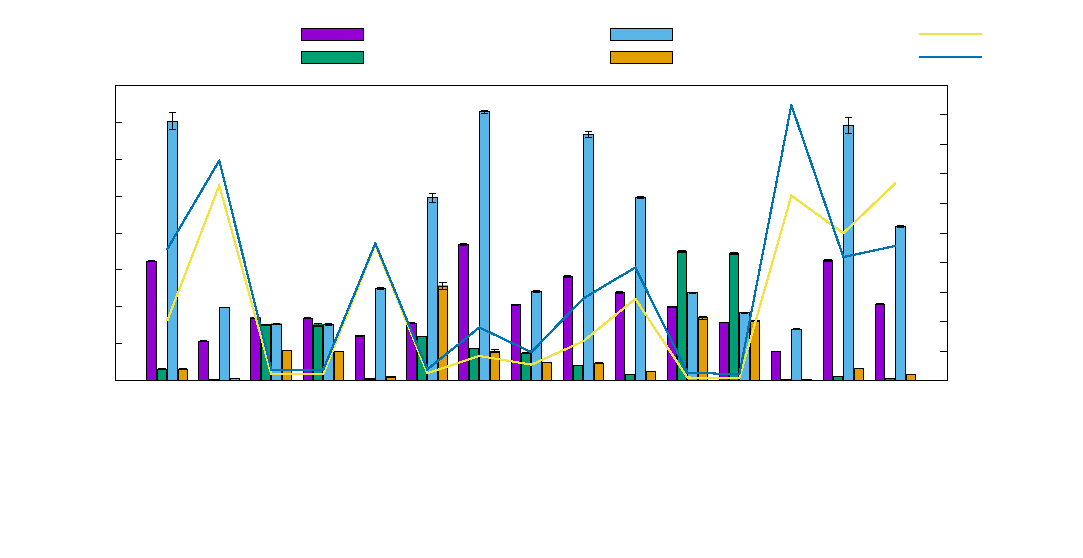
\includegraphics[width={504.00bp},height={252.00bp}]{all-hist-OnlineSetupTimesec}}%
    \gplfronttext
  \end{picture}%
\endgroup
}
% GNUPLOT: LaTeX picture with Postscript
\begingroup
  \makeatletter
  \providecommand\color[2][]{%
    \GenericError{(gnuplot) \space\space\space\@spaces}{%
      Package color not loaded in conjunction with
      terminal option `colourtext'%
    }{See the gnuplot documentation for explanation.%
    }{Either use 'blacktext' in gnuplot or load the package
      color.sty in LaTeX.}%
    \renewcommand\color[2][]{}%
  }%
  \providecommand\includegraphics[2][]{%
    \GenericError{(gnuplot) \space\space\space\@spaces}{%
      Package graphicx or graphics not loaded%
    }{See the gnuplot documentation for explanation.%
    }{The gnuplot epslatex terminal needs graphicx.sty or graphics.sty.}%
    \renewcommand\includegraphics[2][]{}%
  }%
  \providecommand\rotatebox[2]{#2}%
  \@ifundefined{ifGPcolor}{%
    \newif\ifGPcolor
    \GPcolortrue
  }{}%
  \@ifundefined{ifGPblacktext}{%
    \newif\ifGPblacktext
    \GPblacktextfalse
  }{}%
  % define a \g@addto@macro without @ in the name:
  \let\gplgaddtomacro\g@addto@macro
  % define empty templates for all commands taking text:
  \gdef\gplbacktext{}%
  \gdef\gplfronttext{}%
  \makeatother
  \ifGPblacktext
    % no textcolor at all
    \def\colorrgb#1{}%
    \def\colorgray#1{}%
  \else
    % gray or color?
    \ifGPcolor
      \def\colorrgb#1{\color[rgb]{#1}}%
      \def\colorgray#1{\color[gray]{#1}}%
      \expandafter\def\csname LTw\endcsname{\color{white}}%
      \expandafter\def\csname LTb\endcsname{\color{black}}%
      \expandafter\def\csname LTa\endcsname{\color{black}}%
      \expandafter\def\csname LT0\endcsname{\color[rgb]{1,0,0}}%
      \expandafter\def\csname LT1\endcsname{\color[rgb]{0,1,0}}%
      \expandafter\def\csname LT2\endcsname{\color[rgb]{0,0,1}}%
      \expandafter\def\csname LT3\endcsname{\color[rgb]{1,0,1}}%
      \expandafter\def\csname LT4\endcsname{\color[rgb]{0,1,1}}%
      \expandafter\def\csname LT5\endcsname{\color[rgb]{1,1,0}}%
      \expandafter\def\csname LT6\endcsname{\color[rgb]{0,0,0}}%
      \expandafter\def\csname LT7\endcsname{\color[rgb]{1,0.3,0}}%
      \expandafter\def\csname LT8\endcsname{\color[rgb]{0.5,0.5,0.5}}%
    \else
      % gray
      \def\colorrgb#1{\color{black}}%
      \def\colorgray#1{\color[gray]{#1}}%
      \expandafter\def\csname LTw\endcsname{\color{white}}%
      \expandafter\def\csname LTb\endcsname{\color{black}}%
      \expandafter\def\csname LTa\endcsname{\color{black}}%
      \expandafter\def\csname LT0\endcsname{\color{black}}%
      \expandafter\def\csname LT1\endcsname{\color{black}}%
      \expandafter\def\csname LT2\endcsname{\color{black}}%
      \expandafter\def\csname LT3\endcsname{\color{black}}%
      \expandafter\def\csname LT4\endcsname{\color{black}}%
      \expandafter\def\csname LT5\endcsname{\color{black}}%
      \expandafter\def\csname LT6\endcsname{\color{black}}%
      \expandafter\def\csname LT7\endcsname{\color{black}}%
      \expandafter\def\csname LT8\endcsname{\color{black}}%
    \fi
  \fi
    \setlength{\unitlength}{0.0500bp}%
    \ifx\gptboxheight\undefined%
      \newlength{\gptboxheight}%
      \newlength{\gptboxwidth}%
      \newsavebox{\gptboxtext}%
    \fi%
    \setlength{\fboxrule}{0.5pt}%
    \setlength{\fboxsep}{1pt}%
    \definecolor{tbcol}{rgb}{1,1,1}%
\begin{picture}(10080.00,5040.00)%
    \gplgaddtomacro\gplbacktext{%
      \csname LTb\endcsname%%
      \put(814,1100){\makebox(0,0)[r]{\strut{}$0$}}%
      \put(814,1510){\makebox(0,0)[r]{\strut{}$50$}}%
      \put(814,1920){\makebox(0,0)[r]{\strut{}$100$}}%
      \put(814,2330){\makebox(0,0)[r]{\strut{}$150$}}%
      \put(814,2740){\makebox(0,0)[r]{\strut{}$200$}}%
      \put(814,3149){\makebox(0,0)[r]{\strut{}$250$}}%
      \put(814,3559){\makebox(0,0)[r]{\strut{}$300$}}%
      \put(814,3969){\makebox(0,0)[r]{\strut{}$350$}}%
      \put(814,4379){\makebox(0,0)[r]{\strut{}$400$}}%
      \put(1416,968){\rotatebox{-45}{\makebox(0,0)[l]{\strut{}Biometric Matching}}}%
      \put(1886,968){\rotatebox{-45}{\makebox(0,0)[l]{\strut{}Biometric Matching (Fast)}}}%
      \put(2356,968){\rotatebox{-45}{\makebox(0,0)[l]{\strut{}Convex Hull}}}%
      \put(2826,968){\rotatebox{-45}{\makebox(0,0)[l]{\strut{}Count 102}}}%
      \put(3296,968){\rotatebox{-45}{\makebox(0,0)[l]{\strut{}Count 10s}}}%
      \put(3766,968){\rotatebox{-45}{\makebox(0,0)[l]{\strut{}Cryptonets (Max Pooling)}}}%
      \put(4236,968){\rotatebox{-45}{\makebox(0,0)[l]{\strut{}Database Join}}}%
      \put(4706,968){\rotatebox{-45}{\makebox(0,0)[l]{\strut{}Database Variance}}}%
      \put(5175,968){\rotatebox{-45}{\makebox(0,0)[l]{\strut{}Histogram}}}%
      \put(5645,968){\rotatebox{-45}{\makebox(0,0)[l]{\strut{}Inner Product}}}%
      \put(6115,968){\rotatebox{-45}{\makebox(0,0)[l]{\strut{}k-means}}}%
      \put(6585,968){\rotatebox{-45}{\makebox(0,0)[l]{\strut{}Longest 102}}}%
      \put(7055,968){\rotatebox{-45}{\makebox(0,0)[l]{\strut{}Max. Dist. b/w Symbols}}}%
      \put(7525,968){\rotatebox{-45}{\makebox(0,0)[l]{\strut{}Minimal Points}}}%
      \put(7995,968){\rotatebox{-45}{\makebox(0,0)[l]{\strut{}MNIST ReLU}}}%
      \put(8465,968){\rotatebox{-45}{\makebox(0,0)[l]{\strut{}Private Set Intersection}}}%
      \put(9067,1100){\makebox(0,0)[l]{\strut{}$0$}}%
      \put(9067,1568){\makebox(0,0)[l]{\strut{}$10$}}%
      \put(9067,2037){\makebox(0,0)[l]{\strut{}$20$}}%
      \put(9067,2505){\makebox(0,0)[l]{\strut{}$30$}}%
      \put(9067,2974){\makebox(0,0)[l]{\strut{}$40$}}%
      \put(9067,3442){\makebox(0,0)[l]{\strut{}$50$}}%
      \put(9067,3911){\makebox(0,0)[l]{\strut{}$60$}}%
      \put(9067,4379){\makebox(0,0)[l]{\strut{}$70$}}%
    }%
    \gplgaddtomacro\gplfronttext{%
      \csname LTb\endcsname%%
      \put(209,2739){\rotatebox{-270}{\makebox(0,0){\strut{}Online + Setup Time (sec)}}}%
      \put(9573,2739){\rotatebox{-270}{\makebox(0,0){\strut{}Improvement (number of times)}}}%
      \csname LTb\endcsname%%
      \put(2602,4867){\makebox(0,0)[r]{\strut{}GMW}}%
      \csname LTb\endcsname%%
      \put(2602,4647){\makebox(0,0)[r]{\strut{}GMW (Vectorized)}}%
      \csname LTb\endcsname%%
      \put(5569,4867){\makebox(0,0)[r]{\strut{}BMR}}%
      \csname LTb\endcsname%%
      \put(5569,4647){\makebox(0,0)[r]{\strut{}BMR (Vectorized)}}%
      \csname LTb\endcsname%%
      \put(8536,4867){\makebox(0,0)[r]{\strut{}GMW Improvement}}%
      \csname LTb\endcsname%%
      \put(8536,4647){\makebox(0,0)[r]{\strut{}BMR Improvement}}%
    }%
    \gplbacktext
    \put(0,0){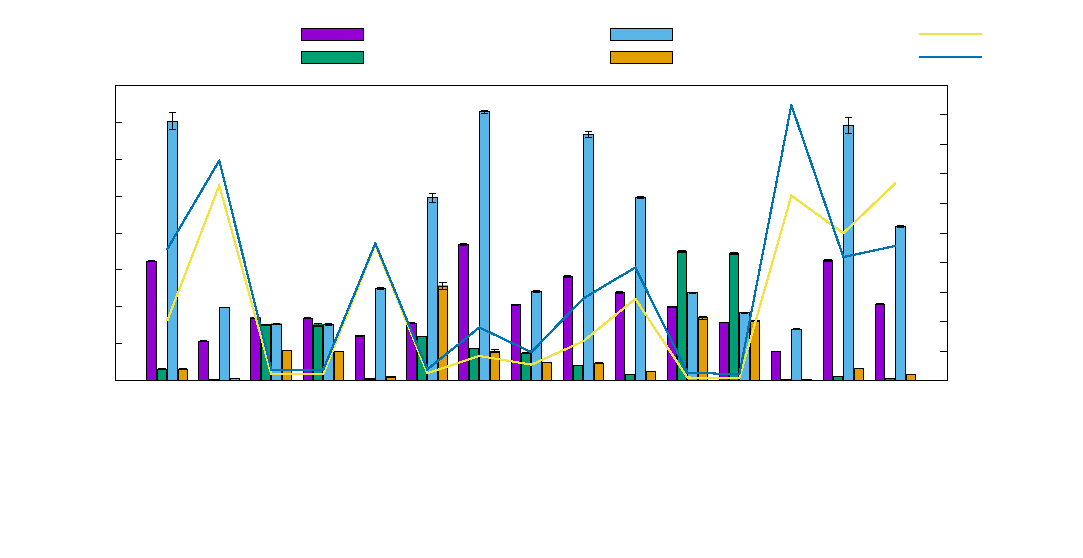
\includegraphics[width={504.00bp},height={252.00bp}]{all-hist-OnlineSetupTimesec}}%
    \gplfronttext
  \end{picture}%
\endgroup

\caption{Circuit Evaluation Time (Setup + Online) of Benchmarks}
\label{fig:graph_all_eval_time}
\end{figure*}

A detailed summery of the effects of vectorization on various benchmarks is presented in \cref{table:metrics}. We show circuit evaluation times in \cref{fig:graph_all_eval_time}. In terms of amenability to vectorization, we divide benchmarks into 3 categories: 1) {\it High:} these include convex hull, cryptonets max pooling, minimal points and private set intersection. These benchmarks are highly parallelizable and see 25x to 70x speedup in BMR, and 30x to 55x in GMW protocol. 2) {\it Medium:} these include biometric matching, DB Variance, histogram, inner product, k-means iteration and MNIST ReLU. These benchmarks have non-parallelizable phases e.g. the summing phase of inner product and biometric matching. Still, most computation is parallelizable and it results in speedup from 5x to 25x in BMR, and 2x to 25x in GMW protocol. 3) {\it Low:} these include the Database Join and the regular expression benchmarks (count 102, count 10, longest 102 and max distance between symbols). There is very little parallelizable computation in these programs, thus the speedup is lower. We see a speedup from 1.1x to 2x in BMR. In GMW, DB Join, Count 102 and Count 10s see speedup from 1.1x to 1.3x. However, longest 102 and max distance between symbols suffer a slowdown of 0.5x. The structure of these benchmarks is such that transformation to vectorized code increases multiplicative depth and, the negative effect of increased depth is more noticeable in a round-based protocol like GMW. We fix this via a simple heuristic where if the transformation increases circuit depth beyond some threshold (e.g. more than 10\% of the original circuit), we reject the transformation. Nevertheless, we show these graphs here for the sake of completeness and to highlight that vectorization is not always reduce run time. Note that in some settings it may still be desirable to vectorize e.g. in data constrained environments. As shown in \cref{fig:graph_comm_size}, vectorization results in reduced communication (fewer bits are transferred).

We present evaluation for communication size in \cref{fig:graph_comm_size_time}, circuit generation time in \cref{fig:graph_circ_gen_time}, number of gates in \cref{fig:graph_total_gates} and online time and setup time in \cref{fig:graph_online_time} and \cref{fig:graph_setup_time} respectively. \ishaq{Ana: Let me know if I should add more substance.}


\begin{figure}[htbp]
\centering
\resizebox{3.6in}{!}{\input{graphs/lan/biometric-hist-OnlineSetupTimesec}}
\caption{Biometric Matching Circuit Evaluation Time, x-axis lists database size}
\label{fig:graph_biometric_eval_time}
\end{figure}

\begin{figure}[htbp]
\centering
\resizebox{3.6in}{!}{% GNUPLOT: LaTeX picture with Postscript
\begingroup
  \makeatletter
  \providecommand\color[2][]{%
    \GenericError{(gnuplot) \space\space\space\@spaces}{%
      Package color not loaded in conjunction with
      terminal option `colourtext'%
    }{See the gnuplot documentation for explanation.%
    }{Either use 'blacktext' in gnuplot or load the package
      color.sty in LaTeX.}%
    \renewcommand\color[2][]{}%
  }%
  \providecommand\includegraphics[2][]{%
    \GenericError{(gnuplot) \space\space\space\@spaces}{%
      Package graphicx or graphics not loaded%
    }{See the gnuplot documentation for explanation.%
    }{The gnuplot epslatex terminal needs graphicx.sty or graphics.sty.}%
    \renewcommand\includegraphics[2][]{}%
  }%
  \providecommand\rotatebox[2]{#2}%
  \@ifundefined{ifGPcolor}{%
    \newif\ifGPcolor
    \GPcolortrue
  }{}%
  \@ifundefined{ifGPblacktext}{%
    \newif\ifGPblacktext
    \GPblacktextfalse
  }{}%
  % define a \g@addto@macro without @ in the name:
  \let\gplgaddtomacro\g@addto@macro
  % define empty templates for all commands taking text:
  \gdef\gplbacktext{}%
  \gdef\gplfronttext{}%
  \makeatother
  \ifGPblacktext
    % no textcolor at all
    \def\colorrgb#1{}%
    \def\colorgray#1{}%
  \else
    % gray or color?
    \ifGPcolor
      \def\colorrgb#1{\color[rgb]{#1}}%
      \def\colorgray#1{\color[gray]{#1}}%
      \expandafter\def\csname LTw\endcsname{\color{white}}%
      \expandafter\def\csname LTb\endcsname{\color{black}}%
      \expandafter\def\csname LTa\endcsname{\color{black}}%
      \expandafter\def\csname LT0\endcsname{\color[rgb]{1,0,0}}%
      \expandafter\def\csname LT1\endcsname{\color[rgb]{0,1,0}}%
      \expandafter\def\csname LT2\endcsname{\color[rgb]{0,0,1}}%
      \expandafter\def\csname LT3\endcsname{\color[rgb]{1,0,1}}%
      \expandafter\def\csname LT4\endcsname{\color[rgb]{0,1,1}}%
      \expandafter\def\csname LT5\endcsname{\color[rgb]{1,1,0}}%
      \expandafter\def\csname LT6\endcsname{\color[rgb]{0,0,0}}%
      \expandafter\def\csname LT7\endcsname{\color[rgb]{1,0.3,0}}%
      \expandafter\def\csname LT8\endcsname{\color[rgb]{0.5,0.5,0.5}}%
    \else
      % gray
      \def\colorrgb#1{\color{black}}%
      \def\colorgray#1{\color[gray]{#1}}%
      \expandafter\def\csname LTw\endcsname{\color{white}}%
      \expandafter\def\csname LTb\endcsname{\color{black}}%
      \expandafter\def\csname LTa\endcsname{\color{black}}%
      \expandafter\def\csname LT0\endcsname{\color{black}}%
      \expandafter\def\csname LT1\endcsname{\color{black}}%
      \expandafter\def\csname LT2\endcsname{\color{black}}%
      \expandafter\def\csname LT3\endcsname{\color{black}}%
      \expandafter\def\csname LT4\endcsname{\color{black}}%
      \expandafter\def\csname LT5\endcsname{\color{black}}%
      \expandafter\def\csname LT6\endcsname{\color{black}}%
      \expandafter\def\csname LT7\endcsname{\color{black}}%
      \expandafter\def\csname LT8\endcsname{\color{black}}%
    \fi
  \fi
    \setlength{\unitlength}{0.0500bp}%
    \ifx\gptboxheight\undefined%
      \newlength{\gptboxheight}%
      \newlength{\gptboxwidth}%
      \newsavebox{\gptboxtext}%
    \fi%
    \setlength{\fboxrule}{0.5pt}%
    \setlength{\fboxsep}{1pt}%
    \definecolor{tbcol}{rgb}{1,1,1}%
\begin{picture}(5760.00,4320.00)%
    \gplgaddtomacro\gplbacktext{%
      \csname LTb\endcsname%%
      \put(946,440){\makebox(0,0)[r]{\strut{}$0$}}%
      \put(946,847){\makebox(0,0)[r]{\strut{}$500$}}%
      \put(946,1253){\makebox(0,0)[r]{\strut{}$1000$}}%
      \put(946,1660){\makebox(0,0)[r]{\strut{}$1500$}}%
      \put(946,2066){\makebox(0,0)[r]{\strut{}$2000$}}%
      \put(946,2473){\makebox(0,0)[r]{\strut{}$2500$}}%
      \put(946,2879){\makebox(0,0)[r]{\strut{}$3000$}}%
      \put(946,3286){\makebox(0,0)[r]{\strut{}$3500$}}%
      \put(946,3692){\makebox(0,0)[r]{\strut{}$4000$}}%
      \put(946,4099){\makebox(0,0)[r]{\strut{}$4500$}}%
      \put(1373,308){\rotatebox{-45}{\makebox(0,0)[l]{\strut{}N: 4}}}%
      \put(1668,308){\rotatebox{-45}{\makebox(0,0)[l]{\strut{}N: 8}}}%
      \put(1962,308){\rotatebox{-45}{\makebox(0,0)[l]{\strut{}N: 16}}}%
      \put(2257,308){\rotatebox{-45}{\makebox(0,0)[l]{\strut{}N: 32}}}%
      \put(2552,308){\rotatebox{-45}{\makebox(0,0)[l]{\strut{}N: 64}}}%
      \put(2847,308){\rotatebox{-45}{\makebox(0,0)[l]{\strut{}N: 128}}}%
      \put(3141,308){\rotatebox{-45}{\makebox(0,0)[l]{\strut{}N: 256}}}%
      \put(3436,308){\rotatebox{-45}{\makebox(0,0)[l]{\strut{}N: 512}}}%
      \put(3731,308){\rotatebox{-45}{\makebox(0,0)[l]{\strut{}N: 1024}}}%
      \put(4026,308){\rotatebox{-45}{\makebox(0,0)[l]{\strut{}N: 2048}}}%
      \put(4320,308){\rotatebox{-45}{\makebox(0,0)[l]{\strut{}N: 4096}}}%
      \put(4747,440){\makebox(0,0)[l]{\strut{}$0$}}%
      \put(4747,1050){\makebox(0,0)[l]{\strut{}$2$}}%
      \put(4747,1660){\makebox(0,0)[l]{\strut{}$4$}}%
      \put(4747,2270){\makebox(0,0)[l]{\strut{}$6$}}%
      \put(4747,2879){\makebox(0,0)[l]{\strut{}$8$}}%
      \put(4747,3489){\makebox(0,0)[l]{\strut{}$10$}}%
      \put(4747,4099){\makebox(0,0)[l]{\strut{}$12$}}%
    }%
    \gplgaddtomacro\gplfronttext{%
      \csname LTb\endcsname%%
      \put(209,2269){\rotatebox{-270}{\makebox(0,0){\strut{}Communication (MiB)}}}%
      \put(5253,2269){\rotatebox{-270}{\makebox(0,0){\strut{}Improvement (number of times)}}}%
      \csname LTb\endcsname%%
      \put(3322,3926){\makebox(0,0)[r]{\strut{}GMW}}%
      \csname LTb\endcsname%%
      \put(3322,3706){\makebox(0,0)[r]{\strut{}GMW (Vectorized)}}%
      \csname LTb\endcsname%%
      \put(3322,3486){\makebox(0,0)[r]{\strut{}BMR}}%
      \csname LTb\endcsname%%
      \put(3322,3266){\makebox(0,0)[r]{\strut{}BMR (Vectorized)}}%
      \csname LTb\endcsname%%
      \put(3322,3046){\makebox(0,0)[r]{\strut{}GMW Improvement}}%
      \csname LTb\endcsname%%
      \put(3322,2826){\makebox(0,0)[r]{\strut{}BMR Improvement}}%
    }%
    \gplbacktext
    \put(0,0){\includegraphics[width={288.00bp},height={216.00bp}]{biometric-hist-CommunicationMiB}}%
    \gplfronttext
  \end{picture}%
\endgroup
}
\caption{Biometric Matching Communication Size, x-axis lists database size}
\label{fig:graph_biometic_comm_size}
\end{figure}

\begin{figure}[htbp]
\centering
\resizebox{3.6in}{!}{% GNUPLOT: LaTeX picture with Postscript
\begingroup
  \makeatletter
  \providecommand\color[2][]{%
    \GenericError{(gnuplot) \space\space\space\@spaces}{%
      Package color not loaded in conjunction with
      terminal option `colourtext'%
    }{See the gnuplot documentation for explanation.%
    }{Either use 'blacktext' in gnuplot or load the package
      color.sty in LaTeX.}%
    \renewcommand\color[2][]{}%
  }%
  \providecommand\includegraphics[2][]{%
    \GenericError{(gnuplot) \space\space\space\@spaces}{%
      Package graphicx or graphics not loaded%
    }{See the gnuplot documentation for explanation.%
    }{The gnuplot epslatex terminal needs graphicx.sty or graphics.sty.}%
    \renewcommand\includegraphics[2][]{}%
  }%
  \providecommand\rotatebox[2]{#2}%
  \@ifundefined{ifGPcolor}{%
    \newif\ifGPcolor
    \GPcolortrue
  }{}%
  \@ifundefined{ifGPblacktext}{%
    \newif\ifGPblacktext
    \GPblacktextfalse
  }{}%
  % define a \g@addto@macro without @ in the name:
  \let\gplgaddtomacro\g@addto@macro
  % define empty templates for all commands taking text:
  \gdef\gplbacktext{}%
  \gdef\gplfronttext{}%
  \makeatother
  \ifGPblacktext
    % no textcolor at all
    \def\colorrgb#1{}%
    \def\colorgray#1{}%
  \else
    % gray or color?
    \ifGPcolor
      \def\colorrgb#1{\color[rgb]{#1}}%
      \def\colorgray#1{\color[gray]{#1}}%
      \expandafter\def\csname LTw\endcsname{\color{white}}%
      \expandafter\def\csname LTb\endcsname{\color{black}}%
      \expandafter\def\csname LTa\endcsname{\color{black}}%
      \expandafter\def\csname LT0\endcsname{\color[rgb]{1,0,0}}%
      \expandafter\def\csname LT1\endcsname{\color[rgb]{0,1,0}}%
      \expandafter\def\csname LT2\endcsname{\color[rgb]{0,0,1}}%
      \expandafter\def\csname LT3\endcsname{\color[rgb]{1,0,1}}%
      \expandafter\def\csname LT4\endcsname{\color[rgb]{0,1,1}}%
      \expandafter\def\csname LT5\endcsname{\color[rgb]{1,1,0}}%
      \expandafter\def\csname LT6\endcsname{\color[rgb]{0,0,0}}%
      \expandafter\def\csname LT7\endcsname{\color[rgb]{1,0.3,0}}%
      \expandafter\def\csname LT8\endcsname{\color[rgb]{0.5,0.5,0.5}}%
    \else
      % gray
      \def\colorrgb#1{\color{black}}%
      \def\colorgray#1{\color[gray]{#1}}%
      \expandafter\def\csname LTw\endcsname{\color{white}}%
      \expandafter\def\csname LTb\endcsname{\color{black}}%
      \expandafter\def\csname LTa\endcsname{\color{black}}%
      \expandafter\def\csname LT0\endcsname{\color{black}}%
      \expandafter\def\csname LT1\endcsname{\color{black}}%
      \expandafter\def\csname LT2\endcsname{\color{black}}%
      \expandafter\def\csname LT3\endcsname{\color{black}}%
      \expandafter\def\csname LT4\endcsname{\color{black}}%
      \expandafter\def\csname LT5\endcsname{\color{black}}%
      \expandafter\def\csname LT6\endcsname{\color{black}}%
      \expandafter\def\csname LT7\endcsname{\color{black}}%
      \expandafter\def\csname LT8\endcsname{\color{black}}%
    \fi
  \fi
    \setlength{\unitlength}{0.0500bp}%
    \ifx\gptboxheight\undefined%
      \newlength{\gptboxheight}%
      \newlength{\gptboxwidth}%
      \newsavebox{\gptboxtext}%
    \fi%
    \setlength{\fboxrule}{0.5pt}%
    \setlength{\fboxsep}{1pt}%
    \definecolor{tbcol}{rgb}{1,1,1}%
\begin{picture}(5760.00,4320.00)%
    \gplgaddtomacro\gplbacktext{%
      \csname LTb\endcsname%%
      \put(814,440){\makebox(0,0)[r]{\strut{}$0$}}%
      \put(814,963){\makebox(0,0)[r]{\strut{}$20$}}%
      \put(814,1485){\makebox(0,0)[r]{\strut{}$40$}}%
      \put(814,2008){\makebox(0,0)[r]{\strut{}$60$}}%
      \put(814,2531){\makebox(0,0)[r]{\strut{}$80$}}%
      \put(814,3054){\makebox(0,0)[r]{\strut{}$100$}}%
      \put(814,3576){\makebox(0,0)[r]{\strut{}$120$}}%
      \put(814,4099){\makebox(0,0)[r]{\strut{}$140$}}%
      \put(1252,308){\rotatebox{-45}{\makebox(0,0)[l]{\strut{}N: 4}}}%
      \put(1558,308){\rotatebox{-45}{\makebox(0,0)[l]{\strut{}N: 8}}}%
      \put(1863,308){\rotatebox{-45}{\makebox(0,0)[l]{\strut{}N: 16}}}%
      \put(2169,308){\rotatebox{-45}{\makebox(0,0)[l]{\strut{}N: 32}}}%
      \put(2475,308){\rotatebox{-45}{\makebox(0,0)[l]{\strut{}N: 64}}}%
      \put(2781,308){\rotatebox{-45}{\makebox(0,0)[l]{\strut{}N: 128}}}%
      \put(3086,308){\rotatebox{-45}{\makebox(0,0)[l]{\strut{}N: 256}}}%
      \put(3392,308){\rotatebox{-45}{\makebox(0,0)[l]{\strut{}N: 512}}}%
      \put(3698,308){\rotatebox{-45}{\makebox(0,0)[l]{\strut{}N: 1024}}}%
      \put(4004,308){\rotatebox{-45}{\makebox(0,0)[l]{\strut{}N: 2048}}}%
      \put(4309,308){\rotatebox{-45}{\makebox(0,0)[l]{\strut{}N: 4096}}}%
      \put(4747,440){\makebox(0,0)[l]{\strut{}$0$}}%
      \put(4747,806){\makebox(0,0)[l]{\strut{}$5$}}%
      \put(4747,1172){\makebox(0,0)[l]{\strut{}$10$}}%
      \put(4747,1538){\makebox(0,0)[l]{\strut{}$15$}}%
      \put(4747,1904){\makebox(0,0)[l]{\strut{}$20$}}%
      \put(4747,2270){\makebox(0,0)[l]{\strut{}$25$}}%
      \put(4747,2635){\makebox(0,0)[l]{\strut{}$30$}}%
      \put(4747,3001){\makebox(0,0)[l]{\strut{}$35$}}%
      \put(4747,3367){\makebox(0,0)[l]{\strut{}$40$}}%
      \put(4747,3733){\makebox(0,0)[l]{\strut{}$45$}}%
      \put(4747,4099){\makebox(0,0)[l]{\strut{}$50$}}%
    }%
    \gplgaddtomacro\gplfronttext{%
      \csname LTb\endcsname%%
      \put(209,2269){\rotatebox{-270}{\makebox(0,0){\strut{}Circuit Generation Time (sec)}}}%
      \put(5253,2269){\rotatebox{-270}{\makebox(0,0){\strut{}Improvement (number of times)}}}%
      \csname LTb\endcsname%%
      \put(3190,3926){\makebox(0,0)[r]{\strut{}GMW}}%
      \csname LTb\endcsname%%
      \put(3190,3706){\makebox(0,0)[r]{\strut{}GMW (Vectorized)}}%
      \csname LTb\endcsname%%
      \put(3190,3486){\makebox(0,0)[r]{\strut{}BMR}}%
      \csname LTb\endcsname%%
      \put(3190,3266){\makebox(0,0)[r]{\strut{}BMR (Vectorized)}}%
      \csname LTb\endcsname%%
      \put(3190,3046){\makebox(0,0)[r]{\strut{}GMW Improvement}}%
      \csname LTb\endcsname%%
      \put(3190,2826){\makebox(0,0)[r]{\strut{}BMR Improvement}}%
    }%
    \gplbacktext
    \put(0,0){\includegraphics[width={288.00bp},height={216.00bp}]{biometric-hist-CircuitGenerationTimesec}}%
    \gplfronttext
  \end{picture}%
\endgroup
}
\caption{Biometric Matching Circuit Generation Time, x-axis lists database size}
\label{fig:graph_biometic_circ_gen_time}
\end{figure}

Next, we look closely at circuit evaluation \cref{fig:graph_biometric_eval_time}, communication size \cref{fig:graph_biometic_comm_size} and circuit generation time \cref{fig:graph_biometic_circ_gen_time} for biometric matching benchmark. For input size beyond {\tt N=128} the memory usage exceeds available memory and prevents circuit generation. Consequently, non-vectorized bars are missing beyond this threshold. Notice that vectorization improves all metrics. A database of size {\tt N=128} is smaller than any real world usecase, therefore lets use it as baseline for improvement. Comparing performance improvement between BMR and GMW, we see more speedup for BMR (23x vs 10x), GMW gets more communication size reduction (10x vs 2.5x) and circuit generation sees a speedup of 35x and 45x for BMR and GMW respectively. 



\begin{figure}[htbp]
\centering
\resizebox{3.6in}{!}{% GNUPLOT: LaTeX picture with Postscript
\begingroup
  \makeatletter
  \providecommand\color[2][]{%
    \GenericError{(gnuplot) \space\space\space\@spaces}{%
      Package color not loaded in conjunction with
      terminal option `colourtext'%
    }{See the gnuplot documentation for explanation.%
    }{Either use 'blacktext' in gnuplot or load the package
      color.sty in LaTeX.}%
    \renewcommand\color[2][]{}%
  }%
  \providecommand\includegraphics[2][]{%
    \GenericError{(gnuplot) \space\space\space\@spaces}{%
      Package graphicx or graphics not loaded%
    }{See the gnuplot documentation for explanation.%
    }{The gnuplot epslatex terminal needs graphicx.sty or graphics.sty.}%
    \renewcommand\includegraphics[2][]{}%
  }%
  \providecommand\rotatebox[2]{#2}%
  \@ifundefined{ifGPcolor}{%
    \newif\ifGPcolor
    \GPcolortrue
  }{}%
  \@ifundefined{ifGPblacktext}{%
    \newif\ifGPblacktext
    \GPblacktextfalse
  }{}%
  % define a \g@addto@macro without @ in the name:
  \let\gplgaddtomacro\g@addto@macro
  % define empty templates for all commands taking text:
  \gdef\gplbacktext{}%
  \gdef\gplfronttext{}%
  \makeatother
  \ifGPblacktext
    % no textcolor at all
    \def\colorrgb#1{}%
    \def\colorgray#1{}%
  \else
    % gray or color?
    \ifGPcolor
      \def\colorrgb#1{\color[rgb]{#1}}%
      \def\colorgray#1{\color[gray]{#1}}%
      \expandafter\def\csname LTw\endcsname{\color{white}}%
      \expandafter\def\csname LTb\endcsname{\color{black}}%
      \expandafter\def\csname LTa\endcsname{\color{black}}%
      \expandafter\def\csname LT0\endcsname{\color[rgb]{1,0,0}}%
      \expandafter\def\csname LT1\endcsname{\color[rgb]{0,1,0}}%
      \expandafter\def\csname LT2\endcsname{\color[rgb]{0,0,1}}%
      \expandafter\def\csname LT3\endcsname{\color[rgb]{1,0,1}}%
      \expandafter\def\csname LT4\endcsname{\color[rgb]{0,1,1}}%
      \expandafter\def\csname LT5\endcsname{\color[rgb]{1,1,0}}%
      \expandafter\def\csname LT6\endcsname{\color[rgb]{0,0,0}}%
      \expandafter\def\csname LT7\endcsname{\color[rgb]{1,0.3,0}}%
      \expandafter\def\csname LT8\endcsname{\color[rgb]{0.5,0.5,0.5}}%
    \else
      % gray
      \def\colorrgb#1{\color{black}}%
      \def\colorgray#1{\color[gray]{#1}}%
      \expandafter\def\csname LTw\endcsname{\color{white}}%
      \expandafter\def\csname LTb\endcsname{\color{black}}%
      \expandafter\def\csname LTa\endcsname{\color{black}}%
      \expandafter\def\csname LT0\endcsname{\color{black}}%
      \expandafter\def\csname LT1\endcsname{\color{black}}%
      \expandafter\def\csname LT2\endcsname{\color{black}}%
      \expandafter\def\csname LT3\endcsname{\color{black}}%
      \expandafter\def\csname LT4\endcsname{\color{black}}%
      \expandafter\def\csname LT5\endcsname{\color{black}}%
      \expandafter\def\csname LT6\endcsname{\color{black}}%
      \expandafter\def\csname LT7\endcsname{\color{black}}%
      \expandafter\def\csname LT8\endcsname{\color{black}}%
    \fi
  \fi
    \setlength{\unitlength}{0.0500bp}%
    \ifx\gptboxheight\undefined%
      \newlength{\gptboxheight}%
      \newlength{\gptboxwidth}%
      \newsavebox{\gptboxtext}%
    \fi%
    \setlength{\fboxrule}{0.5pt}%
    \setlength{\fboxsep}{1pt}%
    \definecolor{tbcol}{rgb}{1,1,1}%
\begin{picture}(5760.00,4320.00)%
    \gplgaddtomacro\gplbacktext{%
      \csname LTb\endcsname%%
      \put(946,660){\makebox(0,0)[r]{\strut{}$0$}}%
      \csname LTb\endcsname%%
      \put(946,1151){\makebox(0,0)[r]{\strut{}$500$}}%
      \csname LTb\endcsname%%
      \put(946,1643){\makebox(0,0)[r]{\strut{}$1000$}}%
      \csname LTb\endcsname%%
      \put(946,2134){\makebox(0,0)[r]{\strut{}$1500$}}%
      \csname LTb\endcsname%%
      \put(946,2625){\makebox(0,0)[r]{\strut{}$2000$}}%
      \csname LTb\endcsname%%
      \put(946,3116){\makebox(0,0)[r]{\strut{}$2500$}}%
      \csname LTb\endcsname%%
      \put(946,3608){\makebox(0,0)[r]{\strut{}$3000$}}%
      \csname LTb\endcsname%%
      \put(946,4099){\makebox(0,0)[r]{\strut{}$3500$}}%
      \csname LTb\endcsname%%
      \put(2149,528){\rotatebox{-25}{\makebox(0,0)[l]{\strut{}Biometric Matching}}}%
      \csname LTb\endcsname%%
      \put(3221,528){\rotatebox{-25}{\makebox(0,0)[l]{\strut{}Inner Product}}}%
      \csname LTb\endcsname%%
      \put(4292,528){\rotatebox{-25}{\makebox(0,0)[l]{\strut{}Longest 102}}}%
    }%
    \gplgaddtomacro\gplfronttext{%
      \csname LTb\endcsname%%
      \put(209,2379){\rotatebox{-270}{\makebox(0,0){\strut{}Online + Setup Time (sec)}}}%
      \csname LTb\endcsname%%
      \put(2134,3926){\makebox(0,0)[r]{\strut{}GMW LAN}}%
      \csname LTb\endcsname%%
      \put(2134,3706){\makebox(0,0)[r]{\strut{}GMW WAN}}%
      \csname LTb\endcsname%%
      \put(2134,3486){\makebox(0,0)[r]{\strut{}BMR LAN}}%
      \csname LTb\endcsname%%
      \put(2134,3266){\makebox(0,0)[r]{\strut{}BMR WAN}}%
    }%
    \gplbacktext
    \put(0,0){\includegraphics[width={288.00bp},height={216.00bp}]{comparison-hist-OnlineSetupTimesec}}%
    \gplfronttext
  \end{picture}%
\endgroup
}
\caption{LAN vs. WAN: Circuit Evaluation Time Comparison}
\label{fig:graph_comparison_eval_time}
\end{figure}

Since our vectorization framework is network agnostic, it produces the same circuit for both LAN and WAN. This means that the number of gates and communication size remain the same. Moreover, time for circuit generation, which is a local operation, also remains unchanged. Setup and Online times, however, increase due to lower bandwidth and higher latency of the WAN. Indeed, this is what we observe in \cref{fig:graph_comparison_eval_time}.

\begin{figure*}[htbp]
\centering
% GNUPLOT: LaTeX picture with Postscript
\begingroup
  \makeatletter
  \providecommand\color[2][]{%
    \GenericError{(gnuplot) \space\space\space\@spaces}{%
      Package color not loaded in conjunction with
      terminal option `colourtext'%
    }{See the gnuplot documentation for explanation.%
    }{Either use 'blacktext' in gnuplot or load the package
      color.sty in LaTeX.}%
    \renewcommand\color[2][]{}%
  }%
  \providecommand\includegraphics[2][]{%
    \GenericError{(gnuplot) \space\space\space\@spaces}{%
      Package graphicx or graphics not loaded%
    }{See the gnuplot documentation for explanation.%
    }{The gnuplot epslatex terminal needs graphicx.sty or graphics.sty.}%
    \renewcommand\includegraphics[2][]{}%
  }%
  \providecommand\rotatebox[2]{#2}%
  \@ifundefined{ifGPcolor}{%
    \newif\ifGPcolor
    \GPcolortrue
  }{}%
  \@ifundefined{ifGPblacktext}{%
    \newif\ifGPblacktext
    \GPblacktextfalse
  }{}%
  % define a \g@addto@macro without @ in the name:
  \let\gplgaddtomacro\g@addto@macro
  % define empty templates for all commands taking text:
  \gdef\gplbacktext{}%
  \gdef\gplfronttext{}%
  \makeatother
  \ifGPblacktext
    % no textcolor at all
    \def\colorrgb#1{}%
    \def\colorgray#1{}%
  \else
    % gray or color?
    \ifGPcolor
      \def\colorrgb#1{\color[rgb]{#1}}%
      \def\colorgray#1{\color[gray]{#1}}%
      \expandafter\def\csname LTw\endcsname{\color{white}}%
      \expandafter\def\csname LTb\endcsname{\color{black}}%
      \expandafter\def\csname LTa\endcsname{\color{black}}%
      \expandafter\def\csname LT0\endcsname{\color[rgb]{1,0,0}}%
      \expandafter\def\csname LT1\endcsname{\color[rgb]{0,1,0}}%
      \expandafter\def\csname LT2\endcsname{\color[rgb]{0,0,1}}%
      \expandafter\def\csname LT3\endcsname{\color[rgb]{1,0,1}}%
      \expandafter\def\csname LT4\endcsname{\color[rgb]{0,1,1}}%
      \expandafter\def\csname LT5\endcsname{\color[rgb]{1,1,0}}%
      \expandafter\def\csname LT6\endcsname{\color[rgb]{0,0,0}}%
      \expandafter\def\csname LT7\endcsname{\color[rgb]{1,0.3,0}}%
      \expandafter\def\csname LT8\endcsname{\color[rgb]{0.5,0.5,0.5}}%
    \else
      % gray
      \def\colorrgb#1{\color{black}}%
      \def\colorgray#1{\color[gray]{#1}}%
      \expandafter\def\csname LTw\endcsname{\color{white}}%
      \expandafter\def\csname LTb\endcsname{\color{black}}%
      \expandafter\def\csname LTa\endcsname{\color{black}}%
      \expandafter\def\csname LT0\endcsname{\color{black}}%
      \expandafter\def\csname LT1\endcsname{\color{black}}%
      \expandafter\def\csname LT2\endcsname{\color{black}}%
      \expandafter\def\csname LT3\endcsname{\color{black}}%
      \expandafter\def\csname LT4\endcsname{\color{black}}%
      \expandafter\def\csname LT5\endcsname{\color{black}}%
      \expandafter\def\csname LT6\endcsname{\color{black}}%
      \expandafter\def\csname LT7\endcsname{\color{black}}%
      \expandafter\def\csname LT8\endcsname{\color{black}}%
    \fi
  \fi
    \setlength{\unitlength}{0.0500bp}%
    \ifx\gptboxheight\undefined%
      \newlength{\gptboxheight}%
      \newlength{\gptboxwidth}%
      \newsavebox{\gptboxtext}%
    \fi%
    \setlength{\fboxrule}{0.5pt}%
    \setlength{\fboxsep}{1pt}%
    \definecolor{tbcol}{rgb}{1,1,1}%
\begin{picture}(10080.00,5040.00)%
    \gplgaddtomacro\gplbacktext{%
      \csname LTb\endcsname%%
      \put(814,1540){\makebox(0,0)[r]{\strut{}$0$}}%
      \put(814,1855){\makebox(0,0)[r]{\strut{}$50$}}%
      \put(814,2171){\makebox(0,0)[r]{\strut{}$100$}}%
      \put(814,2486){\makebox(0,0)[r]{\strut{}$150$}}%
      \put(814,2802){\makebox(0,0)[r]{\strut{}$200$}}%
      \put(814,3117){\makebox(0,0)[r]{\strut{}$250$}}%
      \put(814,3433){\makebox(0,0)[r]{\strut{}$300$}}%
      \put(814,3748){\makebox(0,0)[r]{\strut{}$350$}}%
      \put(814,4064){\makebox(0,0)[r]{\strut{}$400$}}%
      \put(814,4379){\makebox(0,0)[r]{\strut{}$450$}}%
      \put(1416,1408){\rotatebox{-45}{\makebox(0,0)[l]{\strut{}Biometric Matching}}}%
      \put(1886,1408){\rotatebox{-45}{\makebox(0,0)[l]{\strut{}Biometric Matching (Fast)}}}%
      \put(2356,1408){\rotatebox{-45}{\makebox(0,0)[l]{\strut{}Convex Hull}}}%
      \put(2826,1408){\rotatebox{-45}{\makebox(0,0)[l]{\strut{}Count 102}}}%
      \put(3296,1408){\rotatebox{-45}{\makebox(0,0)[l]{\strut{}Count 10s}}}%
      \put(3766,1408){\rotatebox{-45}{\makebox(0,0)[l]{\strut{}Cryptonets (Max Pooling)}}}%
      \put(4236,1408){\rotatebox{-45}{\makebox(0,0)[l]{\strut{}Database Join}}}%
      \put(4706,1408){\rotatebox{-45}{\makebox(0,0)[l]{\strut{}Database Variance}}}%
      \put(5175,1408){\rotatebox{-45}{\makebox(0,0)[l]{\strut{}Histogram}}}%
      \put(5645,1408){\rotatebox{-45}{\makebox(0,0)[l]{\strut{}Inner Product}}}%
      \put(6115,1408){\rotatebox{-45}{\makebox(0,0)[l]{\strut{}k-means}}}%
      \put(6585,1408){\rotatebox{-45}{\makebox(0,0)[l]{\strut{}Longest 102}}}%
      \put(7055,1408){\rotatebox{-45}{\makebox(0,0)[l]{\strut{}Max. Dist. b/w Symbols}}}%
      \put(7525,1408){\rotatebox{-45}{\makebox(0,0)[l]{\strut{}Minimal Points}}}%
      \put(7995,1408){\rotatebox{-45}{\makebox(0,0)[l]{\strut{}MNIST ReLU}}}%
      \put(8465,1408){\rotatebox{-45}{\makebox(0,0)[l]{\strut{}Private Set Intersection}}}%
      \put(9067,1540){\makebox(0,0)[l]{\strut{}$0$}}%
      \put(9067,1946){\makebox(0,0)[l]{\strut{}$2$}}%
      \put(9067,2351){\makebox(0,0)[l]{\strut{}$4$}}%
      \put(9067,2757){\makebox(0,0)[l]{\strut{}$6$}}%
      \put(9067,3162){\makebox(0,0)[l]{\strut{}$8$}}%
      \put(9067,3568){\makebox(0,0)[l]{\strut{}$10$}}%
      \put(9067,3973){\makebox(0,0)[l]{\strut{}$12$}}%
      \put(9067,4379){\makebox(0,0)[l]{\strut{}$14$}}%
    }%
    \gplgaddtomacro\gplfronttext{%
      \csname LTb\endcsname%%
      \put(209,2959){\rotatebox{-270}{\makebox(0,0){\strut{}Communication (MiB)}}}%
      \put(9573,2959){\rotatebox{-270}{\makebox(0,0){\strut{}Improvement (number of times)}}}%
      \csname LTb\endcsname%%
      \put(2602,4867){\makebox(0,0)[r]{\strut{}GMW}}%
      \csname LTb\endcsname%%
      \put(2602,4647){\makebox(0,0)[r]{\strut{}GMW (Vectorized)}}%
      \csname LTb\endcsname%%
      \put(5569,4867){\makebox(0,0)[r]{\strut{}BMR}}%
      \csname LTb\endcsname%%
      \put(5569,4647){\makebox(0,0)[r]{\strut{}BMR (Vectorized)}}%
      \csname LTb\endcsname%%
      \put(8536,4867){\makebox(0,0)[r]{\strut{}GMW Improvement}}%
      \csname LTb\endcsname%%
      \put(8536,4647){\makebox(0,0)[r]{\strut{}BMR Improvement}}%
    }%
    \gplbacktext
    \put(0,0){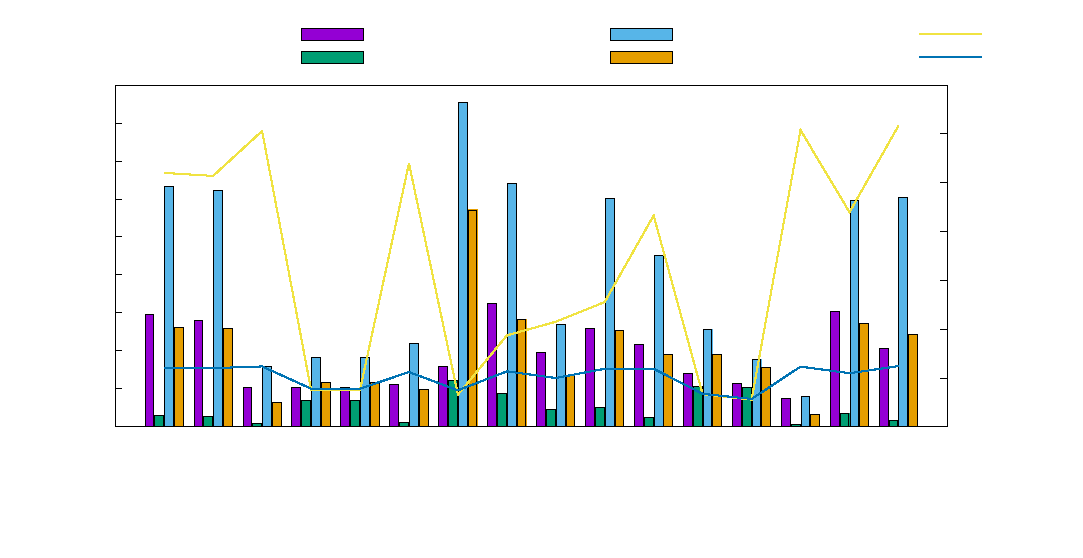
\includegraphics[width={504.00bp},height={252.00bp}]{all-hist-CommunicationMiB}}%
    \gplfronttext
  \end{picture}%
\endgroup

\caption{Communication Size of Benchmarks}
\label{fig:graph_comm_size}
\end{figure*}


\begin{figure*}[htbp]
\centering
% GNUPLOT: LaTeX picture with Postscript
\begingroup
  \makeatletter
  \providecommand\color[2][]{%
    \GenericError{(gnuplot) \space\space\space\@spaces}{%
      Package color not loaded in conjunction with
      terminal option `colourtext'%
    }{See the gnuplot documentation for explanation.%
    }{Either use 'blacktext' in gnuplot or load the package
      color.sty in LaTeX.}%
    \renewcommand\color[2][]{}%
  }%
  \providecommand\includegraphics[2][]{%
    \GenericError{(gnuplot) \space\space\space\@spaces}{%
      Package graphicx or graphics not loaded%
    }{See the gnuplot documentation for explanation.%
    }{The gnuplot epslatex terminal needs graphicx.sty or graphics.sty.}%
    \renewcommand\includegraphics[2][]{}%
  }%
  \providecommand\rotatebox[2]{#2}%
  \@ifundefined{ifGPcolor}{%
    \newif\ifGPcolor
    \GPcolortrue
  }{}%
  \@ifundefined{ifGPblacktext}{%
    \newif\ifGPblacktext
    \GPblacktextfalse
  }{}%
  % define a \g@addto@macro without @ in the name:
  \let\gplgaddtomacro\g@addto@macro
  % define empty templates for all commands taking text:
  \gdef\gplbacktext{}%
  \gdef\gplfronttext{}%
  \makeatother
  \ifGPblacktext
    % no textcolor at all
    \def\colorrgb#1{}%
    \def\colorgray#1{}%
  \else
    % gray or color?
    \ifGPcolor
      \def\colorrgb#1{\color[rgb]{#1}}%
      \def\colorgray#1{\color[gray]{#1}}%
      \expandafter\def\csname LTw\endcsname{\color{white}}%
      \expandafter\def\csname LTb\endcsname{\color{black}}%
      \expandafter\def\csname LTa\endcsname{\color{black}}%
      \expandafter\def\csname LT0\endcsname{\color[rgb]{1,0,0}}%
      \expandafter\def\csname LT1\endcsname{\color[rgb]{0,1,0}}%
      \expandafter\def\csname LT2\endcsname{\color[rgb]{0,0,1}}%
      \expandafter\def\csname LT3\endcsname{\color[rgb]{1,0,1}}%
      \expandafter\def\csname LT4\endcsname{\color[rgb]{0,1,1}}%
      \expandafter\def\csname LT5\endcsname{\color[rgb]{1,1,0}}%
      \expandafter\def\csname LT6\endcsname{\color[rgb]{0,0,0}}%
      \expandafter\def\csname LT7\endcsname{\color[rgb]{1,0.3,0}}%
      \expandafter\def\csname LT8\endcsname{\color[rgb]{0.5,0.5,0.5}}%
    \else
      % gray
      \def\colorrgb#1{\color{black}}%
      \def\colorgray#1{\color[gray]{#1}}%
      \expandafter\def\csname LTw\endcsname{\color{white}}%
      \expandafter\def\csname LTb\endcsname{\color{black}}%
      \expandafter\def\csname LTa\endcsname{\color{black}}%
      \expandafter\def\csname LT0\endcsname{\color{black}}%
      \expandafter\def\csname LT1\endcsname{\color{black}}%
      \expandafter\def\csname LT2\endcsname{\color{black}}%
      \expandafter\def\csname LT3\endcsname{\color{black}}%
      \expandafter\def\csname LT4\endcsname{\color{black}}%
      \expandafter\def\csname LT5\endcsname{\color{black}}%
      \expandafter\def\csname LT6\endcsname{\color{black}}%
      \expandafter\def\csname LT7\endcsname{\color{black}}%
      \expandafter\def\csname LT8\endcsname{\color{black}}%
    \fi
  \fi
    \setlength{\unitlength}{0.0500bp}%
    \ifx\gptboxheight\undefined%
      \newlength{\gptboxheight}%
      \newlength{\gptboxwidth}%
      \newsavebox{\gptboxtext}%
    \fi%
    \setlength{\fboxrule}{0.5pt}%
    \setlength{\fboxsep}{1pt}%
    \definecolor{tbcol}{rgb}{1,1,1}%
\begin{picture}(10080.00,5040.00)%
    \gplgaddtomacro\gplbacktext{%
      \csname LTb\endcsname%%
      \put(814,1540){\makebox(0,0)[r]{\strut{}$0$}}%
      \put(814,1895){\makebox(0,0)[r]{\strut{}$20$}}%
      \put(814,2250){\makebox(0,0)[r]{\strut{}$40$}}%
      \put(814,2605){\makebox(0,0)[r]{\strut{}$60$}}%
      \put(814,2960){\makebox(0,0)[r]{\strut{}$80$}}%
      \put(814,3314){\makebox(0,0)[r]{\strut{}$100$}}%
      \put(814,3669){\makebox(0,0)[r]{\strut{}$120$}}%
      \put(814,4024){\makebox(0,0)[r]{\strut{}$140$}}%
      \put(814,4379){\makebox(0,0)[r]{\strut{}$160$}}%
      \put(1437,1408){\rotatebox{-45}{\makebox(0,0)[l]{\strut{}Biometric Matching}}}%
      \put(1928,1408){\rotatebox{-45}{\makebox(0,0)[l]{\strut{}Convex Hull}}}%
      \put(2419,1408){\rotatebox{-45}{\makebox(0,0)[l]{\strut{}Count 102}}}%
      \put(2910,1408){\rotatebox{-45}{\makebox(0,0)[l]{\strut{}Count 10s}}}%
      \put(3401,1408){\rotatebox{-45}{\makebox(0,0)[l]{\strut{}Cryptonets (Max Pooling)}}}%
      \put(3892,1408){\rotatebox{-45}{\makebox(0,0)[l]{\strut{}Database Join}}}%
      \put(4383,1408){\rotatebox{-45}{\makebox(0,0)[l]{\strut{}Database Variance}}}%
      \put(4875,1408){\rotatebox{-45}{\makebox(0,0)[l]{\strut{}Histogram}}}%
      \put(5366,1408){\rotatebox{-45}{\makebox(0,0)[l]{\strut{}Inner Product}}}%
      \put(5857,1408){\rotatebox{-45}{\makebox(0,0)[l]{\strut{}k-means}}}%
      \put(6348,1408){\rotatebox{-45}{\makebox(0,0)[l]{\strut{}Longest 102}}}%
      \put(6839,1408){\rotatebox{-45}{\makebox(0,0)[l]{\strut{}Max. Dist. b/w Symbols}}}%
      \put(7330,1408){\rotatebox{-45}{\makebox(0,0)[l]{\strut{}Minimal Points}}}%
      \put(7821,1408){\rotatebox{-45}{\makebox(0,0)[l]{\strut{}MNIST ReLU}}}%
      \put(8312,1408){\rotatebox{-45}{\makebox(0,0)[l]{\strut{}Private Set Intersection}}}%
      \put(8935,1540){\makebox(0,0)[l]{\strut{}$0$}}%
      \put(8935,1824){\makebox(0,0)[l]{\strut{}$20$}}%
      \put(8935,2108){\makebox(0,0)[l]{\strut{}$40$}}%
      \put(8935,2392){\makebox(0,0)[l]{\strut{}$60$}}%
      \put(8935,2676){\makebox(0,0)[l]{\strut{}$80$}}%
      \put(8935,2960){\makebox(0,0)[l]{\strut{}$100$}}%
      \put(8935,3243){\makebox(0,0)[l]{\strut{}$120$}}%
      \put(8935,3527){\makebox(0,0)[l]{\strut{}$140$}}%
      \put(8935,3811){\makebox(0,0)[l]{\strut{}$160$}}%
      \put(8935,4095){\makebox(0,0)[l]{\strut{}$180$}}%
      \put(8935,4379){\makebox(0,0)[l]{\strut{}$200$}}%
    }%
    \gplgaddtomacro\gplfronttext{%
      \csname LTb\endcsname%%
      \put(209,2959){\rotatebox{-270}{\makebox(0,0){\strut{}Circuit Generation Time (sec)}}}%
      \put(9573,2959){\rotatebox{-270}{\makebox(0,0){\strut{}Improvement (number of times)}}}%
      \csname LTb\endcsname%%
      \put(2536,4867){\makebox(0,0)[r]{\strut{}GMW}}%
      \csname LTb\endcsname%%
      \put(2536,4647){\makebox(0,0)[r]{\strut{}GMW (Vectorized)}}%
      \csname LTb\endcsname%%
      \put(5503,4867){\makebox(0,0)[r]{\strut{}BMR}}%
      \csname LTb\endcsname%%
      \put(5503,4647){\makebox(0,0)[r]{\strut{}BMR (Vectorized)}}%
      \csname LTb\endcsname%%
      \put(8470,4867){\makebox(0,0)[r]{\strut{}GMW Improvement}}%
      \csname LTb\endcsname%%
      \put(8470,4647){\makebox(0,0)[r]{\strut{}BMR Improvement}}%
    }%
    \gplbacktext
    \put(0,0){\includegraphics[width={504.00bp},height={252.00bp}]{all-hist-CircuitGenerationTimesec}}%
    \gplfronttext
  \end{picture}%
\endgroup

\caption{Circuit Generation Time of Benchmarks}
\label{fig:graph_circ_gen_time}
\end{figure*}

\begin{figure*}[htbp]
\centering
% GNUPLOT: LaTeX picture with Postscript
\begingroup
  \makeatletter
  \providecommand\color[2][]{%
    \GenericError{(gnuplot) \space\space\space\@spaces}{%
      Package color not loaded in conjunction with
      terminal option `colourtext'%
    }{See the gnuplot documentation for explanation.%
    }{Either use 'blacktext' in gnuplot or load the package
      color.sty in LaTeX.}%
    \renewcommand\color[2][]{}%
  }%
  \providecommand\includegraphics[2][]{%
    \GenericError{(gnuplot) \space\space\space\@spaces}{%
      Package graphicx or graphics not loaded%
    }{See the gnuplot documentation for explanation.%
    }{The gnuplot epslatex terminal needs graphicx.sty or graphics.sty.}%
    \renewcommand\includegraphics[2][]{}%
  }%
  \providecommand\rotatebox[2]{#2}%
  \@ifundefined{ifGPcolor}{%
    \newif\ifGPcolor
    \GPcolortrue
  }{}%
  \@ifundefined{ifGPblacktext}{%
    \newif\ifGPblacktext
    \GPblacktextfalse
  }{}%
  % define a \g@addto@macro without @ in the name:
  \let\gplgaddtomacro\g@addto@macro
  % define empty templates for all commands taking text:
  \gdef\gplbacktext{}%
  \gdef\gplfronttext{}%
  \makeatother
  \ifGPblacktext
    % no textcolor at all
    \def\colorrgb#1{}%
    \def\colorgray#1{}%
  \else
    % gray or color?
    \ifGPcolor
      \def\colorrgb#1{\color[rgb]{#1}}%
      \def\colorgray#1{\color[gray]{#1}}%
      \expandafter\def\csname LTw\endcsname{\color{white}}%
      \expandafter\def\csname LTb\endcsname{\color{black}}%
      \expandafter\def\csname LTa\endcsname{\color{black}}%
      \expandafter\def\csname LT0\endcsname{\color[rgb]{1,0,0}}%
      \expandafter\def\csname LT1\endcsname{\color[rgb]{0,1,0}}%
      \expandafter\def\csname LT2\endcsname{\color[rgb]{0,0,1}}%
      \expandafter\def\csname LT3\endcsname{\color[rgb]{1,0,1}}%
      \expandafter\def\csname LT4\endcsname{\color[rgb]{0,1,1}}%
      \expandafter\def\csname LT5\endcsname{\color[rgb]{1,1,0}}%
      \expandafter\def\csname LT6\endcsname{\color[rgb]{0,0,0}}%
      \expandafter\def\csname LT7\endcsname{\color[rgb]{1,0.3,0}}%
      \expandafter\def\csname LT8\endcsname{\color[rgb]{0.5,0.5,0.5}}%
    \else
      % gray
      \def\colorrgb#1{\color{black}}%
      \def\colorgray#1{\color[gray]{#1}}%
      \expandafter\def\csname LTw\endcsname{\color{white}}%
      \expandafter\def\csname LTb\endcsname{\color{black}}%
      \expandafter\def\csname LTa\endcsname{\color{black}}%
      \expandafter\def\csname LT0\endcsname{\color{black}}%
      \expandafter\def\csname LT1\endcsname{\color{black}}%
      \expandafter\def\csname LT2\endcsname{\color{black}}%
      \expandafter\def\csname LT3\endcsname{\color{black}}%
      \expandafter\def\csname LT4\endcsname{\color{black}}%
      \expandafter\def\csname LT5\endcsname{\color{black}}%
      \expandafter\def\csname LT6\endcsname{\color{black}}%
      \expandafter\def\csname LT7\endcsname{\color{black}}%
      \expandafter\def\csname LT8\endcsname{\color{black}}%
    \fi
  \fi
    \setlength{\unitlength}{0.0500bp}%
    \ifx\gptboxheight\undefined%
      \newlength{\gptboxheight}%
      \newlength{\gptboxwidth}%
      \newsavebox{\gptboxtext}%
    \fi%
    \setlength{\fboxrule}{0.5pt}%
    \setlength{\fboxsep}{1pt}%
    \definecolor{tbcol}{rgb}{1,1,1}%
\begin{picture}(10080.00,5040.00)%
    \gplgaddtomacro\gplbacktext{%
      \csname LTb\endcsname%%
      \put(1342,1540){\makebox(0,0)[r]{\strut{}$0$}}%
      \put(1342,2108){\makebox(0,0)[r]{\strut{}$500000$}}%
      \put(1342,2676){\makebox(0,0)[r]{\strut{}$1\times10^{6}$}}%
      \put(1342,3243){\makebox(0,0)[r]{\strut{}$1.5\times10^{6}$}}%
      \put(1342,3811){\makebox(0,0)[r]{\strut{}$2\times10^{6}$}}%
      \put(1342,4379){\makebox(0,0)[r]{\strut{}$2.5\times10^{6}$}}%
      \put(1905,1408){\rotatebox{-45}{\makebox(0,0)[l]{\strut{}Biometric Matching}}}%
      \put(2336,1408){\rotatebox{-45}{\makebox(0,0)[l]{\strut{}Biometric Matching (Fast)}}}%
      \put(2767,1408){\rotatebox{-45}{\makebox(0,0)[l]{\strut{}Convex Hull}}}%
      \put(3198,1408){\rotatebox{-45}{\makebox(0,0)[l]{\strut{}Count 102}}}%
      \put(3630,1408){\rotatebox{-45}{\makebox(0,0)[l]{\strut{}Count 10s}}}%
      \put(4061,1408){\rotatebox{-45}{\makebox(0,0)[l]{\strut{}Cryptonets (Max Pooling)}}}%
      \put(4492,1408){\rotatebox{-45}{\makebox(0,0)[l]{\strut{}Database Join}}}%
      \put(4923,1408){\rotatebox{-45}{\makebox(0,0)[l]{\strut{}Database Variance}}}%
      \put(5354,1408){\rotatebox{-45}{\makebox(0,0)[l]{\strut{}Histogram}}}%
      \put(5785,1408){\rotatebox{-45}{\makebox(0,0)[l]{\strut{}Inner Product}}}%
      \put(6216,1408){\rotatebox{-45}{\makebox(0,0)[l]{\strut{}k-means}}}%
      \put(6647,1408){\rotatebox{-45}{\makebox(0,0)[l]{\strut{}Longest 102}}}%
      \put(7079,1408){\rotatebox{-45}{\makebox(0,0)[l]{\strut{}Max. Dist. b/w Symbols}}}%
      \put(7510,1408){\rotatebox{-45}{\makebox(0,0)[l]{\strut{}Minimal Points}}}%
      \put(7941,1408){\rotatebox{-45}{\makebox(0,0)[l]{\strut{}MNIST ReLU}}}%
      \put(8372,1408){\rotatebox{-45}{\makebox(0,0)[l]{\strut{}Private Set Intersection}}}%
      \put(8935,1540){\makebox(0,0)[l]{\strut{}$0$}}%
      \put(8935,1824){\makebox(0,0)[l]{\strut{}$50$}}%
      \put(8935,2108){\makebox(0,0)[l]{\strut{}$100$}}%
      \put(8935,2392){\makebox(0,0)[l]{\strut{}$150$}}%
      \put(8935,2676){\makebox(0,0)[l]{\strut{}$200$}}%
      \put(8935,2960){\makebox(0,0)[l]{\strut{}$250$}}%
      \put(8935,3243){\makebox(0,0)[l]{\strut{}$300$}}%
      \put(8935,3527){\makebox(0,0)[l]{\strut{}$350$}}%
      \put(8935,3811){\makebox(0,0)[l]{\strut{}$400$}}%
      \put(8935,4095){\makebox(0,0)[l]{\strut{}$450$}}%
      \put(8935,4379){\makebox(0,0)[l]{\strut{}$500$}}%
    }%
    \gplgaddtomacro\gplfronttext{%
      \csname LTb\endcsname%%
      \put(209,2959){\rotatebox{-270}{\makebox(0,0){\strut{}Total Gates}}}%
      \put(9573,2959){\rotatebox{-270}{\makebox(0,0){\strut{}Improvement (number of times)}}}%
      \csname LTb\endcsname%%
      \put(2800,4867){\makebox(0,0)[r]{\strut{}GMW}}%
      \csname LTb\endcsname%%
      \put(2800,4647){\makebox(0,0)[r]{\strut{}GMW (Vectorized)}}%
      \csname LTb\endcsname%%
      \put(5767,4867){\makebox(0,0)[r]{\strut{}BMR}}%
      \csname LTb\endcsname%%
      \put(5767,4647){\makebox(0,0)[r]{\strut{}BMR (Vectorized)}}%
      \csname LTb\endcsname%%
      \put(8734,4867){\makebox(0,0)[r]{\strut{}GMW Improvement}}%
      \csname LTb\endcsname%%
      \put(8734,4647){\makebox(0,0)[r]{\strut{}BMR Improvement}}%
    }%
    \gplbacktext
    \put(0,0){\includegraphics[width={504.00bp},height={252.00bp}]{all-hist-TotalGates}}%
    \gplfronttext
  \end{picture}%
\endgroup

\caption{Number of Gates of Benchmarks}
\label{fig:graph_total_gates}
\end{figure*}

\begin{figure*}[htbp]
\centering
\input{graphs/lan/all-hist-OnlineTimesec}
\caption{Online Time of Benchmarks}
\label{fig:graph_online_time}
\end{figure*}

\begin{figure*}[htbp]
\centering
% GNUPLOT: LaTeX picture with Postscript
\begingroup
  \makeatletter
  \providecommand\color[2][]{%
    \GenericError{(gnuplot) \space\space\space\@spaces}{%
      Package color not loaded in conjunction with
      terminal option `colourtext'%
    }{See the gnuplot documentation for explanation.%
    }{Either use 'blacktext' in gnuplot or load the package
      color.sty in LaTeX.}%
    \renewcommand\color[2][]{}%
  }%
  \providecommand\includegraphics[2][]{%
    \GenericError{(gnuplot) \space\space\space\@spaces}{%
      Package graphicx or graphics not loaded%
    }{See the gnuplot documentation for explanation.%
    }{The gnuplot epslatex terminal needs graphicx.sty or graphics.sty.}%
    \renewcommand\includegraphics[2][]{}%
  }%
  \providecommand\rotatebox[2]{#2}%
  \@ifundefined{ifGPcolor}{%
    \newif\ifGPcolor
    \GPcolortrue
  }{}%
  \@ifundefined{ifGPblacktext}{%
    \newif\ifGPblacktext
    \GPblacktextfalse
  }{}%
  % define a \g@addto@macro without @ in the name:
  \let\gplgaddtomacro\g@addto@macro
  % define empty templates for all commands taking text:
  \gdef\gplbacktext{}%
  \gdef\gplfronttext{}%
  \makeatother
  \ifGPblacktext
    % no textcolor at all
    \def\colorrgb#1{}%
    \def\colorgray#1{}%
  \else
    % gray or color?
    \ifGPcolor
      \def\colorrgb#1{\color[rgb]{#1}}%
      \def\colorgray#1{\color[gray]{#1}}%
      \expandafter\def\csname LTw\endcsname{\color{white}}%
      \expandafter\def\csname LTb\endcsname{\color{black}}%
      \expandafter\def\csname LTa\endcsname{\color{black}}%
      \expandafter\def\csname LT0\endcsname{\color[rgb]{1,0,0}}%
      \expandafter\def\csname LT1\endcsname{\color[rgb]{0,1,0}}%
      \expandafter\def\csname LT2\endcsname{\color[rgb]{0,0,1}}%
      \expandafter\def\csname LT3\endcsname{\color[rgb]{1,0,1}}%
      \expandafter\def\csname LT4\endcsname{\color[rgb]{0,1,1}}%
      \expandafter\def\csname LT5\endcsname{\color[rgb]{1,1,0}}%
      \expandafter\def\csname LT6\endcsname{\color[rgb]{0,0,0}}%
      \expandafter\def\csname LT7\endcsname{\color[rgb]{1,0.3,0}}%
      \expandafter\def\csname LT8\endcsname{\color[rgb]{0.5,0.5,0.5}}%
    \else
      % gray
      \def\colorrgb#1{\color{black}}%
      \def\colorgray#1{\color[gray]{#1}}%
      \expandafter\def\csname LTw\endcsname{\color{white}}%
      \expandafter\def\csname LTb\endcsname{\color{black}}%
      \expandafter\def\csname LTa\endcsname{\color{black}}%
      \expandafter\def\csname LT0\endcsname{\color{black}}%
      \expandafter\def\csname LT1\endcsname{\color{black}}%
      \expandafter\def\csname LT2\endcsname{\color{black}}%
      \expandafter\def\csname LT3\endcsname{\color{black}}%
      \expandafter\def\csname LT4\endcsname{\color{black}}%
      \expandafter\def\csname LT5\endcsname{\color{black}}%
      \expandafter\def\csname LT6\endcsname{\color{black}}%
      \expandafter\def\csname LT7\endcsname{\color{black}}%
      \expandafter\def\csname LT8\endcsname{\color{black}}%
    \fi
  \fi
    \setlength{\unitlength}{0.0500bp}%
    \ifx\gptboxheight\undefined%
      \newlength{\gptboxheight}%
      \newlength{\gptboxwidth}%
      \newsavebox{\gptboxtext}%
    \fi%
    \setlength{\fboxrule}{0.5pt}%
    \setlength{\fboxsep}{1pt}%
    \definecolor{tbcol}{rgb}{1,1,1}%
\begin{picture}(10080.00,5040.00)%
    \gplgaddtomacro\gplbacktext{%
      \csname LTb\endcsname%%
      \put(814,1540){\makebox(0,0)[r]{\strut{}$0$}}%
      \put(814,2013){\makebox(0,0)[r]{\strut{}$50$}}%
      \put(814,2486){\makebox(0,0)[r]{\strut{}$100$}}%
      \put(814,2960){\makebox(0,0)[r]{\strut{}$150$}}%
      \put(814,3433){\makebox(0,0)[r]{\strut{}$200$}}%
      \put(814,3906){\makebox(0,0)[r]{\strut{}$250$}}%
      \put(814,4379){\makebox(0,0)[r]{\strut{}$300$}}%
      \put(1445,1408){\rotatebox{-45}{\makebox(0,0)[l]{\strut{}Biometric Matching}}}%
      \put(1945,1408){\rotatebox{-45}{\makebox(0,0)[l]{\strut{}Convex Hull}}}%
      \put(2444,1408){\rotatebox{-45}{\makebox(0,0)[l]{\strut{}Count 102}}}%
      \put(2943,1408){\rotatebox{-45}{\makebox(0,0)[l]{\strut{}Count 10s}}}%
      \put(3443,1408){\rotatebox{-45}{\makebox(0,0)[l]{\strut{}Cryptonets (Max Pooling)}}}%
      \put(3942,1408){\rotatebox{-45}{\makebox(0,0)[l]{\strut{}Database Join}}}%
      \put(4441,1408){\rotatebox{-45}{\makebox(0,0)[l]{\strut{}Database Variance}}}%
      \put(4941,1408){\rotatebox{-45}{\makebox(0,0)[l]{\strut{}Histogram}}}%
      \put(5440,1408){\rotatebox{-45}{\makebox(0,0)[l]{\strut{}Inner Product}}}%
      \put(5939,1408){\rotatebox{-45}{\makebox(0,0)[l]{\strut{}k-means}}}%
      \put(6438,1408){\rotatebox{-45}{\makebox(0,0)[l]{\strut{}Longest 102}}}%
      \put(6938,1408){\rotatebox{-45}{\makebox(0,0)[l]{\strut{}Max. Dist. b/w Symbols}}}%
      \put(7437,1408){\rotatebox{-45}{\makebox(0,0)[l]{\strut{}Minimal Points}}}%
      \put(7936,1408){\rotatebox{-45}{\makebox(0,0)[l]{\strut{}MNIST ReLU}}}%
      \put(8436,1408){\rotatebox{-45}{\makebox(0,0)[l]{\strut{}Private Set Intersection}}}%
      \put(9067,1540){\makebox(0,0)[l]{\strut{}$0$}}%
      \put(9067,1946){\makebox(0,0)[l]{\strut{}$5$}}%
      \put(9067,2351){\makebox(0,0)[l]{\strut{}$10$}}%
      \put(9067,2757){\makebox(0,0)[l]{\strut{}$15$}}%
      \put(9067,3162){\makebox(0,0)[l]{\strut{}$20$}}%
      \put(9067,3568){\makebox(0,0)[l]{\strut{}$25$}}%
      \put(9067,3973){\makebox(0,0)[l]{\strut{}$30$}}%
      \put(9067,4379){\makebox(0,0)[l]{\strut{}$35$}}%
    }%
    \gplgaddtomacro\gplfronttext{%
      \csname LTb\endcsname%%
      \put(209,2959){\rotatebox{-270}{\makebox(0,0){\strut{}Setup Time (sec)}}}%
      \put(9573,2959){\rotatebox{-270}{\makebox(0,0){\strut{}Improvement (number of times)}}}%
      \csname LTb\endcsname%%
      \put(2602,4867){\makebox(0,0)[r]{\strut{}GMW}}%
      \csname LTb\endcsname%%
      \put(2602,4647){\makebox(0,0)[r]{\strut{}GMW (Vectorized)}}%
      \csname LTb\endcsname%%
      \put(5569,4867){\makebox(0,0)[r]{\strut{}BMR}}%
      \csname LTb\endcsname%%
      \put(5569,4647){\makebox(0,0)[r]{\strut{}BMR (Vectorized)}}%
      \csname LTb\endcsname%%
      \put(8536,4867){\makebox(0,0)[r]{\strut{}GMW Improvement}}%
      \csname LTb\endcsname%%
      \put(8536,4647){\makebox(0,0)[r]{\strut{}BMR Improvement}}%
    }%
    \gplbacktext
    \put(0,0){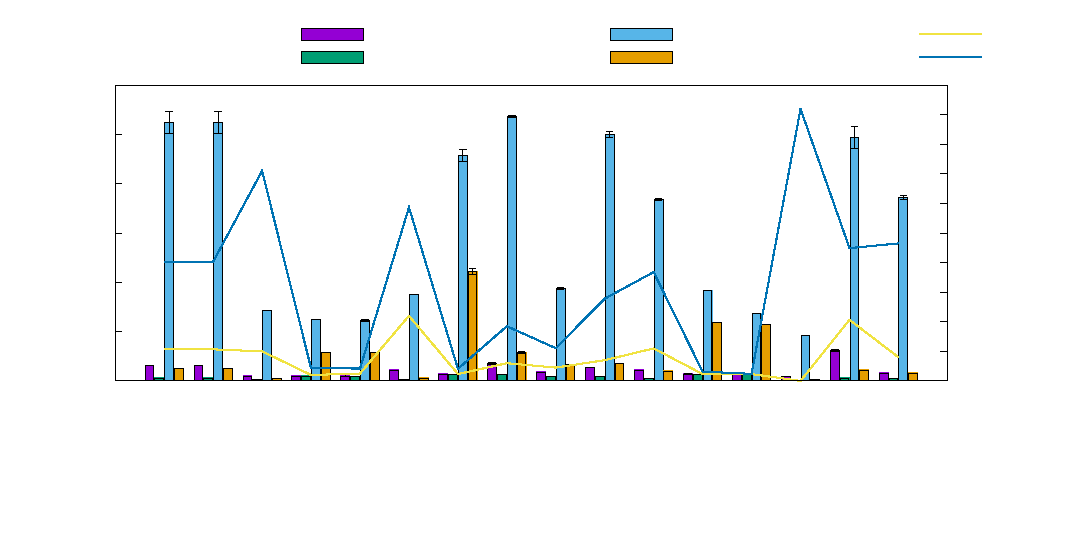
\includegraphics[width={504.00bp},height={252.00bp}]{all-hist-SetupTimesec}}%
    \gplfronttext
  \end{picture}%
\endgroup

\caption{Setup Time of Benchmarks}
\label{fig:graph_setup_time}
\end{figure*}

\subsection{Discussion}
\ana{Ana todo: Discuss why we are slower than HyCC --- because of ad-hoc div-and-conquer optimizations. Have to summarize what Ben and I figured out yesterday.}

\ana{If we can add that our cost model works great (it does!), that would be great but probably won't have time...}


% Related Work Section
\section{Related Work}
\label{sec:related}

\paragraph{MPC languages and compilers.}

Languages and compilers for secure computation have seen significant attention and advances in recent years. The early MPC compilers Fairplay~\cite{CCS:BenNisPin08},
and Sharemind~\cite{ESORICS:BogLauWil08} were followed by PICCO~\cite{CCS:ZhaSteBla13}, Obliv-C~\cite{Zahur:2015}, TinyGarble~\cite{SP:SHSSK15},
Wystiria~\cite{SP:RasHamHic14}, and others. A new generation of MPC compilers
includes SPDZ/SCALE-MAMBA/MP-SPDZ~\cite{Keller:2020} and the ABY/HyCC/MOTION~\cite{NDSS:DemSchZoh15,CCS:BDKKS18,Braun:2022} frameworks.
These two families are the state-of-the art and
are actively developed. Another recent development is Viaduct, a functional language and compiler that supports a range of secure computation
frameworks, including MPC and ZKP. Hastings et el. present a review of compiler frameworks~\cite{Hastings:2019}.

While each of these languages and compilers brings in new ideas and advances, none addresses the problem of ``circuit independent'' intermediate
representation and optimization. We envision a classical compiler structure: (1) a Wysteria, Viaduct, Obliv-C, or IMP Source front end, including rich type systems and
AST-level semantic analysis, compile into the MPC Source IR, (2) MPC Source-level optimizations take place, followed by (3) back-end compilers into circuits.
Our focus is at the intermediate level.

%{\begin{center}
%\includegraphics[width=0.5\linewidth]{figs/focus.png}
%\end{center}
%}

Many works focus on the implementation of MPC protocols exposing an API to the programmer. For example, the ABY/MOTION line of
compiler frameworks provides a library of MPC primitives; the programmer writes MPC programs in C++ on top of the library. These back ends implement
different protocols and allow for mixing, but notably, they leave it to the programer to assign different protocols to different parts of the
computation and perform share conversion accordingly. In addition, MOTION provides SIMD primitives, which allows for efficient execution
of MPC operations, but again, using SIMD primitives is the responsibility of the programer. There is interest in frameworks for automatic mixing,
e.g., \cite{CCS:BDKKS18,Ishaq:2019,Fang:2022}.

Other works, e.g., Obliv-C~\cite{Zahur:2015}, Wystiria~\cite{SP:RasHamHic14} and Viaduct~\cite{Acay:2021} focus on higher-level language design, particularly information-flow systems that
restrict flow between secure and insecure parts of the program.

\ana{Add discussion on HyCC/Buscher here. 1. Formalization, reasoning about correctness of transformation.}
%Key ideas such as ${\sf insecure} <: {\sf secure}$ qualifier systems are similar to the ideas we
%present in~\Secref{sec:interprocedural} and~\Secref{sec:zkp} and we intend to draw on these work. While we will design a high-level language expanding our
%intraprocedural IMP-MPC syntax and semantics into the \emph{interprocedural} case, our interest and focus lie primarily in the ``machine-independent'' optimizations
%thrust of the proposal.

%There is significant development in ZKP languages as well. ~\ana{Alex Ozdemir's talk, ZoKrates, Cairo, others} Our work focuses on ZKP via MPC and our key idea
%is the separation of the higher-level ``backend-independent'' compilation and optimization and the lower-level compilation into circuits.

\paragraph{Classical HPC compilers.}
Automatic vectorization is a longstanding problem in high-performance computing (HPC).
There are thousands of works in this area reflecting over 40 years of research. We presented a vectorization
algorithm for MPC Source, essentially extending classical loop vectorization \cite{Allen:1987}. In HPC vectorization, conditional control flow
presents a challenge --- one cannot estimate the cost of a schedule or vectorize branches in a straightforward manner --- in contrast to
MPC Source vectorization.
We view Karrenberg's work on Whole function vectorization~\cite{Karrenberg:2015} as most closely related to ours --- it linearizes the program and vectorizes
both branches of a conditional applying masking to avoid execution of the branch-not-taken code, and selection (similar to MUX) to select the correct value based on the
result of the condition at runtime.
The problem is that masking and selection, or more generally, handling control predicates~\cite{Benabderrahmane:2010,Karrenberg:2015},
can lead to \emph{slowdown}.
%As a result, vectorizing compilers and polyhedral compilers tend to focus on straight-line code due to the unpredictable
%overhead conditionals may introduce. \ana{add Louis noel pochet's benchmarks. citation on vectorizing compilers???}

We argue that vectorization over linear MPC Source is a different problem, one that warrants a new look, while drawing from
results in HPC.
Since both branches of the conditional and the multiplexer \emph{always} execute, not only can we apply aggressive vectorization on linear code, but (perhaps more importantly)
we can also build analytical models that accurately predict execution time. These models in turn would drive optimizations such as vectorization, protocol mixing, and others.
Vectorization meshes in with those additional optimizations in non-trivial ways.

Furthermore, extensions of classical loop vectorization with array writes, arbitrary indexing, including non-affine indexing, and interaction with SSA are non-trivial
and present novel challenges and opportunities for contribution. Polyhedral parallelization~\cite{Benabderrahmane:2010} considers a higher-level source (typically AST)
representation, while our work takes advantage of linear MPC Source and SSA form. The work by Karrenberg~\cite{Karrenberg:2015} is rare in that space, in the sense that it considers
vectorization over SSA form, which has similarities to MPC Source. We consider different array representation, notion of dependence, and reasoning
about dependence, which we conjecture is more suitable for MPC Source. Buscher~\cite{Buscher:2018} considers SIMD-vectorization
at the level of source code, which then combines with circuit-level optimizations in the TinyGarble compiler.
He proposes using an off-the-shelf polyhedral compiler, however, application is limited to only two routines,
essentially just inner product and euclidian distance; it is unclear how effective the off-the-shelf compiler is.
In contrast, we consider vectorization at the level of MPC Source separating ``backend-independent'' vectorization
and circuit-level amortization (done by MOTION). We apply our compiler on a wide range of routines.


%\section{Future Work}
%\label{sec:implementation_and_benchmarks}
%\input{../sections/implementation_and_benchmarks.tex}
%\input{../sections/evaluation.tex}

\section{Conclusion and Future Work}
\label{sec:conclusion}

\ana{Need a conclusion here!}

%\input{../sections/conclusion.tex}

%\begin{acks}
%    \ishaq{TODO}
%\end{acks}

%\printbibliography

\bibliographystyle{plain}
%\bibliography{c:/trink/Doc/MyTexFiles/texrefs}
%\bibliography{mybib,library,library1,library2,library3,library_ana}
\bibliography{library_ana,crypto_crossref}


% that's all folks
\end{document}


